%%%%%%%%%%%%%%%%%%%%%%%%%%%%%%%%%%%%%%%%%%%%%%
%
%		Thesis Settings
%
%		EDOC Template
%		2011
%
%%%%%%%%%%%%%%%%%%%%%%%%%%%%%%%%%%%%%%%%%%%%%%
\documentclass[a4paper,11pt,fleqn]{book}

\usepackage[T1]{fontenc}
\usepackage[utf8]{inputenc}
\usepackage[french,german,english]{babel}

%%%%%%%%%%%%%%%%%%%%%%%%%%%%%%%%%%%%%%%%%%%%%%%
%% EDOC THESIS TEMPLATE: Variant 1.0 -> Latin modern, large text width&height
%%%%%%%%%%%%%%%%%%%%%%%%%%%%%%%%%%%%%%%%%%%%%%%
%\usepackage{lmodern}
%\usepackage[a4paper,top=22mm,bottom=28mm,inner=35mm,outer=25mm]{geometry}
%%%%%%%%%%%%%%%%%%%%%%%%%%%%%%%%%%%%%%%%%%%%%%%

%%%%%%%%%%%%%%%%%%%%%%%%%%%%%%%%%%%%%%%%%%%%%%
% EDOC THESIS TEMPLATE: Variant 2.0 -> Utopia, Gabarrit A (lighter pages)
%%%%%%%%%%%%%%%%%%%%%%%%%%%%%%%%%%%%%%%%%%%%%%
\usepackage{fourier} % Utopia font-typesetting including mathematical formula compatible with newer TeX-Distributions (>2010)
%\usepackage{utopia} % on older systems -> use this package instead of fourier in combination with mathdesign for better looking results
%\usepackage[adobe-utopia]{mathdesign}
\setlength{\textwidth}{146.8mm} % = 210mm - 37mm - 26.2mm
\setlength{\oddsidemargin}{11.6mm} % 37mm - 1in (from hoffset)
\setlength{\evensidemargin}{0.8mm} % = 26.2mm - 1in (from hoffset)
\setlength{\topmargin}{-2.2mm} % = 0mm -1in + 23.2mm 
\setlength{\textheight}{221.9mm} % = 297mm -29.5mm -31.6mm - 14mm (12 to accomodate footline with pagenumber)
\setlength{\headheight}{14pt}
%%%%%%%%%%%%%%%%%%%%%%%%%%%%%%%%%%%%%%%%%%%%%%



\setlength{\parindent}{0pt}

\usepackage{setspace} % increase interline spacing slightly
\setstretch{1.1}

\makeatletter
\setlength{\@fptop}{0pt}  % for aligning all floating figures/tables etc... to the top margin
\makeatother


\usepackage{graphicx,xcolor}
\graphicspath{{images/}}

\usepackage{subfig}
\usepackage{booktabs}
\usepackage{lipsum}
\usepackage{microtype}
\usepackage{url}
\usepackage[final]{pdfpages}

\usepackage{fancyhdr}
\renewcommand{\sectionmark}[1]{\markright{\thesection\ #1}}
\pagestyle{fancy}
	\fancyhf{}
	\renewcommand{\headrulewidth}{0.4pt}
	\renewcommand{\footrulewidth}{0pt}
	\fancyhead[OR]{\bfseries \nouppercase{\rightmark}}
	\fancyhead[EL]{\bfseries \nouppercase{\leftmark}}
	\fancyfoot[EL,OR]{\thepage}
\fancypagestyle{plain}{
	\fancyhf{}
	\renewcommand{\headrulewidth}{0pt}
	\renewcommand{\footrulewidth}{0pt}
	\fancyfoot[EL,OR]{\thepage}}
\fancypagestyle{addpagenumbersforpdfimports}{
	\fancyhead{}
	\renewcommand{\headrulewidth}{0pt}
	\fancyfoot{}
	\fancyfoot[RO,LE]{\thepage}
}

\usepackage{listings}
\lstset{language=[LaTeX]Tex,tabsize=4, basicstyle=\scriptsize\ttfamily, showstringspaces=false, numbers=left, numberstyle=\tiny, numbersep=10pt, breaklines=true, breakautoindent=true, breakindent=10pt}

\usepackage{hyperref}
\hypersetup{pdfborder={0 0 0},
	colorlinks=true,
	linkcolor=black,
	citecolor=black,
	urlcolor=black}
\urlstyle{same}

\makeatletter
\def\cleardoublepage{\clearpage\if@twoside \ifodd\c@page\else
    \hbox{}
    \thispagestyle{empty}
    \newpage
    \if@twocolumn\hbox{}\newpage\fi\fi\fi}
\makeatother \clearpage{\pagestyle{plain}\cleardoublepage}


%%%%% CHAPTER HEADER %%%%
\usepackage{color}
\usepackage{tikz}
\usepackage[explicit]{titlesec}
\definecolor{ashgrey}{rgb}{0.7, 0.75, 0.71}
\newcommand*\chapterlabel{}
%\renewcommand{\thechapter}{\Roman{chapter}}
\titleformat{\chapter}[display]  % type (section,chapter,etc...) to vary,  shape (eg display-type)
	{\normalfont\bfseries\Huge} % format of the chapter
	{\gdef\chapterlabel{\thechapter\ }}     % the label 
 	{0pt} % separation between label and chapter-title
 	  {\begin{tikzpicture}[remember picture,overlay]
    \node[yshift=-8cm] at (current page.north west)
      {\begin{tikzpicture}[remember picture, overlay]
        \filldraw[fill=ashgrey, draw=white] (0,0) rectangle(35.5mm,15mm);
        \node[anchor=north east,yshift=-7.2cm,xshift=34mm,minimum height=30mm,inner sep=0mm] at (current page.north west)
        {\parbox[top][30mm][t]{15mm}{\raggedleft $\phantom{\textrm{l}}$\color{white}\chapterlabel}};  %the black l is just to get better base-line alingement
        \node[anchor=north west,yshift=-7.2cm,xshift=37mm,text width=\textwidth,minimum height=30mm,inner sep=0mm] at (current page.north west)
              {\parbox[top][30mm][t]{\textwidth}{\color{black}#1}};
       \end{tikzpicture}
      };
   \end{tikzpicture}
   \gdef\chapterlabel{}
  } % code before the title body

\titlespacing*{\chapter}{0pt}{50pt}{30pt}
\titlespacing*{\section}{0pt}{13.2pt}{*0}  % 13.2pt is line spacing for a text with 11pt font size
\titlespacing*{\subsection}{0pt}{13.2pt}{*0}
\titlespacing*{\subsubsection}{0pt}{13.2pt}{*0}

\newcounter{myparts}
\newcommand*\partlabel{}
\titleformat{\part}[display]  % type (section,chapter,etc...) to vary,  shape (eg display-type)
	{\normalfont\bfseries\Huge} % format of the part
	{\gdef\partlabel{\thepart\ }}     % the label 
 	{0pt} % separation between label and part-title
 	  {\setlength{\unitlength}{20mm}
	  \addtocounter{myparts}{1}
	  \begin{tikzpicture}[remember picture,overlay]
    \node[anchor=north west,xshift=-65mm,yshift=-6.9cm-\value{myparts}*20mm] at (current page.north east) % for unknown reasons: 3mm missing -> 65 instead of 62
      {\begin{tikzpicture}[remember picture, overlay]
        \draw[fill=black] (0,0) rectangle(62mm,20mm);   % -\value{myparts}\unitlength
        \node[anchor=north west,yshift=-6.1cm-\value{myparts}*20mm,xshift=-60.5mm,minimum height=30mm,inner sep=0mm] at (current page.north east)
        {\parbox[top][30mm][t]{55mm}{\raggedright \color{white}Part \partlabel $\phantom{\textrm{l}}$}};  %the phantom l is just to get better base-line alingement
        \node[anchor=north east,yshift=-6.1cm-\value{myparts}*20mm,xshift=-63.5mm,text width=\textwidth,minimum height=30mm,inner sep=0mm] at (current page.north east)
              {\parbox[top][30mm][t]{\textwidth}{\raggedleft \color{black}#1}};
       \end{tikzpicture}
      };
   \end{tikzpicture}
   \gdef\partlabel{}
  } % code before the title body


%\documentclass{egpubl}
%\usepackage{egsgp15}
%\usepackage{t1enc,dfadobe}
%\usepackage{egweblnk}
\usepackage{cite}
\usepackage{amsmath}
\usepackage{microtype}
\usepackage{overpic}
\usepackage{color}
\usepackage{amssymb}
\usepackage{graphicx}
\usepackage{changepage}
\usepackage{hyperref}
\hypersetup{
    colorlinks=true,
    filecolor=magenta,      
    urlcolor=cyan,
}

%%%%%%%%%%%%%%%%%%%%%%%%%%%%%%%%%%%%%%%%%%%%%%
%
%		Thesis Settings
%		Custom settings
%
%		2011
%
%%%%%%%%%%%%%%%%%%%%%%%%%%%%%%%%%%%%%%%%%%%%%%

%
%   Use this file for your own custom packages, command-definitions, etc...
%


% the following lines are for creating a simplified TO-DO box. However since boites is not per default installed with all latex-distributions, we have removed this example again
% if you want to use it and do not have "boites" installed, you can get it from here: http://www.ctan.org/tex-archive/macros/latex/contrib/boites
%
%\usepackage{boites,boites_exemples}
%\newcommand{\todolist}[1]{\begin{boiteepaisseavecuntitre}{TO DO in this chapter} #1 \end{boiteepaisseavecuntitre}}  % creates a little box
% %\newcommand{\todolist}[1]{}  % to be used when to do is not to be printed
  
% Comments
\definecolor{turquoise}{cmyk}{0.65,0,0.1,0.3}
\definecolor{purple}{rgb}{0.65,0,0.65}
\definecolor{dark_green}{rgb}{0, 0.5, 0}
\definecolor{orange}{rgb}{0.8, 0.6, 0.2}
\definecolor{red}{rgb}{0.8, 0.2, 0.2}
\definecolor{blueish}{rgb}{0.0, 0.7, 1}
\definecolor{light_gray}{rgb}{0.7, 0.7, .7}
\definecolor{pink}{rgb}{1, 0, 1}
\newcommand{\edit}[1]{\textcolor{dark_green}{#1}}
\newcommand{\new}[1]{{#1}}
%\newcommand{\LEGACY}[1]{\textcolor{orange}{[LEGACY] #1}}
\newcommand{\aedit}[1]{\textcolor{purple}{#1}}
\newcommand{\ADDRESSED}[1]{{}}
\newcommand{\copypaste}[1]{{#1}}
\newcommand{\revision}[1]{{#1}}
%\newcommand{\hidden}[1]{{}}

%%
%% inlined comments
%% 
\newcommand{\MP}[1]{{\color{orange}[MP: #1]}} % mark 
\newcommand{\AT}[1]{{\color{blueish}[AT: #1]}} % andrea
\newcommand{\SB}[1]{{\color{turquoise}[SB: #1]}} % sofien
\newcommand{\NT}[1]{{\color{dark_green}[NT: #1]}} % anastasia
\newcommand{\MB}[1]{{\color{pink}[MB: #1]}} % mario
\newcommand{\MS}[1]{{\color{purple}[MS: #1]}} % matthias

\newcommand{\yoff}{0}

%%
%% shortcut for references
%% 
\newcommand{\Fig}[1]{Figure~\ref{fig:#1}}
\newcommand{\Figure}[1]{Figure~\ref{fig:#1}}
\newcommand{\Eq}[1]{Equation~\ref{eq:#1}}
\newcommand{\Equation}[1]{Equation~\ref{eq:#1}}
\newcommand{\Sec}[1]{Section~\ref{sec:#1}}
\newcommand{\Section}[1]{Section~\ref{sec:#1}}
\newcommand{\Appendix}[1]{Appendix~\ref{app:#1}}


%%
%% Inlined annotation of paragraph content
%% 
\newcommand{\brief}[1]{} % ONLY LATEX VISIBLE
% \newcommand{\brief}[1]{{\flushright\small{\vspace{-7pt}\color{light_gray} [\textbf{#1}]}\\}}


%%
%% MATH STUFF
%% 
\let\vec=\mathbf
\let\mat=\vec
\newcommand{\F}{F} % dataframe
\newcommand{\normal}{\mathcal{N}}
\newcommand{\vertex}{\mathbf{v}}

% MARIO
\newcommand{\abs}[1]{\left| #1 \right|}
\newcommand{\norm}[1]{\left\Vert {#1} \right\Vert}

% hack to use computer modern font for bold greek letters
\SetSymbolFont{letters}{bold}{OML}{cmm}{b}{it}
\SetSymbolFont{operators}{bold}{OT1}{cmr}{bx}{n}

%%
%% Small math symbols
%%
\newcommand{\unaryminus}{\scalebox{0.5}[1.0]{\( - \)}} % small "-"
% \newcommand{\smallless}{\scalebox{0.5}[.5]{\(<\)}} % small "<"

%--- OLD SYMBOLS
% \newcommand{\pars}{\boldsymbol{\omega}}
% \newcommand{\parsopt}{\boldsymbol{\omega}^*}

%%
%% Inverted
%%
\usepackage[T3,T1]{fontenc}
\DeclareSymbolFont{tipa}{T3}{cmr}{m}{n}
\DeclareMathAccent{\invbreve}{\mathalpha}{tipa}{16}

%%
%% Math symbols
%%
\newcommand{\cyl}{\mathbf{c}} %cylinder
\newcommand{\cylrad}{\mathbf{c}} %cylinder

% weights of terms
\newcommand{\omegacloud}{\omega_1}
\newcommand{\omegasilhouette}{\omega_2}
\newcommand{\omegawrist}{\omega_3}
\newcommand{\omegapcaproj}{\omega_4}
\newcommand{\omegapcareg}{\omega_5}
\newcommand{\omegacollision}{\omega_6}
\newcommand{\omegabounds}{\omega_7}
\newcommand{\omegatemporalst}{\omega_8}
\newcommand{\omegatemporalnd}{\omega_9}
%\newcommand{\skeleton}{\mathcal{K}}
\newcommand{\numpars}{26}
\newcommand{\jacobian}{\mathbf{J}}
\newcommand{\J}{\jacobian}
\newcommand{\Jproj}{\jacobian_{\text{persp}}}
\newcommand{\Jskel}{\jacobian_{\text{skel}}}
\newcommand{\residuals}{\mathbf{e}}
\newcommand{\weight}{\omega}

\newcommand{\pixelHtrack}{\mathbf{p}}
\newcommand{\pixels}{\mathbf{P}}

\newcommand{\pointHtrack}{\mathbf{x}}
\newcommand{\skelpoint}{\mathbf{k}}
\newcommand{\points}{\mathbf{X}}
\newcommand{\proj}{\Pi}
\newcommand{\PointsRender}{\mathcal{X}_{r}}

\newcommand{\PointsSensorHtrack}{\mathcal{X}_{s}}
\newcommand{\DepthRender}{\mathcal{D}_{r}}
\newcommand{\DepthSensor}{\mathcal{D}_{s}} 
\newcommand{\SilhoRender}{\mathcal{S}_{r}}
\newcommand{\SilhoSensor}{\mathcal{S}_{s}}
\newcommand{\DataSensor}{\mathcal{F}}
\newcommand{\history}{\mathcal{H}}
\newcommand{\handmodel}{\mathcal{M}}
\newcommand{\visiblehand}{\invbreve\handmodel}
\newcommand{\posespace}{\mathcal{P}}
\newcommand{\MU}{\boldsymbol\mu} 
\newcommand{\SIGMA}{\boldsymbol{\Sigma}}

\newcommand{\parsHtrack}{\boldsymbol{\theta}}

\newcommand{\dpars}{\Delta\boldsymbol{\theta}}
\newcommand{\parssub}{\tilde{\boldsymbol{\theta}}}
\newcommand{\parsopt}{\pars^*}
\newcommand{\identity}{\mathbf{I}}
\newcommand{\zero}{\mathbf{0}}

% \underset{x}{\operatorname{argmin}} 
\DeclareMathOperator*{\argmin}{arg\,min}
\DeclareMathOperator*{\argmax}{arg\,max}


%--- 2x2 matrix block
\newcommand{\matblocktwo}[4]{
\left[
    \begin{array}{c|c}
        #1 & #2 \\ \hline
        #3 & #4 
    \end{array}
\right] 
}

%--- TO SHOW PATH OF INSERTED IMAGES
\usepackage{currfile}
% \newcommand{\putfilename}{\put(-3,0){\rotatebox{90}{\color{red}\currfilename}}}
\newcommand{\putfilename}{}


\usepackage{overpic}
\usepackage{amssymb}
\usepackage{graphicx}
\usepackage{epstopdf}
\usepackage{amsmath}
\usepackage{graphicx}
\usepackage{amsfonts}
\usepackage{enumitem}
\usepackage{multirow}
\usepackage{algpseudocode}
\usepackage{algorithm,algorithmicx}
\usepackage{xcolor}

%% 
%% Better text layout (ONLY ENABLE IN FINAL!!)
%%
\usepackage{microtype}

% \usepackage{cite}


%% 
%% Insert symbols on figures
%%
\usepackage{overpic}
\usepackage{currfile} % \currfiledir
\usepackage{wrapfig}
\usepackage{graphicx}
\usepackage{caption} % \caption*

%% 
%% More compact paragraphs
%%
% \usepackage{stringstrings} %< TitleCase
\renewcommand{\paragraph}[1]{\textbf{#1.}}

%% 
%% Bibliography
%% 
% \usepackage[backend=biber,sorting=ydnt,style=alphabetic,citestyle=alphabetic,maxbibnames=99]{biblatex}

%%
%% Rotated text
%%
\usepackage{rotating}
\newcommand{\rotninety}[1]{\begin{turn}{90} #1 \end{turn}}

%%
%% text layout
%%
% Insert whitespace at the end of a paragraph
\setlength{\parskip}{.5\baselineskip}%
% Don't intent by default on new paragraph
\setlength{\parindent}{0pt}%

%%
%% PDF comments
%%
\usepackage{pdfcomment}
\providecommand{\AnastasiaComment}[1]{\pdfcomment[color=red,icon=Note]{#1}}

%%
%% margin comments
%%
% \usepackage[colorinlistoftodos]{todonotes}

%% 
%% To define colors
%% 
\usepackage{color}
\definecolor{lightgray}{rgb}{0.64, 0.64, 0.64}
\definecolor{mygray}{gray}{0.6}
\definecolor{darkgreen}{rgb}{0.2, 0.35, 0.385}
\definecolor{lightgreen}{rgb}{0.2, 0.85, 0.385}
 
%% 
%% Portions that {need major work, comments}
%% 
\newenvironment{draft}{\color{red}}{\color{black}}
\newcommand{\INSTRUCTIONS}[1]{{\textcolor{blue}{[INSTRUCTIONS] #1}}}
\newcommand{\OK}{{\textcolor{green}{OK!}}}
\newcommand{\todo}[1]{{\textcolor{red}{#1}}}
\renewcommand{\todo}[1]{{#1}} % DISABLES TODO
\newcommand{\accepted}[1]{{\textcolor{green}{#1}}}
\newcommand{\TODO}[1]{{\textcolor{red}{[TODO: #1]}}}
\newcommand{\ignore}[1]{}
\newenvironment{DRAFT}{\color{red}}{\ignorespacesafterend}
\newcommand{\ATFINISH}{\todo{{----------- ANDREA - FINISHED EDITING HERE -----------}}}


%% 
%% Inlined comments
%% 
\newcommand{\Anastasia}[1]{{\textcolor{PineGreen}{[ANA: #1]}}}


%--- HModel
\newcommand{\FPS}{{\small FPS}}
\newcommand{\skeletonHmodel}{\mathcal{S}}
\newcommand{\surface}{\mathcal{M}}
\newcommand{\model}{\surface}
\newcommand{\implicit}{\phi}
\newcommand{\numblocks}{\todo{20}}
\newcommand{\ball}{\mathcal{B}} %<< ball
\newcommand{\ballcenter}{\mathbf{c}} %<< ball center
\newcommand{\segment}{\overline{\ballcenter_1 \ballcenter_2}} % Segment
\newcommand{\termscalib}{{\mathcal{T}_\text{calib}}}
\newcommand{\termstrack}{{\mathcal{T}_\text{track}}}
\newcommand{\skewproj}{\mathbf{s}} % Skewed projection
\newcommand{\depth}{\mathcal{D}}
\newcommand{\parsHmodel}{\boldsymbol{\Theta}}
\newcommand{\parpose}{\boldsymbol{\theta}}
\newcommand{\parposes}{{\{\boldsymbol{\theta}_n\}}}
\newcommand{\parposture}{\bar{\boldsymbol{\delta}}}
\newcommand{\centers}{{\mathbf{C}}}
\newcommand{\restcenters}{{\mathbf{\bar{C}}}}
\newcommand{\posedcenters}{{\{\mathbf{C}_n\}}}
\newcommand{\radii}{{\mathbf{\bar{r}}}}
\newcommand{\chain}{\mathcal{K}}
\newcommand{\edge}{\mathbf{e}}
\newcommand{\dataset}[1]{\todo{dataset/#1}}
\newcommand{\realsense}{\emph{Intel RealSense}}
\newcommand{\kinectone}{\emph{Microsoft KinectOne}}
\providecommand{\depthrend}{\mathcal{R}}
\providecommand{\metricone}{E_\text{3D}}
\providecommand{\metrictwo}{E_\text{2D}}
\newcommand{\dexter}{\emph{\textsc{Dexter}}}
\newcommand{\fingerpaint}{\emph{\textsc{FingerPaint}}}
\newcommand{\handy}{\emph{\textsc{handy}}}
\newcommand{\handyseq}[1]{\emph{\textsc{handy/#1}}}
\newcommand{\metric}{\varphi}

%--- HTrack
\newcommand{\PointsSensorHmodel}{\mathcal{P}_{s}}
\newcommand{\pointHmodel}{\mathbf{p}}
\newcommand{\pixelHmodel}{\mathbf{x}}
\newcommand{\footpoint}{\mathbf{q}}
\newcommand{\element}{\mathcal{E}^e}
\newcommand{\oneelement}{\mathcal{E}}
\newcommand{\camdir}{\mathbf{v}}
\newcommand{\citeme}{[Proposed Method]}

% \newcommand{\Video}[1]{Video~\todo{[#1]}}
%--- Specific video entries
\newcommand{\VideoTeaser}{{Video~{[02:57]}}}
\newcommand{\VideoHTrack}{{Video~{[03:53]}}}
\newcommand{\VideoElements}{{Video~{[00:58]}}}
\newcommand{\VideoKinematic}{{Video~{[02:12]}}}
\newcommand{\VideoMVS}{{Video~{[01:30]}}}
\newcommand{\VideoCalibRGB}{{Video~{[01:45]}}}
\newcommand{\VideoSpace}{{Video~{[02:51]}}}
\newcommand{\VideoNoJointCollapse}{{Video~{[01:18]}}}

% \newcommand{\VideoExtra}[1]{Video~2~\todo{[#1]}}

\newcommand{\VideoExtra}{{Video~{[04:50]}}} % start
\newcommand{\VideoExtraTaylOne}{{Video~{[04:53]}}}
\newcommand{\VideoExtraSridOne}{{Video~{[05:40]}}}
\newcommand{\VideoExtraSridTwo}{{Video~{[05:56]}}}
\newcommand{\VideoExtraSridThree}{{Video~{[06:15]}}}
\newcommand{\VideoExtraSridFour}{{Video~{[06:29]}}}
\newcommand{\VideoExtraSharOne}{{Video~{[07:33]}}}
\newcommand{\VideoExtraSharTwo}{{Video~{[08:07]}}}
\newcommand{\VideoExtraSharThree}{{Video~{[08:37]}}}

%--- Video limitations
\newcommand{\VideoLimitationsHmodel}{{Video~{{[09:56]}}}}
\newcommand{\VideoLimFramerate}{{Video~{{[11:02]}}}}
\newcommand{\VideoLimOcclusions}{{Video~{{[10:30]}}}}

\usepackage{overpic}
\usepackage{amssymb}
\usepackage{graphicx}
\usepackage{mathrsfs}
\usepackage{xcolor}
\usepackage{float} %< to define algorithms
\usepackage{anyfontsize} %< remove warnings
\usepackage{sidecap} %< caption on side

%%
%% general comments
%% 
% \usepackage{color}
\definecolor{turquoise}{cmyk}{0.65,0,0.1,0.3}
\definecolor{purple}{rgb}{0.65,0,0.65}
\definecolor{dark_green}{rgb}{0, 0.5, 0}
\definecolor{orange}{rgb}{0.8, 0.6, 0.2}
\definecolor{red}{rgb}{0.8, 0.2, 0.2}
\definecolor{blueish}{rgb}{0.0, 0.7, 1}
\definecolor{light_gray}{rgb}{0.7, 0.7, .7}
\definecolor{pink}{rgb}{1, 0, 1}
\definecolor{accent}{rgb}{179,81,109}
\definecolor{anagreen}{rgb}{.13,.627,.494}
\definecolor{anasalmon}{rgb}{.85,.604,.564}

%%
%% general comments
%% 
\newcommand{\hidden}[1]{{}} %< discards
\newcommand{\LEGACY}[1]{\textcolor{orange}{[LEGACY] #1}}
\newcommand{\todo}[1]{{\color{red}#1}}
\newcommand{\red}[1]{{\color{red}#1}}
\newcommand{\TODO}[1]{{\color{red}[TODO: #1]}}
\newcommand{\ADDRESSED}[1]{{}}
\newcommand{\copypaste}[1]{{#1}}
\newcommand{\revision}[1]{{#1}}
%\newcommand{\revision}[1]{{\color{red}#1}}
\newenvironment{DRAFT}{\colorlet{oldcolor}{.} \color{red}}{\color{oldcolor}}
% \newenvironment{edit}{\colorlet{oldcolor}{.} \color{dark_green}}{\color{oldcolor}}
\newenvironment{edit}{\colorlet{oldcolor}{.}}{\color{oldcolor}}

%%
%% personal comments
%% 
\newcommand{\AN}[1]{{\color{teal}[AN: #1]}} % anastasia 
\newcommand{\AT}[1]{{\color{pink}[AT: #1]}} % andrea
\newcommand{\MP}[1]{{\color{blueish}[MP: #1]}} % mark
\newcommand{\ER}[1]{{\color{orange}[ER: #1]}} % edo
\newcommand{\AF}[1]{{\color{blueish}[AF: #1]}} % andrew

%%
%% shortcut for references
%% 
\newcommand{\Fig}[1]{Fig.~\ref{fig:#1}}
\newcommand{\Figure}[1]{Figure~\ref{fig:#1}}
\newcommand{\Eq}[1]{Eq.~\ref{eq:#1}}
\newcommand{\Equation}[1]{Equation~\ref{eq:#1}}
\newcommand{\Optimization}[1]{Optimization~\ref{eq:#1}}
\newcommand{\Sec}[1]{Sec.~\ref{sec:#1}}
\newcommand{\Section}[1]{Section~\ref{sec:#1}}
\newcommand{\Appendix}[1]{Appendix~\ref{app:#1}}

%%
%% Inlined annotation of paragraph content
%% 
\newcommand{\brief}[1]{} % ONLY LATEX VISIBLE
% \newcommand{\brief}[1]{{\flushright\small{\vspace{-7pt}\color{light_gray} [\textbf{#1}]}\\}}

%%
%% SHOW PATH OF INSERTED IMAGES
%% 
\usepackage{currfile}
\newcommand{\putfilename}{}
% \newcommand{\putfilename}{ \put(-3,0){\rotatebox{90}{\color{red}\currfilename}}}

% Vertical text
\newcommand{\vertical}[1]{\rotatebox{90}{#1}}

%%
%% text layout
%%
% Insert whitespace at the end of a paragraph
\setlength{\parskip}{.5\baselineskip}%
% Don't intent by default on new paragraph
\setlength{\parindent}{0pt}%


%%
%% text layout
%%
\renewcommand{\paragraph}[1]{{\textbf{#1.}}}

%%
%% figure labels
%%
% \newcommand{\myfigurename}{\put(-4,0){\vertical{\todo{\currfiledir}}}}
\newcommand{\myfigurename}{}

%%
%% algorithm float (instead of table)
%%
\floatstyle{boxed}
\newfloat{algorithm}{t}{alg}
\floatname{algorithm}{Table}
\newcommand{\Tab}[1]{Tab.~\ref{tab:#1}}
\newcommand{\Table}[1]{Table~\ref{tab:#1}}
%%
%% MATH STUFF
%% 
\newcommand{\bs}{\boldsymbol}
\let\vec=\mathbf
\let\mat=\vec

\newcommand{\hessian}{H}
\newcommand{\shape}{\beta}
\newcommand{\cov}{\Sigma}
\newcommand{\gaussian}[2]{\mathcal{N}(#1,#2)}
\renewcommand{\star}[1]{{#1}^*}

%--- Video Timings
\newcommand{\Video}[1]{Video~[#1]}
\newcommand{\VideoSynth}{\Video{03:16}}
\newcommand{\VideoReal}{\Video{03:41}}
\newcommand{\VideoQualitative}{\Video{04:03}}
\newcommand{\VideoNYU}{\TODO{\Video{00:00}}}
\newcommand{\VideoHandy}{\TODO{\Video{00:00}}}

%--- Macro for names
\newcommand{\OfflineSoft}{Offline-Soft}
\newcommand{\OfflineHard}{Offline-Hard}

\newcommand{\F}{F} % dataframe
\newcommand{\normal}{\mathcal{N}}
\newcommand{\vertex}{\mathbf{v}}
\newcommand{\abs}[1]{\left| #1 \right|}
\newcommand{\norm}[1]{\left\Vert {#1} \right\Vert}
% hack to use computer modern font for bold greek letters
\SetSymbolFont{letters}{bold}{OML}{cmm}{b}{it}
\SetSymbolFont{operators}{bold}{OT1}{cmr}{bx}{n}
% Small math symbols
\newcommand{\unaryminus}{\scalebox{0.5}[1.0]{\( - \)}} % small "-"
\newcommand{\smallless}{\scalebox{0.5}[.5]{\(<\)}} % small "<"
% \underset{x}{\operatorname{argmin}} 
\DeclareMathOperator*{\argmin}{arg\,min}
\DeclareMathOperator*{\argmax}{arg\,max}
% 2x2 matrix block
\newcommand{\matblocktwo}[4]{ \left[ \begin{array}{c|c} #1 & #2 \\ \hline #3 & #4 \end{array} \right]}





\begin{document}
\frontmatter
\begin{titlepage}
\begin{center}
%\large
\sffamily


\null\vspace{2cm}
{\huge Real-Time Generative \\[12pt] Hand Modeling and Tracking } \\[24pt] 
\textcolor{gray}{\small{THIS IS A TEMPORARY TITLE PAGE \\ It will be replaced for the final print by a version \\ provided by the service academique.}}
    
\vfill

\begin{tabular} {cc}
\parbox{0.3\textwidth}{
\includegraphics[width=4cm]{images/epfl}}
&
\parbox{0.7\textwidth}{%
	%Thèse n. ---- 2018\\
	%présenté le 29 Mars 2018\\
	Thèse présenté le 29 Mars 2018\\
	à la Faculté Informatique et Communications \\
	Laboratoire d’Informatique Graphique et Géométrique \\
	programme doctoral en Informatique et Communications \\
	École Polytechnique Fédérale de Lausanne\\[6pt]
	pour l'obtention du grade de Docteur ès Sciences\\
	par\\ [4pt]
	\null \hspace{3em} Anastasia Tkach\\[9pt]
%
\small
Jury de thèse:\\[4pt]
%acceptée sur proposition du jury:\\[4pt]
%
    Prof. Pascal Fua, président du jury\\
    Prof. Mark Pauly, directeur de thèse\\
    Prof. Andrea Tagliasacchi, co-directeur de thèse\\
    Prof. Vincent Lepetit, rapporteur\\
    Dr. Gerard Pons-Moll, rapporteur\\
    Dr. Mathieu Salzmann, rapporteur\\[12pt]
%
Lausanne, EPFL, 2018}
\end{tabular}
\end{center}
\vspace{2cm}
\end{titlepage}




%\cleardoublepage
\thispagestyle{empty}


\vspace*{3cm}

\begin{raggedleft}
    	Wings are a constraint that makes \\
	it possible to fly.\\
     --- Robert Bringhurst\\
\end{raggedleft}

\vspace{4cm}

\begin{center}
    To my parents\dots
\end{center}



%\chapter*{Acknowledgements}
\markboth{Acknowledgements}{Acknowledgements}
\addcontentsline{toc}{chapter}{Acknowledgements}
% put your text here
First of all, I would like to thank my advisors Mark Pauly and Andrea Tagliasacchi.

I am grateful to Mark for hiring me to work on hand tracking. This topic was in demand at the start of my PhD and it is even more so at the time of my graduation. Thanks to Mark, my first project was extremely well chosen. I was not starting from scratch, but working in a team of experienced researchers. The techniques that I learned fueled my entire PhD. Another crucial point that I want to thank for is freedom that I was given. I came to doctoral school with a goal to become an independent researcher which is impossible without some freedom to choose work directions and make mistakes.

I would like to express my deepest gratitude to Andrea Tagliasacchi. I was inspired by his energy, devotion to research and even more so by his long term vision and revolutionary ideas. Also I am grateful for his patience, and technical and moral support at difficult stages of my research. Andrea guided me through stagnation and dead ends to accepted papers. It motivated me a lot to see that he personally cares about success and well-being of his students and is ready to make big efforts to help. I would like to express my hope that our collaboration will go on for decades.

I am thankful to Sofien Bouaziz for supervising my Master Thesis and co-supervising my first PhD projects. Sofien was always there for me to give technical advice, answer questions or simply cheer me up. I owe Sofien my lucky choice career, since I joined the lab to continue working with him.

I would like to extend my gratitude to my collaborators Mario Botsch, Andrew Fitzgibbon, Edoardo Remelli and Matthias Schröder. The presence of Matthias brightened the deadline for our first project. The company of Edoardo and the possibility to discuss the technical details of the project on the daily basis made the last year my PhD more fun.

I would like to thank Andrew Fitzgibbon for supervising my internship at Microsoft Research. It was a privilege to have weekly discussions and look at the way he approaches research problems. I am also grateful to Federica Bogo and Tom Cashman for their help and advice.

I am thankful to Luciano Sbaiz and Wei Li for mentoring my internship at Google Research. It was an intense learning experience and their guidance and support made a big difference.

I am thankful to my thesis committee for finding the time in their busy schedule to review my thesis and conduct the oral exam: Mario Botsch, Mark Pauly, Mathieu Salzmann, Andrea Tagliasacchi and Jonathan Taylor.

I am grateful to Merlin Nimier-David for his huge help in creating the template hand model. I also thank Timur Bagautdinov, Pierre Baqué, Jan Bednarik, Pei-I Chen, Alexis Dewaele, Fabrice Guibert, Tomas Joveniaux, Isinsu Katircioglu, Mina Konakovic, Andrii Maksai, Hannah Pauly, Edoardo Remelli, Madeleine Robert, Stefano Savare and Matthieu Sauvé for participation in creating online hand calibration dataset.

I would like to thank my LGG lab mates for sharing this experience with me: Sofien Bouaziz, Duygu Ceylan, Minh Dang, Mario Deuss, Alexandru-Eugen Ichim, Mina Konakovic, Stefan Lienhard, Peng Song, Yuliy Schwartzburg, Andrea Tagliasacchi, Ziqi Wang. I am grateful to Madeleine Robert for all the help. In general I thank my fellow PhD students in EDIC for their company, especially the ones who came to board games nights and my collocation neighbors Arseniy Zaostrovnykh and Dmitrii Ustiugov.

Finally, my biggest thanks go to my parents and my life partner Andrii for their love and support. Thank you, Andrii, sharing with me every moment and making me happy.

My research has been supported by the funding from FNS project 200021\_153567.

%\bigskip
 
%\noindent\textit{Lausanne, 12 Mars 2011}
%\hfill D.~K.

%\chapter*{Preface}
\markboth{Preface}{Preface}
\addcontentsline{toc}{chapter}{Preface}
% put your text here
A preface is not mandatory. It would typically be written by some other person (eg your thesis director).

\lipsum[1-2]

\bigskip
 
\noindent\textit{Lausanne, 12 Mars 2011}
\hfill T.~D.

%%\begingroup
%\let\cleardoublepage\clearpage


% English abstract
\cleardoublepage
\chapter*{Abstract}
%\markboth{Abstract}{Abstract}
\addcontentsline{toc}{chapter}{Abstract (English/Français/Deutsch)} % adds an entry to the table of contents
% put your text here
\lipsum[1-2]




% German abstract
\begin{otherlanguage}{german}
\cleardoublepage
\chapter*{Zusammenfassung}
%\markboth{Zusammenfassung}{Zusammenfassung}
% put your text here
\lipsum[1-2]
\end{otherlanguage}




% French abstract
\begin{otherlanguage}{french}
\cleardoublepage
\chapter*{Résumé}
%\markboth{Résumé}{Résumé}
% put your text here
\lipsum[1-2]
\end{otherlanguage}


%\endgroup			
%\vfill


\tableofcontents
%\addcontentsline{toc}{chapter}{List of figures} % adds an entry to the table of contents
%\listoffigures
%\addcontentsline{toc}{chapter}{List of tables} % adds an entry to the table of contents
%\listoftables

\setlength{\parskip}{1em}

\mainmatter


\chapter{Introduction}

\section{Motivation}

\subsection*{Applications}

Tracking and humans in motion is a fundamental problem in computer graphics and computer vision. A particularly important question is how to accurately reconstruct the shape and articulation of human hands. Firstly, because in our everyday life we interact with the surrounding environment using our hands. Secondly, hand motion is a crucial component of non-verbal communication. The digital world applications of hand tracking follow from these two functions of hands in real world.

\paragraph{Performance capture} Performance capture is essential in film and game production for pre-visualization, where motion can be transferred in real-time to a virtual avatar. This allows directors to plan shots more effectively, reduce turn-around times and hence costs. 

\paragraph{Remote communication} Being an important part of our body language, hand motion  plays an important role in the animation of humanoid avatars. The first steps towards commercial avatar-based communication were already made by 
%
\textit{Microsoft Holoportation}
\footnote{\href{https://www.microsoft.com/en-us/research/project/holoportation-3/}{Microsoft Holoportation}, accessed on 27.11.2017}
%
and \textit{Apple Animoji} 
\footnote{\href{https://support.apple.com/en-us/HT208190}{Apple Animoji}, accessed on 27.11.2017}.

\paragraph{Gesture control} Gesture control, a simplified version of hand tracking, becomes increasingly popular as a replacement of remote control for home appliances. It is currently used in such consumer products as 
%
\textit{Samsung Smart TV}
\footnote{\href{http://www.samsung.com/ph/smarttv/motion_control.html}{Samsung Smart TV}, accessed on 27.11.2017}
%
 and \textit{Singlecue}
 \footnote{\href{https://singlecue.com/}{Singlecue}, accessed on 27.11.2017}.
%
 A few other similar products are currently under development.

\paragraph{Virtual interaction} Recently the field of virtual and augmented reality (VR/AR) has made a large step forward. A number of VR/AR headsets was released, including 
\textit{Oculus}, \textit{Vive}, \textit{Samsung Gear VR}, \textit{Microsoft Hololens}, \textit{PlayStation VR}, \textit{Google Daydream}, \textit{Microsoft Mixed Reality Headset}, \textit{Intel Project Alloy} and \textit{Meta 2 AR Headset}. The technology is incomplete without providing the user a way to interact with virtual environment. Most of the listed headsets started with dedicated controller devices. However, there in a notion in the field that hand control is more desirable.
%
\textit{Microsoft Hololens}
\footnote{\href{https://www.microsoft.com/en-us/hololens}{Microsoft Hololens}, accessed on 27.11.2017},
%
\textit{Meta 2 AR Headset}
\footnote{\href{https://www.metavision.com/}{Meta 2 AR Headset}, accessed on 27.11.2017} and
%
\textit{Intel Project Alloy} 
\footnote{\href{https://newsroom.intel.com/press-kits/project-alloy/}{Intel Project Alloy}, accessed on 27.11.2017}
%
are already released in a hand-controlled version and the other main manufactures are also currently developing similar technology.
There are several reasons why VR/AR helmets benefit from hand control. Firstly, according to the user study conducted by 
%
\textit{Leap Motion}
\footnote{\href{http://blog.leapmotion.com/image-hands-bring-your-own-hands-into-virtual-reality/}{Leap Motion Blog}, accessed on 27.11.2017},
%
interacting with your own hands creates a more immersive experience. Secondly, it takes time to get used to the controller device and to remember the functionality assigned to each button. Moreover, hands control can potentially more expressive and subtle than a dedicated controller device.

The commercial hand control devices are still an immerging technology, because hand tracking is challenging and remains a research problem. This was even more so at the start of my doctoral studies. The challenges are described below.

\subsection*{Requirements}

Any consumer application relies on robustness of the tracker. However, the applications listed above have different requirements to the precision, efficiency and output format of hand tracking algorithm.

\textit{Gesture control} system is only required to determine type of gesture, thus even inferring the exact hand pose is not necessary. For \textit{performance capture} it is acceptable have under real time performance. In \textit{remote communication}, if hand motion is re-targeted to an avatar, it only requires tracking joint positions as opposed to hand surface.

\textit{Virtual interaction} is the most demanding, yet most promising application. It requires precise tracking of hand movements. As explained below, precise tracking is only possible if the model is precisely calibration to the user. Moreover, to be suitable for consumer application, it is undesirable for calibration to take long time or require user input. Physically plausible interaction with virtual object requires the system to infer not just hand joint positions, but the volumetric hand model surface.

\subsection*{Challenges}

\paragraph{Tracking challenges} Accurate hand tracking with a non-invasive sensing device in realtime is a challenging scientific problem. Human hands are highly articulated and therefore require models with sufficiently many degrees of freedom to adequately describe the corresponding motion space. Hand motion is often fast and exhibits intricate geometric configurations with complex contact patterns among fingers. With a single-camera RGBD setup, we are faced with incomplete data due to self-occlusions and high noise levels.  

\paragraph{Calibration challenges} Hight precision model based tracking is impossible without calibrating the model to the specific user. The main challenge comes from the fact that tracking and calibration procedures are interdependent. High quality tracking requires good calibration and, to accurately calibrate the model, the motion needs to be precisely tracked. Moreover, hand calibration is bound to consider multiple frames, since from a single frame only a subset of the shape degrees of freedom can be estimated. For example, it is difficult to estimate the length of a phalanx when observing a straight finger.

\subsection*{Setup}

\paragraph{Tracking setup} Over the past two decades a number of techniques have been explored to address hand tacking problem, from expensive and unwieldy marker-based mocap \cite{mocapsurvey} to instrumented gloves \cite{dipietro2008survey} as well as imaging systems \cite{erol2007vision}. Multi-camera imaging systems can recover the hand pose and hand-objects interactions with high accuracy \cite{ballan2013salient}, but the only system capable to approach interactive applications is the 10Hz system of \cite{sridhar2013multicam}. Conversely, in this paper we focus on hand motion tracking with a single RGBD sensor (e.g. Intel RealSense or Microsoft Kinect), commonly predicted to be readily available in a typical AR/VR consumer experience.
We focus on hand motion tracking with a single RGBD sensor (e.g. Intel RealSense or Microsoft Kinect), commonly predicted to be readily available in a typical AR/VR consumer experience. This setup does not require the user to wear a glove or markers. Such single-camera acquisition is particularly advantageous as it is cheap, does not require any sensor calibration, and does not impede user movements.

\paragraph{Tracking: discriminative vs. generative} Modern systems for real-time tracking from RGBD data \cite{sridhar2015fast,sharp2015accurate} rely on a combination of discriminative approaches like \cite{keskin2012hand}, and generative approaches such as \cite{oiko2011hand}. The per-frame re-initialization of discriminative methods prevents error propagation by offering a continuous recovery from tracking failure. As these discriminative models are learnt from data, they are typically limited in their precision by dataset annotation accuracy. Annotating joint locations is challenging because it needs to be done in 3D and because the joints are situated inside of the hand. These difficulties reflect on the labeling quality. Therefore, generative models are used to refine the estimate by aligning a geometric template of the user hand to the measured point cloud as well as to regularize its motion through time. It is not surprising that the quality of the template directly affects the quality of pose refinement.

\paragraph{Calibration setup} The process of accurately generating a user-specific tracking model from input data is referred to in the literature as calibration or personalization. Calibrating a template from a set of static poses is a standard component in the workflow of facial performance capture \cite{weise2011realtime,cao2015facial}, and the work of \cite{taylor2014user} pioneered it within the realm of hand tracking. However, current methods such as \cite{taylor2016joint} suffer a major drawback: the template must be created during a controlled calibration stage, where the hand is scanned in several static poses (i.e. offline). While appropriate for professional use, a calibration session is a severe drawback for seamless deployment in consumer-level applications. 


\section{Contributions}

This dissertation is based on and uses parts of the following papers published in
the course of my PhD:

\begin{adjustwidth}{2.5em}{0pt}
\textsc{Tagliasacchi A., Schroeder M., Tkach A., Bouaziz S., Botsch M., Pauly
M.}: Robust articulated-icp for real-time hand tracking. \textit{Computer Graphics
Forum(Proc. of the Symposium on Geometry Processing) (2015)}.

\textsc{Tkach A., Pauly M., Tagliasacchi A.}: Sphere-meshes for real-time hand
modeling and tracking. \textit{In ACM Trans. Graph. (Proc. SIGGRAPH Asia) (2016)}.

\textsc{Tkach A., Tagliasacchi A., Remelli E., Pauly M., Fitzgibbon A.}: Online generative model personalization for hand tracking. \textit{ACM Transactions on Graphics (Proc. SIGGRAPH Asia). 2017}.
\end{adjustwidth}

In summary, the contributions of this dissertation are:
\begin{itemize}

\item \paragraph{Robust realtime model-based hand tracking algorithm}
We developed a robust model-based hand tracking algorithm that efficiently integrates data and regularization priors into a unified realtime solver running at 60 FPS. The fist key component of the algorithm is an efficient combined 2D/3D registration method to align the 3D hand model to the acquired depth map and extracted silhouette image. The second key feature is a new way of computing data-to-model correspondences that accounts for occlusions and significantly improves the robustness of the tracking

\item \paragraph{Sphere-meshes model for efficient and accurate hand shape representation}
We presented sphere-meshes hand model and demonstrated that it provides superior hand tracking performance for single-view depth sensors. We introduced an optimization approach that allows adapting our tracking model to different human hands with a high level of accuracy. The improved geometric fidelity compared to existing representations leads to quantifiable reductions in registration error and allows accurate tracking even for intricate hand poses and complex motion sequences that previous methods have difficulties with. At the same time, due to a very compact model representation and closed-form correspondence queries, our generative model retains high computational performance, leading to sustained tracking at 60 FPS.

\item \paragraph{Online hand model calibration} 
We introduced a principled way of integrating per-frame information into an online real-time pose/shape tracking algorithm: one that estimates the hand’s pose, while simultaneously refining its shape. That is, as more of the user’s hand and articulation is observed during tracking, the more the tracking template is progressively adapted to match the performer, which in turns results in more accurate motion tracking. Our technique automatically estimates the confidence in per-frame parameter computations, and leverages the this information to build a tracking model that selectively accumulates confident parameter estimates over time. Assuming a reasonable performance by the user, our system typically constructs a fully calibrated model within a few seconds, while simultaneously tracking the user in real time. 

\item \paragraph{Open Source} Another important contribution is that we fully disclosed our source code. To the best of our knowledge, no other freely available implementation is available, and we believe that publishing our code will not only ensure reproducibility of our results, but also facilitate future research in this domain.

\end{itemize}

\section{Overview}

The remainder of the thesis describes our steps in solving the problem of precise model-based hand tracking. The problem consists of two inter-dependent components: accurate tracking and accurate calibration.

The Chapter \ref{ch:tracking} describes our initial hand tracking system that uses cylinders hand model. 

Section \ref{sec:htrack-intro},
Section \ref{sec:htrack-related}, ...

In Section  \ref{sec:htrack-overview} we address the challenges of robust hand tracking by proposing a regularized articulated ICP-like optimization that carefully balances data fitting with suitable priors. Our data fitting performs a joint 2D-3D optimization. The 3D alignment ensures that every point measured by the sensor is sufficiently close to the tracked model. Simultaneously, as we cannot create such constraints for occluded parts of the hand, we integrate a 2D registration that pushes the tracked model to lie within the sensor visual hull. In Section \ref{sec:optimization} we detail a carefully chosen set of priors, that regularize the solution to ensure the recovered pose is plausible. After discussing some implementation details in Section \ref{sec:implementation}, we analyze tracking performance by providing a comparison to several state-of-the art solutions in Section \ref{sec:eval}.

The Chapter \ref{ch:sphere-meshes} addresses the choice of hand model representation that is suitable both for efficient tracking and for accurate calibration.

Section \ref{sec:hmodel-intro},
Section \ref{sec:related}, ...

In Section \ref{sec:tracking} we detail how our novel formulation fits into previous generative real-time hand tracking technique, while still enabling efficient correspondence computation. Section \label{sec:modeling} explains how we build our template model from 3D scans acquired either through multi-view stereo or from depth maps. In Section \label{sec:results} we analyze the performance of our model for realtime tracking and provide comparisons to the state-of-the-art. 

In Chapter \ref{ch:online} we reconsider state offline calibration approach, aiming to enhance user experience and push calibration quality further. 

Section \ref{sec:honline-intro},
Section \ref{sec:honline-related}, ...

In Section \ref{sec:technical} we describe our joint calibration and tracking algorithm, which combines the Levenberg-style optimization of previous hand trackers with the uncertainty maintenance framework of Kalman filtering. In Section \ref{honline-eval}, to evaluate the technical validity of our approach we corroborate the formulation of our optimization on a synthetic 3D dataset; analyze its robustness through randomly perturbing the algorithm initialization; and attest how our method achieves state-of-the-art performance on publicly available datasets. In Section \ref{honline-implementation} introduce Kalman filter with its extensions and derive the equivalence of the proposed online calibration scheme with a recent tool from control theory – the Levenberg-Marquardt Kalman Filter.

\section{Related Works}

In this section we summarize main works in real-time single view hand tracking from depth input. The works from the other areas relevant to the subsequent chapters of this thesis are reviewed in the related literature sections of the corresponding chapters. 

Tracking algorithms can be roughly divided into two main classes - discriminative and generative.
\vspace{-1.5em}
\begin{itemize}
\item \textit{Discriminative} methods directly predict hand pose from image features. State of the art approaches learn the mapping between the image and hand pose from the annotated training data. The most widely used learning algorithms are Random Decision Forest (RDF) \cite{keskin2012hand} and Convolutional Neural Networks (CNN) \cite{tompson2014real}. Discriminative algorithms regress small number of key features, like joint positions or angles, as opposed to volumetric hand model. The predicted hand pose can afterwards be used to drive a hand model, however the surface of that model is not optimized to align with the data. 
%
\item \textit{Generative} methods minimize the discrepancy between the had model and the input data by solving a data-model alignment problem. The main algorithms used for this task are Gradient Descent \cite{taylor2016concerto} and Particle Swarm Optimization (PSO) \cite{oiko2011hand}, there are also some new works that use CNN \cite{simon2017hand}, \cite{zimmermann2017learning}. Gradient Descent and PSO require initialization, which is either obtained from hand pose at previous frame or from a discriminative method.
\end{itemize}

\subsection{Discriminative Methods}

\hspace{-0.4em}
\textbf{\cite{keskin2012hand}} estimate hand pose by predicting the hand part labels probabilities for each pixel. The labels prediction is done using an RDF. The centers of the hand parts are inferred by representing each label with a gaussian and finding the optimum on the resulting surface. This is under assumption that the pixel with maximum probability value for the given hand part is situated in the center of that hand part. The hand skeleton is obtained by connecting the joints according to their configuration in the hand. To improve performance, the training set is split in clusters of similar hand poses. The results from different clusters are aggregated by an expert network.
   
\hspace{-0.4em}
\textbf{\cite{tang_cvpr14}} present a method similar to the one introduced by \cite{keskin2012hand}. Differently from the former, instead of using an RDF for of predicting hand parts, they adopt a novel algorithm -  Latent Regression Forest (LRF). In LRF the non-leaf nodes correspond to groupings of hand parts. The method performs structured coarse-to-fine search, starting with entire hand and recursively splitting it, until locating all the skeletal joints. This work has superior performance with respect to \cite{keskin2012hand}, one of the reasons is greater robustness to occlusions.

\hspace{-0.4em}
\textbf{\cite{tompson2014real}} pioneered using CNNs for discriminative hand tracking. Their work (and numerous subsequent methods) are enabled by the automatically labeled dataset that they have constructed. The authors trained a CNN to generate a set of heat-map images for key hand features, taking multi-resolution depth images as an input. At each resolution the network contains two convolution layers; each convolution is followed by RELU and max pooling. The concatenated outputs of convolution layers are fed to two fully connected layers. The final kinematically valid hand pose is obtained by applying an inverse kinematic model on the heat-maps.

\hspace{-0.4em}
\textbf{\cite{sun2015cascaded}} use cascaded regression for predicting hand pose. In cascaded regression framework, the pose is estimated iteratively by a sequence of regressors. Each regressor uses the output of the previous one, progressively decreasing the error. The regressors are learned with RDF. The authors modify widely used for RDF offset features to make them invariant to 3D transformations. They also propose a hierarchical approach to regress hand pose. Firstly, the palm transformation is regressed. The inverse of this transformation is afterwards applied to the fingers before estimating their poses. This approach is shown to perform better than estimating the pose holistically, as it reduces appearance variations for the fingers.

\hspace{-0.4em}
\textbf{\cite{tang2015opening}} 
propose to estimate hand pose hierarchically starting with the parameters at the base of hand kinematic chain and inferring the parameters at each next layer conditioned on the previous layer (layer 1 – wrist translation, layer 2 – wrist rotation, and so on along the kinematic chain). For efficiency they formulate cost function in terms of joint positions only. Advantageously, evaluation of this cost function does not require rendering the model or computing closest point correspondences. Moreover, this cost function can also be evaluated for partial poses. The proposed hierarchical optimization framework generates several samples of the partial pose at each layer, the sample with the minimal value of cost function is then selected. To generate the samples, the authors train an RDF for predicting partial poses, they use standard features for RDF on depth images. The system generates multiple hypotheses using the described approach, the final pose is selected by evaluating “golden energy” suggested by \cite{sharp2015accurate}. This approach outperforms the other woks that use hierarchical hand pose estimation algorithms, such as \cite{tang_cvpr14} and\cite{sun2015cascaded}.

\hspace{-0.4em}
\textbf{\cite{li20153d}} 
extend the work of \cite{keskin2012hand} and Tang by proposing another variant of RDF. Similarly to Tang 2014, the method performs structured coarse-to-fine search, starting with entire hand and splitting it recursively to joints. Differently from Tang 2014 the division hierarchy of hand parts may not be the same for different poses. The work achieves superior performance on the Tang et al. dataset.

\hspace{-0.4em}
\textbf{\cite{oberweger2015hands}} 
compare several CNN architectures and find that the best performance is given by a deeper architecture that takes depth images at several scales as an input. The rationale is that using multiple scales helps capturing contextual information. The authors also propose to regress hand pose parameters in a lower dimensional subspace. After the initial estimation phase follows a refinement step. To refine the location estimate provided by the first stage they use a different network for each joint. Each network looks at several patches of different centered on the predicted joint location. The refinement step is repeated several times, each iteration is centered on a newly predicted location.

\hspace{-0.4em}
\textbf{\cite{oberweger2015feedback}} 
Oberweger 2015 b design a convolutional neural network capable of directly synthesizing hand depth images with a purpose of replacing hand model for hybrid tracking. As a first step they use a first CNN to predict an initial pose from the depth input. The initial pose is used to synthesize a depth image. The synthesized image and the input image are feed to updater CNN. The updater learns to predict updates, which would improve the pose estimate, given the input and synthesized depth. This process is repeated for several iterations. The synthesizer network consists of several fully-connected layers followed by several unpooling and convolution layers. The updater network has a Siamese architecture. It consists of two identical paths of several convolutional layers. The final feature maps are concatenated and fed into a fully connected network.

\hspace{-0.4em}
\textbf{\cite{ge2016robust}} 
propose to project the input depth image onto orthogonal planes and use the resulting views to predict for 2D heat-maps of joint locations on each plane. These 2D heat-maps are then fused to produce final 3D hand pose. The fusion step is expected to correct the imprecisions using the predictions from complimentary viewpoints. They use a multi-resolution CNN on each view with architecture similar to Tompson et al. Given the 2D heat maps from three views, they find the hand pose parameters in a lower dimensional PCA subspace, such that the total heat map confidence at the joint locations on the three views is maximized. 

\hspace{-0.4em}
\textbf{\cite{sinha2016deephand}} 
exploit activation features from a hidden layer of a trained CNN. The assumption is that augmenting an output activation feature by a pool of its nearest neighbors brings more reliable information about hand pose. Drawing on the fact that CNNs are less robust for regression than for classification, Sinha et al. compute the activation features from classifying joint angles into bins with a CNN. Since the number quantized hand poses is very large, they propose two stage classification. On the first stage global hand rotation is classified. Next, for each rotation bin, five separate CNNs are trained to classify the poses of the fingers. In run time, given the activation features, a pool of their nearest neighbors is efficiently retrieved from a database. The final hand pose is computed from the assumption that a matrix of stacked neighboring activation features concatenated with stacked corresponding hand poses has a low rank. The unknown current hand pose is computed by matrix completion.

\hspace{-0.4em}
\textbf{\cite{zhou2016model}} 
integrate domain knowledge about hand motion into a CNN, by adding a non-parametric layer that encodes a forward kinematic mapping from joint angles to joint locations. Since forward kinetic function is differentiable, it and can be used in a neutral network for gradient-descent like optimization. This approach guarantees that the predicted hand pose is valid. The remaining network architecture is similar of Oberweger 2015.

\hspace{-0.4em}
\textbf{\cite{madadi2017end}} 
propose using a hierarchical tree-like CNN mimicking the kinematic structure of human hand. The branches of the network are trained to become specialized in predicting the locations of subsets of hand joints (local pose), while the parameters closer to the tree root are shared for all hand parts. The network contains a loss term for each local pose. Additionally, the outputs of the tree branches are concatenated and feed to the fully-connected layer for estimating the final pose. The authors argue that this step allows to learn higher order dependencies among joints. The loss function also contains the terms that penalize predicting joint locations outside of data hull and encourage all joints from one finger to be co-planar.

\hspace{-0.4em}
\textbf{\cite{mueller2017real}} 
present a method for predicting hand pose in egocentric view. There system is designed for hand-object interaction scenarios which and is robust to occlusions. They estimate hand pose in several steps. Firstly, to localize the hand, a heat map of the hand root position is regressed. Given the hand root, the image is normalized and feed into a joint regression network. This network outputs 2D heat maps and 3D positions of the joints. As the last step, a kinematically valid hand pose is computed by optimizing a sum of energies cost function, which includes the closeness to regressed joint locations, joint limits and temporal smoothness term. The networks were trained on synthetic data generated by accurately tracked hand motion with existing tracker and retargeting it to a virtual hand model.

\hspace{-0.4em}
\textbf{\cite{oberweger2017deepprior++}} 
extend their work from 2015 and carry out an extensive evaluation to show that it achieves better or similar performance with all recent methods on three main benchmarks of hand tracking. They introduce to following improvements: the training data is augmented online up to 10M samples by translation, rotation and scaling. The second enhancement is training a CNN that regresses hand root for accurate hand localization. The new pose network architecture is similar to ResNet: a convolution layer is followed by four residual modules followed by several fully connected layers with dropout.

\hspace{-0.4em}
\textbf{\cite{wan2017crossing}} 
propose a framework for learning from unlabeled data in a semi-supervised manner. They learn a shared latent space where each point can be mapped both to a synthetic depth image and to the corresponding hand pose parameters. The hand pose is regressed by training a discriminator to predict a posterior of the latent pose given the input depth map. The depth map generator and discriminator are trained jointly in order to improve generalization. To avoid overfitting during posterior estimation they add several more loss terms that share first several convolutional layers with pose estimation.

\subsection{Generative Methods}

\hspace{-0.4em}
\textbf{\cite{oiko2011hand}} 
present a generative tracking approach. Their algorithm minimizes the difference between the sensor data and the rendered capsules model. The optimization is performed using Particle Swarm Optimization. The method runs at 15 fps on GPU and does not include re-initialization component in case of tracking failure.

\hspace{-0.4em}
\textbf{\cite{melax2013dynamics}} 
show compelling 60 fps realtime performance using gradient-based optimization. The optimization is expressed as a convex rigid body simulation, and numerous heuristics for re-initialization were employed to avoid tracking failures. Melax et al. introduce a convex polyhedral model and track it with rigid body dynamics solver. The rigid bodies from the model are constrained to come into contact with point cloud. The hand parts are attached together with constraints of larger strength. Thus, in contrast the majority of model based systems, this technique does not use Inverse Kinematics. As in ICP, each data point adds a constraint on the closest articulated component of the hand. The model is also constrained to stay within 3D hull of the point cloud by adding collision planes constraints on the boundaries of the convex hull.

\hspace{-0.4em}
\textbf{\cite{oikonomidis2014evolutionary}} 
introduce a more advanced sampling strategy that improves tracking efficiency without compromising quality. They sample the space using quasi-random sequence that covers multi-dimensional spaces better than random. However, gradient-based optimization approaches converge faster and more accurately than PSO when close to the solution.

\hspace{-0.4em}
\textbf{\cite{qian2014realtime}} 
modify PSO algorithm employed by Oikonomidis et al. by adding a gradient-based component to it. Each particle takes an additional ICP like gradient descent step in each PSO generation. This is intended to combine advantages and mitigate drawbacks of PSO and ICP. The authors demonstrate that their system has superior performance to Oikonomidis et. al. The presented system is hybrid, it uses a spheres model for ICP-PSO optimization and detects fingertips with flood fill for re-initialization.  Apart from closeness of the model to the data, the cost function also includes a term that constrains the model to lie within sensor visual hull and behind the data.

\hspace{-0.4em}
\textbf{\cite{schroder2014real}} 
formulate the optimization in a subspace of likely hand poses, rather than resorting to reinitialization for robustness. They capture a dataset of human hand movements with a Vicon motion tracking system as the ground truth for deriving natural hand synergies based on principal component analysis. While the lower number of optimization variables leads to efficient computations, tracking accuracy can be limited by the reduced pose complexity induced by the subspace. Schroder et al. use a cylinder hand model driven by Inverse Kinematics and employ ICP algorithm for aligning the model with the data.

\hspace{-0.4em}
\textbf{\cite{fleishman2015icpik}} 
present a system that uses capsules and model and ICP-IK algorithm for data-model alignment. The authors use RF classifier to label data pixels with hand parts. For robustness, the system generates several hypotheses of hand pose from the labeled data. In the final step, they apply ICP-IK algorithm to each skeleton hypothesis (with each finger being straight or bent). The closed point correspondences are only created between the same parts of the data and model. The authors claim that ICP-IK algorithm gives superior performance wrt PSO.

\hspace{-0.4em}
\textbf{\cite{poier2015hybrid}} 
regress joint locations using and RDF. The authors consider several top predictions for each joint along with their confidence score. The kinematic parameters of a 3D hand model are found by selecting a proposal for each joint location, such that the selected locations for all joints form an anatomically valid pose. They apply PSO for optimizing the corresponding cost function. For efficiency, the authors split the full PSO problem into subproblems solving for the pose of each finger independently. Differently from \cite{oiko2011hand} this approach does not require rendering the model, thus it runs on CPU.

\hspace{-0.4em}
\textbf{\cite{sharp2015accurate}} 
introduce a hybrid approach minimizes “golden energy” - the reconstruction error between a rendered 3D hand model and the observed depth image. The comparison can be done accurately since this is the first approach to use a detailed hand model instead of spheres/cylinders. The model is not differentiable; thus the authors use PSO for optimization. The RDF re-initializer runs in two stages, the first stage only deals with predicting quantized global hand rotation, the second stage refines the rotation and regresses the pose. The system is robust and works well at distance of several meters and moving camera scenarios.

\hspace{-0.4em}
\textbf{\cite{sridhar2015fast}} 
encode the model with a predefined mixture of gaussians. The data is also represented as a mixture of gaussians. This is done through decomposing the depth image into regions of homogeneous depth using quadtree and fitting a Gaussian to each region. The authors optimize the closeness of model to the data with gradient descent. Gaussian mixture representation allows, instead of computing closest point correspondences, to match data mixtures of gaussians with the model. For robustness the system generates multiple hypotheses of hand pose and chooses the best based on pose fitting energy. One of the hypothesis comes from an RDF hand parts classifier. For that hypothesis another type of energy is optimized: each gaussian in the data is given a part label which is most frequent among its pixels. The model is aligned with the data according to hand part labels.

\hspace{-0.4em}
\textbf{\cite{taylor2016concerto}} 
present a continuous registration framework for tracking hands with triangular meshes. The control mesh is augmented with a continuous Loop subdivision surface that provides gradients for optimization. Similar to Tagliasacchi et al they define a differentiable cost function as a weighted sum of several terms, including data energy, joint limits, pose prior, temporal prior, etc. For the data energy term Taylor et al introduce an alternative to ICP algorithm. To compute closest point correspondences, they define a set of corresponding variables that are optimized jointly with model pose. Compared to ICP, the proposed algorithm requires less iterations and has a wider convergence basin. 

\hspace{-0.4em}
\textbf{\cite{taylor2017articulated}} 
introduce a new hand model representation that avoids the compromise between efficiency and accuracy. This is achieved by constructing an articulated signed distance function that provides closed form distances to the model surface and is differentiable. In more details the hand model is driven by a linear blend skinned tetrahedral mesh that deforms a precomputed signed distance field (detailed hand surface) into a given pose. The closest point correspondences are computed in efficient and parallelizable manner, this allows the system to run at ultra-high frame rates of GPU (1000Hz). Due to its efficiency and robustness of this system becomes the first one to that accurately tracks complex interaction of two hands.




\chapter{Robust Articulated-ICP for Real-Time Hand Tracking} \label{ch:tracking}
\begin{figure}[H]
%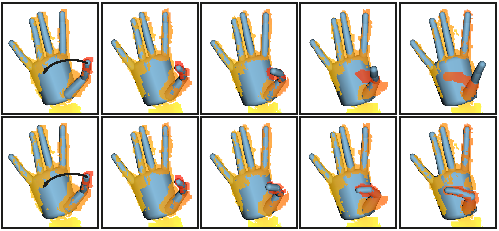
\includegraphics[width=\linewidth]{htrack/fig/teaser/composite.pdf}
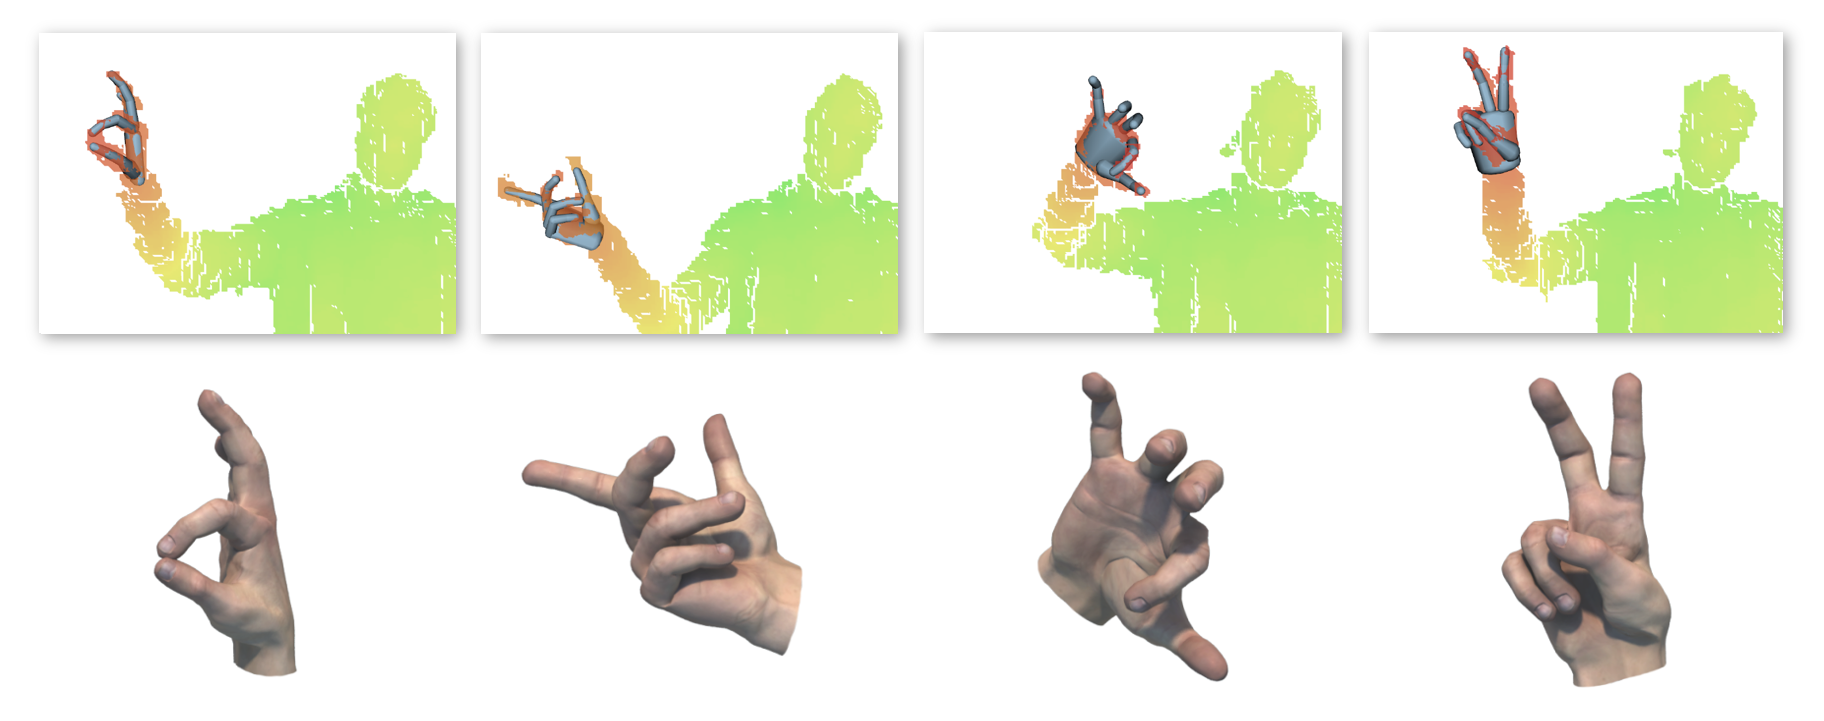
\includegraphics[width=\linewidth]{htrack/fig/teaser/teaser.png}
\centering
\caption{Our system tracks the motion of hands while remaining robust to fast motion, sensor imperfections and self-occlusions.}
% \label{fig:teaser}
\end{figure}
\begin{abstract}
We present a robust method for capturing articulated hand motions in realtime using a single depth camera. Our system is based on a realtime registration process that accurately reconstructs hand poses by fitting a 3D articulated hand model to depth images.
%--- what do we do
We register the hand model using depth, silhouette, and temporal information. To effectively map low-quality depth maps to realistic hand poses, we regularize the registration with kinematic and temporal priors, as well as a data-driven prior built from a database of realistic hand poses.
%--- priors
We present a principled way of integrating such priors into our registration optimization to enable robust tracking without severely restricting the freedom of motion.
%--- correspondences
A core technical contribution is a new method for computing tracking correspondences that directly models occlusions typical of single-camera setups.
%--- Source code
To ensure reproducibility of our results and facilitate future research, we fully disclose the source code of our implementation.

% \begin{classification} % according to http://www.acm.org/class/1998/
% \CCScat{Computer Graphics}{I.3.7}{Three-Dimensional Graphics and Realism}{Animation}
% \CCScat{Information interfaces and presentation}{I.3.7}{User Interfaces}{Input devices and strategies}
% \end{classification}
\end{abstract}



\brief{compare: appearance}
% We demonstrate how our geometric registration achieves accuracy comparable to the state-of-the-art appearance based approaches for tracking hands in isolation, while outperforming them in tracking situations when the hand is not isolated from other elements in the scene.
\brief{compare: model based}
%We also demonstrate the substantial increase in robustness of our method when compared to recently proposed registration-based techniques.
% \MP{I would be less specific here, it sounds a bit defensive. Maybe just say: A core technical contribution is a new method to compute correspondences for tracking. (Maybe add something else, e.g. how we integrate the prior, etc.) We demonstrate how these innovations lead to significant improvements in tracking accuracy in robustness compared to existing solutions (we don't have to be precise as to which ones). 


\begin{figure}[t]
\centering
\begin{overpic} 
[width=\linewidth]
% [width=\linewidth,grid,tics=5]
{htrack/fig/data/composite.pdf}
\put(55,2){$\PointsSensorHtrack$}
\put(55,21){$\PointsSensorHtrack$}
\put(75,2){$\PointsSensorHtrack$}
\put(75,21){$\PointsSensorHtrack$}
\put(95,2){$\SilhoSensor$}
\put(95,21){$\SilhoSensor$}
\putfilename
\end{overpic}
\caption{
%
The two different sensors used in our experiments provide data with substantially different characteristics. Top: Intel's Creative Interactive Gesture camera (time of flight) provides a complete silhouette image \revision{$\SilhoSensor$}, but low quality depth measurements, resulting in severe noise in the point cloud \revision{$\PointsSensorHtrack$}. Bottom: Point clouds acquired by the PrimeSense camera (structured light) are much smoother, but the silhouette image can contain significant gaps.
\vspace{-.2in}
% 
} % caption
\label{fig:data}
\end{figure}

\section{Introduction} \label{sec:htrack-intro}

\brief{why is the problem important}
Tracking and animating humans in motion is a fundamental problem in computer graphics and computer vision. A particularly important question is how to accurately reconstruct the shape and articulation of human hands. Hand motion is a crucial component of non-verbal communication, plays an important role in the animation of humanoid avatars, and is central for numerous human-computer interfaces. 

Accurate realtime body tracking~\cite{shotton_cvpr11,wei_siga12} and face tracking~\cite{cao_sig14} systems have been recently proposed. Hand tracking is now gaining traction in the research community as a next natural step towards a complete system for online human communication in desktop environments~\cite{oiko2011hand,melax2013dynamics,sridhar2014anisotropic,schroder2014real,tompson2014real}.

Recent industrial trends in interaction systems for virtual environments have lead to the development of (closed source) software packages for the processing of RGBD data, like the Intel RealSense SDK, or purpose-designed hardware, like the Leap Motion and the Nimble sensors. 

\brief{why other approaches suck}

In this paper we introduce a system for \emph{realtime} hand tracking suitable for personal desktop environments. Our \emph{non-invasive} setup using a single commodity RGBD~sensor does not require the user to wear a glove or markers. 
Such single-camera acquisition is particularly advantageous as it is cheap, does not require any sensor calibration, and does not impede user movements. 

\brief{why is it still challenging}
Accurate hand tracking with a non-invasive sensing device in realtime is a challenging scientific problem. Human hands are highly articulated and therefore require models with sufficiently many degrees of freedom to adequately describe the corresponding motion space. Hand motion is often fast and exhibits intricate geometric configurations with complex contact patterns among fingers. 

With a single-camera RGBD setup, we are faced with incomplete data due to self-occlusions and high noise levels (see Figure~\ref{fig:data}).

Yet the simplicity of the hardware and the ease of deployment make this setup the most promising for consumer applications as evidenced by the recent proliferation of new consumer-level sensors.

To cope with the limited amount of available information, we employ an articulated template model as a geometric prior for shape completion and topology control. Our model does not only encode geometry, but also serves as a domain to represent information about \emph{plausible} hand poses and motions. This statistical information, built by analyzing a database of annotated poses, is directly embedded into the optimization, which
allows accurate tracking with a high number of degrees of freedom even in challenging scenarios.

\subsection*{Contributions}
% 
We present a complete system for realtime hand tracking using a single commodity RBGD input sensor. Our core technical contributions are:
% 
\begin{figure}[t]
\centering
\begin{overpic} 
[width=\linewidth]
% [width=\linewidth,grid,tics=5]
% {fig/handmodel/composite.png}
{htrack/fig/handmodel/composite.pdf}
\put(36,1){\small $\skelpoint_0$}
\put(38,9){\small $\skelpoint_1$}
\put(40,14){\small $\skelpoint_2$}
\put(42.5,19.5){\small $\skelpoint_3$}
\put(43.5,23){\small $\skelpoint_4$}
% Too cluttered if we put more!!!
\putfilename
\end{overpic}
\caption{ 
%
A visualization of the template hand model with the number and location of degrees of freedom of our optimization. From left to right: The cylinder model used for tracking, the skeleton, the BVH skeleton exported to Maya to drive the rendering, the rendered hand model. 
% Note the rig bones of fingertips are sligthly longer, as they extend until they touch the surface.
% \MP{Not sure if I understand the last sentence. Should we skip it?}
%\TODO{Replace (d) with posed rendered model.}
} % caption
\label{fig:handmodel}
\end{figure}


\begin {itemize}
\item \new{a novel articulated registration algorithm that efficiently integrates data and regularization priors into a \emph{unified} real-time solver; see \Section{optimization} and \Appendix{gpu},}
\item a combined 2D/3D registration method to align the 3D hand model to the acquired depth map and extracted silhouette image; see \Section{fitting},
\item a new way of computing data-to-model correspondences that accounts for occlusions and significantly improves the robustness of the tracking; see \Section{fitting},
\item a new regularization strategy that combines a statistical pose-space prior with kinematic and temporal priors to \new{simultaneously} ensure the inferred hand poses are plausible
%--- This is about the PCA-mean discussion we had in the rebuttal.
\new{and aid the algorithm in recovering from loss-of-tracking; see \Section{prior},}
\item \new{exposing an interesting relationship between the well known point-to-plane registration energy and Gauss-Newton linearization;  
see \Appendix{lindistance}.}
\end{itemize}

Another important contribution of our paper is that we fully disclose our source code\footnote{\url{https://github.com/OpenGP/htrack}}. To the best of our knowledge, no other freely available implementation is available, and we believe that publishing our code will not only ensure reproducibility of our results, but also facilitate future research in this domain.

\new{Note that there is a widespread belief \cite{wei_siga12,zhang_siga14,qian2014realtime} that ICP-like techniques are too local and prone to local minima to successfully deal with fast articulated motion. One of our contributions is to show this commonly held belief should be re-considered. We demonstrate that a regularized geometric registration approach in the spirit of ICP can achieve outstanding performance. We believe this will significantly impact future research in this domain, as it will allow further development of registration techniques for real-time tracking, in contraposition to commonly employed techniques from the vision community like  discriminative~\cite{tompson2014real} and PSO~\cite{qian2014realtime} methods.}

Our regularized geometric registration achieves robust, highly articulated hand tracking at up to 120 frames per second (fps).
%
We quantitatively and qualitatively compare the performance of our algorithm to recent appearance-based and model-based techniques (see \Section{eval}). These comparisons show a significant improvement in accuracy and robustness compared to the current state-of-the-art.

% !TEX root = ../../thesis.tex

\begin{figure*}[t]
\centering
\begin{overpic} 
[width=\linewidth]
% [width=\linewidth,grid,tics=5]
{htrack/fig/overview/composite.pdf}
\put(92.5,19.3){\small{$\parsHtrack(t)$}}
%\put(83.5,18.6){\small{$\delta(t-2)$}}
%\put(83.5,20.25){\small{$\delta(t-1)$}}
\put(63.0,4){\small{$[\underline\parsHtrack,\overline\parsHtrack]$}}
\putfilename
\end{overpic}
\caption{
% 
Overview of our algorithm. For each acquired frame we extract a 3D point cloud of the hand and the 2D distance transform of its silhouette. 
% 
From these we compute point correspondences to align a cylinder model of the hand to best match the data. This registration is performed in an ICP-like optimization that incorporates a number of regularizing priors to ensure accurate and robust tracking.
%fit our hand model to the data. In an ICP fashion, these correspondences are computed using the cylinder model posed and the silhouette image of from the previous solver iteration.
% 
%A number of priors regularize tracking, amongst which the result of previously tracked frames. Our solver optimizes for both joint angles and global transformation of a skeletal hand model.}
}
\label{fig:overview}
\end{figure*}

\section{Related Work}
\label{sec:htrack-related}


\subsection*{Appearance-based hand tracking} 
 
As discussed in Chapter \ref{thesis_intro} numerous appearance-based methods have been developed for hand tracking. 
The strength of these methods is the capability of inferring a hand pose from a single frame without the need of relying on temporal coherence, which avoids drift.
 However, such appearance-based approaches are tightly linked to the training data and often do not generalize well to previously unseen hand poses, i.e., poses not contained in the training database. For this reason most of these methods assume a single hand in isolation to avoid data explosion, and often do not reach the accuracy of model-based methods.

\subsection*{Model-based hand tracking}

A popular approach to hand motion capture is to use a marker-based system (e.g.\ Vicon, OptiTrack).  A 3D hand model can then be fitted to the tracked markers to get the final hand poses. A small number of markers has been shown to be sufficient for reconstructing the 3D hand poses via inverse kinematics techniques~\cite{Hoyet_i3d12}. However, due to frequent occlusions of the markers, motion sequences acquired using marker-based systems often need a significant amount of manual cleaning. To overcome this issue, \cite{zhao2012marker} propose to complement a marker-based system with RGBD data to capture hand motion even in case of significant self-occlusion.
Recently, accurate model-based tracking has been achieved in a multiple camera setup~\cite{sridhar2013multicam,sridhar2014anisotropic}, where the multiple vantage points help resolving challenging occlusions. Multiple camera systems have also been used successfully to model precise hand-hand and hand-object interactions~\cite{oiko_iccv11,ballan2013salient,wang2013physics}. All of the above methods require a complex acquisition setup and manual calibration, which makes them less suitable for the kind of consumer-level applications that we target with this work.

\emph{Particle-swarm optimization} (PSO) methods achieve interactive (15~fps) tracking with a single RGBD camera~\cite{oiko2011hand}. PSO techniques have also been applied successfully to model challenging interaction between two hands \cite{oiko_cvpr12} at a reduced rate of 4 fps. 
PSO is an optimization heuristic that does not use the gradient information of the considered optimization problem, but instead uses a sampling strategy.
For this reason the accuracy and efficiency of PSO approaches heavily rely on the number of samples used. Oikonomidis et al.~\cite{oikonomidis2014evolutionary} introduced a more advanced sampling strategy that improves tracking efficiency without compromising quality. However, gradient-based optimization approaches  converge faster and more accurately than PSO when close to the solution, and are therefore well suited for realtime applications~\cite{qian2014realtime}.


Compelling 60 fps realtime performance was recently shown using gradient-based optimization by~\cite{melax2013dynamics}, where the optimization is expressed as a convex rigid body simulation, and numerous heuristics for re-initialization were employed to avoid tracking failures. Rather than resorting to reinitialization for robustness, \cite{schroder2014real} formulate the optimization in a subspace of likely hand poses. While the lower number of optimization variables leads to efficient computations, tracking accuracy can be limited by the reduced pose complexity induced by the subspace.

 In this paper, we show that hand tracking can be formulated as a single gradient-based optimization to obtain an efficient and accurate real-time tracking system running at up to 120 fps. By using a combination of geometric and data-driven priors we achieve significant improvements in tracking quality and robustness.

%% !TEX root = ../htrack.tex
\section{Overview}
% - input data from sensors, illustrate how the data sucks
% - our hand model, motivation of why we use the cylinders
% - output, i.e. pose parameters
% - short paragraphs on the registration formulation and the optimization
% - highlight contributions again
Robust hand tracking with a commodity depth sensor is highly challenging due to self-occlusion, low quality/density of sensor data and the high degree of articulation of the human hand.
We address these issues by proposing a regularized articulated ICP-like optimization that carefully balances data fitting with suitable priors (\Figure{overview}). 
%
Our data fitting performs a joint \emph{2D-3D} optimization. 
% \MP{Would be good to add an overview figure that shows the different components and notation. Input data, preprocessing, registration optimization with different terms, data prior, output data.}
The 3D alignment ensures that every point measured by the sensor is sufficiently close to the tracked model $\handmodel$.
% \MP{We should be consistent about notation. Later, $\PointsSensor$ is a point cloud, here it looks like it's the sensor or a point from the sensor. It's probably easiest not to introduce the notation in this paragraph.}
Simultaneously, as we cannot create such constraints for occluded parts of the hand, we integrate a 2D registration that pushes the tracked model to lie within the sensor visual hull. A carefully chosen set of priors regularizes the solution to ensure the recovered pose is plausible. 

% We determined that retaining realistic hand postures is critical, as erroneous postures can result in establishing erroneous closest-point correspondences and cause catastrophic loss of tracking. \MP{not clear to me. a realistic pose can just as well lead to wrong correspondences. I would probably skip this sentence.}


\paragraph*{Acquisition device.}
Our system processes raw data acquired at 60 fps from a single RGBD sensor. \Figure{data} illustrates this data for the \emph{PrimeSense Carmine 1.09} structured light sensor as well as the \emph{Creative Gesture Camera} time-of-flight sensor. From the raw data our algorithm extracts a 2D \emph{silhouette image} $\SilhoSensor$ and a 3D \emph{point cloud} $\PointsSensor$. The two sensors exhibit different types of imperfections. The precision of depth measurements in the PrimeSense camera is significantly higher. However, substantial holes often occur at grazing angles, e.g.\ note the gap in the data where we would expect to see the index finger. Conversely, the Creative Gesture Camera provides an accurate and gap-free silhouette image, but suffers from high noise in the depth measurements, therefore resulting in very noisy point clouds. Our algorithm is designed to handle both types of imperfections. This is achieved by formulating an optimization that \emph{jointly} considers silhouette and point cloud, balancing their contribution in a way that conforms to the quality of sensor data.

\begin{figure}[t]
\centering
\begin{overpic} 
[width=\linewidth]
% [width=\linewidth,grid,tics=5]
% {fig/wristband/composite.pdf}
{htrack/fig/wristband/composite.png}
% \put(0,0){\small{text}}
\put(75,02){\tiny{sensor cloud}$\PointsSensor$}
\put(75,22){\tiny{sensor silh.} $\SilhoSensor$}
\put(1,02){\tiny{wristband mask}}
\put(1,22){\tiny{depth image}}
\put(30,02){\tiny{PCA wristband}}
\put(53,02){\tiny{hand ROI}}
\put(35.5,17){$\ell$}
\putfilename
\end{overpic}
\caption{
% \todo{[wristband]}
%
We first identify the wristband mask by color segmentation, then compute the 3D orientation of the forearm as the PCA axis of points in its proximity.
Offsetting a 3D sphere  from the wristband center allows isolating the region of interest. The obtained silhouette image and sensor point clouds are shown on the right. 
\vspace{-.2in}
% \TODO{display padding sensor silhouette}
% 
}
\label{fig:wristband}
\end{figure}



\paragraph*{Tracking model.}
Our algorithm registers a template hand model to the sensor data. Similar to other techniques~\cite{oiko_bmvc11,schroeder_icra14}, we employ a simple (sphere capped) cylinder model as a geometric template; see \Figure{handmodel}.  We optimize for $26$ degrees of freedom, $6$ for global rotation and translation and $20$ for articulation.
% 
% \MP{We should say something about how the hand is customized to the user. Right now, it appears as if one generic model would work for all people.}
Like in \cite{melax_13}, the model can be quickly adjusted to the user by specifying global scale, palm size and finger lengths. In most scenarios, it is sufficient to perform a simple uniform scaling of the model.
% 
Such a coarse geometry is sufficient for hand tracking, as the signal-to-noise ratio for commercially available RGBD sensors is low for samples on the fingers when compared to the size of a finger. Furthermore, the computation of closest-point correspondences can be performed in closed form and in parallel, which is essential for real-time performance.
% 
\revision{The hand's palm region may be better approximated by geometries other than a cylinder, but we found using only cylinder primitives to work well for tracking in terms of accuracy and efficiency. Furthermore, it simplified the implementation as the same correspondence computation routine can be used for all primitives in the model.}
% 
While the geometry of the model used for tracking remains coarse, our algorithm computes joint angles (including rigid transformation) in the widespread \emph{BVH} motion sequence format; these can be used to drive a high-resolution skinned hand rig as illustrated in \Figure{handmodel}-d.
%

%\section{Technical details}
\label{sec:tech}
\paragraph*{Preprocessing.}
The  silhouette image $\SilhoSensor$ is not directly available from the sensor and needs to be computed. This labeling can be obtained by extracting  the sensor color image and performing a skin color segmentation~\cite{oiko_cvpr12,schroeder_icra14}, or can be obtained directly from depth images by performing a classification with randomized forests~\cite{tompson_tog14}. Another possibility is to exploit a full-body tracking algorithm~\cite{shotton_cvpr11} and segment the hand according to the wrist position. For gestural tracking, where the hand is typically the closest object to the sensor~\cite{qian_cvpr14}, a black wristband can be used to simplify segmentation by creating a gap in the depth image. Similarly to this method, in our system the user wears a \emph{colored wristband}. We first identify the position of the wristband in the scene by color segmentation,
then retrieve the 3D points in the proximity of the wristband and compute the principal axis. This axis, in conjunction with the wristband centroid, is then used to segment the hand point cloud. Any depth pixel within the hand point cloud is labelled as belonging to the silhouette image $\SilhoSensor$ as shown in \Figure{wristband}.
% \MP{We should add an image here.} DONE



%%% Local Variables:  
%%% mode: latex 
%%% TeX-master: "../htrack" 
%%% End: 

%% !TEX root = ../../thesis.tex


\begin{figure}[t]
\flushleft
\begin{overpic} 
[width=\linewidth]
% [width=.97\linewidth,grid,tics=5]
{htrack/fig/frontcorr/composite.pdf}
\put(98, 1){\tiny\rotatebox{90}{Converged}}
\put(98,18.7){\tiny\rotatebox{90}{First Iter.}}
\put(98,34.7){\tiny\rotatebox{90}{Initial.}}
\put(15,-3){\small(a)}
\put(43,-3){\small(b)}
\put(78,-3){\small(c)}
\put(9,32){\tiny$\PointsSensor$}
\put(25,43){\tiny$\handmodel$}
\put(17,37){\color{red}$\proj_\handmodel$}
\put(45,37){\color{red}$\proj_\handmodel$}
\put(73,37){\color{red}$\proj_{\visiblehand}$}
\putfilename
\end{overpic}
% \vspace{-.05in}
\caption{
% 
Illustration of correspondences computations. The circles represent cross-sections of the fingers, the small black dots are samples of the depth map. (a) A configuration that can be handled by standard closest point correspondences.
 (b) Closest point correspondences to the back of the cylinder model can cause the registration to fall into a local minimum. Note that simply pruning correspondences with back-pointing normals would not solve this issue, as no constraints would remain to pull the finger towards the data. (c) This problem is resolved by taking visibility into account, and computing closest points only to the portion $\visiblehand$ of $\handmodel$ facing the camera. % 
}
\label{fig:frontcorr}
\end{figure}

\section{Optimization}
\label{sec:optimization}
In this section we derive the objective functions of our model-based optimization method
and provide the rationales for our design choices. 
Let $\DataSensor$ be the sensor input data consisting of a 3D point cloud $\PointsSensorHtrack$ and 2D silhouette $\SilhoSensor$ (see \Figure{data}). Given a 3D hand model $\handmodel$ with joint parameters $\parsHtrack = \{ \theta_1, \theta_2,\hdots, \theta_{26} \}$, we aim at recovering the pose $\parsHtrack$ of the user's hand, matching the sensor input data $\DataSensor$. 
To achieve this goal, we solve the optimization 
problem
% 
%\begin{equation}
%\label{eq:tracking_optimization}
%\argmin_{\pars} E_{\text{fit}} + E_{\text{prior}},
%\end{equation}
%
\begin{equation}
\label{eq:tracking_optimization}
\min_{\parsHtrack} \:\: \underbrace{E_{\text{3D}} + E_{\text{2D}} \new{+ E_{\text{wrist}}}}_{\text{Fitting terms}} + \underbrace{E_{\text{pose}} + E_{\text{kin.}} + E_{\text{temporal}}}_{\text{Prior terms}},
\end{equation}
%
combining fitting terms that measure how well the hand parameters~$\parsHtrack$ represent the data frame $\DataSensor$, with prior terms that regularize the solution to ensure realistic hand poses. For brevity of notation we omit the arguments $\parsHtrack, \PointsSensorHtrack,\SilhoSensor$ of the energy terms. We first introduce the fitting terms and present our new solution to compute tracking correspondences. Then we discuss the prior terms and highlight their benefits in terms of tracking accuracy and robustness. 
%
More details on the  implementation of the optimization algorithm will be given in \Section{implementation} and the appendix.

\begin{figure}[t]
\centering
\begin{overpic} 
[width=\linewidth]
% [width=\linewidth,grid,tics=5]
{htrack/fig/occlusion/composite.pdf}
\put(22,-1){\small(a)}
\put(53,-1){\small(b)}
\put(85,-1){\small(c)}
\put(18,14){$c_1$}
\put(49,14){$c_1$}
\put(80,14){$c_1$}
\put(32,6){$c_2$}
\put(63,14){$c_2$}
\put(94,14){$c_2$}
\putfilename
\end{overpic}
\vspace{1em}
\caption{
% We illustrate the necessity to compute correspondences against
% 
Illustration of the impact of self-occlusion in correspondences computations. 
(a) The finger $c_2$ initially occluded by finger $c_1$ becomes visible, which causes new samples to appear. (b)  Closest correspondences to the portion of the model visible from the camera do not generate any constraints that pull $c_2$ toward its data samples. This is the approach in \protect\cite{wei_siga12}, where these erroneous matches are then simply pruned. (c) Our method also considers front-facing portions of the model that are occluded, allowing the geometry to correctly register.      
%
}
\label{fig:occlusion}
\end{figure}

\subsection{Fitting Energies}
\label{sec:fitting}


%\begin{figure}[t!]
\centering
\begin{overpic}
[width=\linewidth]
% [width=\linewidth,grid,tics=10]
{\currfiledir/item.pdf}
\put(1,30){{\small$\%$}}
\put(1,64){{\small$\%$}}
\put(93,37.5){{\small $E_{3D}$}}
\put(93,04.5){{\small $E_{2D}$}}
\end{overpic}
\caption{
% 
%
\todo{Each plot visualizes on the $y$ axis the portion of frames with a mean error metric below the value reported on the $x$ axis. We employ the \handyseq{teaser} sequence for this purpose. Curves closer to the top-left quadrant indicate better performance.}
% 
% Our method is quantitatively compared to the one of~\protect\cite{tagliasacchi2015robust} on the \handyseq{teaser} sequence.
% 
% 
}
\label{fig:comp2}
\end{figure}
\section{Calibration}
\label{sec:modeling}

\brief{Multi-Pose Data}
Our calibration procedure adapts our template model to a specific user from a set of $N$ 3D measurements $\{ \depth_1 \dots \depth_N \}$ of the user's hand in different poses. Multiple measurements are necessary, as it is not possible to understand the kinematic behavior by analyzing static geometry, and the redundancy of information improves fitting precision. Further, in  monocular acquisition this redundancy is essential, as single-view data is highly incomplete\todo{,} making the problem ill-posed. In our research we have experimented with datasets $\{\depth_n\}$ acquired via multi-view stereo (e.g. \emph{Agisoft Photoscan}), as well as a single RGBD sensor. 
Our calibration formulation can be employed for both acquisition modalities.
\todo{Dynamic reconstruction frameworks such as~\cite{newcombe2015dynfusion} or \cite{innmann2016volume} could also be used to generate a dynamic template mesh over which sphere-mesh decimation could be executed~\cite{thiery2016spheremesh}. 
However, as no public implementation is currently available, it is currently unclear how well these methods would cope with loop-closure for features as small as human fingers.}

\subsection*{Kinematics}
The rest-pose geometry of our model is fully specified by two matrices specifying the set of sphere positions $\restcenters$ and \todo{the set of} radii $\radii$. The geometry is then posed through the application of  kinematic chain transformations; see \Figure{posing}a. Given a point $\bar\pointHmodel$ on the model $\model$ at rest pose, its 3D position after posing can be computed by evaluating the expression:
% 
\begin{equation}
\pointHmodel = \left[ \Pi_{k \in K(\bar\pointHmodel)} \mathbf{\bar{T}}_k \mathbf{T}_k \mathbf{\bar{T}}_k^{-1} \right] \bar\pointHmodel
\label{eq:kinematic}
% we apply the posing transformation, then we re-apply the rest pose transformation to bring the point back in world coordinates
\end{equation}
%
where $\mathbf{T}_*$ are the \emph{pose} transformations parameterized by $\parpose$ and $\Pi$ left multiplies matrices by recursively traversing the kinematic chain $K$ of point $\bar\pointHmodel$ towards the root~\cite{buss2004introduction}. 
Each node $k$ of the kinematic chain is associated with an orthogonal frame $\mathbf{\bar{T}}_k$ according to which local transformations are specified. In most tracking systems, the frames $\mathbf{\bar{T}}_*$ are manually set by a 3D modeling artist and kept fixed across users. However, incorrectly specified kinematic frames can be highly detrimental to tracking quality; see \Figure{posing}(c,d) and \VideoKinematic{}. Therefore, in our formulation, the kinematic structure (i.e. the matrices $\mathbf{\bar{T}}_*$) is directly optimized from acquired data.

\begin{figure}[t!]
\centering
\begin{overpic} 
[width=\linewidth]
% [width=\linewidth,grid,tics=10]
{\currfiledir/item.pdf}
\put(93,37.5){{\small $E_{3D}$}}
\put(93,04.5){{\small $E_{2D}$}}
\put(1,30){{\small $\%$}}
\put(1,64){{\small $\%$}}
\end{overpic}
\caption{\todo{Calibrating progressively improves the 2D/3D tracking metrics, showing a remarkable improvement in tracking fidelity from~\protect\cite{tagliasacchi2015robust} to~\citeme{}.}}
\label{fig:calibeval}
\end{figure}
\begin{figure*}[h!]
\centering
\begin{overpic} 
[width=\linewidth]
% [width=\linewidth,grid,tics=10]
{hmodel/fig/calibration/item.pdf}
% \put(10,10){\todo{\Large Overlay Text}}
\end{overpic}
\caption{
% 
% 
A visualization of a few iterations of our calibration optimization procedure; see \VideoMVS{}. Each quadrant displays a data frame $\depth_n$, $n=1 \dots 4$. Within each quadrant we show three iterations of the optimization. The model being calibrated here is the one employed for real-time tracking in \VideoTeaser{}.
% 
% 
}
\label{fig:calibration}
\end{figure*}

% \newpage
\subsection*{Formulation}
Let $\parpose_n$ be the \emph{pose} parameters optimally aligning the rest-pose template to the data frame $\depth_n$, and $\parposture$ be the \emph{posture} parameters representing the transformations $\mathbf{\bar{T}}_*$ via Euler angles. 

For notational brevity, we also define $\parsHmodel_n=[\parpose_n, \parposture, \restcenters, \radii]$. Our calibration optimization can then be written as:
% 
\begin{eqnarray}
% \parposture, \centers, \radii =
\argmin_{\{\parsHmodel_n\}}
\sum_{n=1}^N 
\sum_{\mathcal{T} \in \termscalib} 
w_\mathcal{T} E_\mathcal{T}(\depth_n, \parsHmodel_n)
\label{eq:calibration}
\end{eqnarray}
% 
We employ a set of energies $\termscalib$ to account for different requirements. On one hand we want a model that is a good fit to the data; on the other, we seek a non-degenerate sphere-mesh template that has been piecewise-rigidly posed. The following calibration energies $\termscalib$ encode these requirements:
% 
\begin{description}[labelsep=0em,labelwidth=.4in,labelindent=1cm,itemsep=-.6em]
\item[d2m] data to model distance
\item[m2d] model to data distance
\item[rigid] elements are posed rigidly
\item[valid] elements should not degenerate
\end{description}
% 
To make this calibration more approachable numerically, we rewrite \Eq{calibration} as an alternating optimization problem:
% 
\begin{eqnarray}
% \restcenters, \radii, \posedcenters =
\argmin_{\posedcenters, \restcenters, \radii} &
\sum_{n=1}^N 
\sum_{\mathcal{T} \in \termscalib}
w_\mathcal{T} E_\mathcal{T}(\depth_n, \centers_n, \restcenters, \radii)
\label{eq:step1}
\\
% \parposes, \parposture =
\argmin_{\parposes,\parposture} &
\sum_{n=1}^N 
\sum_{\mathcal{T} \in \termscalib}
w_\mathcal{T} E_\mathcal{T}(\centers_n, \parsHmodel_n) 
\end{eqnarray}
% 
\todo{Our first step adjusts rest-pose sphere centers $\restcenters$ and radii $\radii$,} by allowing the model to fit to the data without any kinematic constraint beyond rigidity, and returning as a side product a set of \emph{per-frame} posed centers $\posedcenters$. 
Our second step takes the set $\posedcenters$ and projects it onto the manifold of kinematically plausible template deformations. 
This results in the optimization of the rotational components of rest-pose transformations $\mathbf{\bar{T}}_*$, as their translational components are simply derived from $\restcenters$.

\subsection*{Optimization}
The energies above are non-linear and non-convex, but can be optimized offline, as real-time tracking only necessitates a pre-calibrated model. For this reason, we conveniently employ the $lsqnonlin$ Matlab routine, which requires the gradients of our energies as well as an initialization point.
The initialization of $\restcenters$ is performed automatically by anisotropically scaling the vertices of a generic template to roughly fit the rest pose. The initial transformation frame rotations $\parposture$ are retrieved from the default template, while $\parposes$ are obtained by either aligning the scaled template to depth images, or by executing inverse kinematics on a few manually selected keypoints (multi-view stereo).
% 
% \AnastasiaComment{We should say that we use our tracking system with automatically scaled model to get the initial poses. Because the initial poses for calibration from sensor data are extremely close to the final ones. The model will not align to the from the rest pose, only tracking can do this. AT: I already wrote that, the sentence ``aligning the scaled template to the depth images''}
% 
Our (unoptimized) Matlab script calibrates the model within a few minutes for all our examples.


\subsection{Energies}
Our fitting energies are analogous to the ones used in tracking. They approximate the symmetric Hausdorff distance, but they are evaluated on \todo{a \emph{collection} of $N$ frames}:
% 
\begin{eqnarray}
E_{d2m} = 
\sum_{n=1}^N |\depth_n|^{-1} 
\sum_{\pointHmodel \in \depth_n} 
\| \pointHmodel - \proj_{\model(\parsHmodel_n)}(\pointHmodel)\|_2^1 \\
E_{m2d} = 
\sum_{n=1}^N |\model(\parsHmodel_n)|^{-1} 
\sum_{\pixelHmodel \in \model(\parsHmodel_n)} 
\| \pixelHmodel - \proj_{\depth_n}(\pixelHmodel)\|_2^1
\end{eqnarray}
% 
Note that the projection operator $\proj_{\depth_n}$ changes according to the type of input data. If a multi-view acquisition system is used to acquire a complete point cloud, then the projection operator fetches the closest point to $\pointHmodel$ in the point cloud of frame $\depth_n$. If $\depth_n$ is acquired through monocular acquisition, then $\proj_{\depth_n}$ computes the 2D projection to the image-space silhouette of the model.

\subsection*{Rigidity}
It is essential to estimate a \todo{single user template that, once articulated,} \emph{jointly} fits the set of data frames $\{ \depth_n \}$. For this purpose we require each posed model to be a piecewise-rigid articulation of our rest pose. \todo{This can be achieved by constraining each segment $\{ (\ballcenter_{n,i}, \ballcenter_{n,j})\:|\: ij \in \skeletonHmodel \}$ of $\centers_n$ to have the same length as the corresponding segment $(\bar\ballcenter_i, \bar\ballcenter_j)$ of the rest pose configuration $\restcenters$}:
% 
\begin{equation}
E_{\text{rigid}} = 
% \sum_{\ballcenter_{n,*} \in \centers_n}
\sum_{ij \in \skeletonHmodel} (\| \ballcenter_{n,i} - \ballcenter_{n,j} \| - \| \bar\ballcenter_i - \bar\ballcenter_j \|)^2
\end{equation}
% 
Note that only a subset of the edges of our control skeleton, as illustrated in \Figure{topology}, are required to satisfy this rigidity condition.

% \newpage
\subsection*{Validity}
The calibration optimization should avoid producing degenerate configurations \todo{in our \emph{rest pose} template $\restcenters$}. For example, a pill degenerates into a sphere when one of its balls is fully contained within  the volume of the other. Analogously, a wedge can degenerate into a pill or a sphere. We monitor validity by an indicator function $\chi(\bar\ball_i)$ that evaluates to one if $\bar\ball_i$ is degenerate and zero otherwise.
% 
\todo{We make a conservative choice and use $\chi(\bar\ball_i)$, which verifies whether $\bar\ballcenter_i$ is inside $\bar\oneelement \setminus \bar\ball_i$, the element obtained by removing a vertex, as well as all its adjacent edges, from $\bar\oneelement$.}
% 
This leads to the following \todo{conditional} penalty function:
% 
\begin{equation}
E_{\text{valid}} = 
\sum_{\bar\oneelement \in \restcenters}
\sum_{\bar\ball_i \in \bar\oneelement} 
\chi(\bar\ball_i) 
\| \bar\ballcenter_i - \proj_{\bar\oneelement \setminus \bar\ball_i}(\bar\ballcenter_i) \|_2^2
\end{equation}
% 
 


%Our fitting energy $E_{\text{fit}}$ captures the alignment of the hand model with the 3D point cloud and the 2D silhouette by combining two distinct energies
%% 
%\begin{equation}
%E_{\text{fit}} =  E_{\text{3D}} + E_{\text{2D}}.
%\label{eq:fitting}
%\end{equation}
%
%
% Our data fitting performs a joint 2D-3D op- timization. Our 3D alignment ensures that every point measured by the sensor Xs is sufficiently close to the tracked model M. Si- multaneously, as we cannot create such constraints for occluded portions of the hand, we optimize for a 2D registration that ensures the tracked M lies in the sensor visual hull Ss. O
%
%
% Our priors regularize the solution to ensure the recovered pose remains likely. We determined that retaining realistic hand postures is critical, as erroneous postures can result in establishing erroneous closest-point correspondences and cause catastrophic loss of tracking.
%


\subsection*{Point cloud alignment}
%The quality of the point cloud alignment is measured using $E_{\text{3D}}$. 
The term $E_{\text{3D}}$ models a 3D geometric registration in the spirit of ICP as
%. The energy is defined as
%
\begin{equation}
    E_{\text{3D}}  = \omegacloud \sum_{\pointHtrack \in \PointsSensorHtrack} \| \pointHtrack - \proj_{\handmodel(\parsHtrack)}(\pointHtrack,\parsHtrack) \|_2^1,
\label{eq:align3d}
\end{equation}
%
where $\|\cdot\|_2$ denotes the $\ell_2$ norm, $\pointHtrack$ represents a 3D point of $\PointsSensorHtrack$, and $\proj_{\handmodel(\parsHtrack)}(\pointHtrack,\parsHtrack)$ is the projection of $\pointHtrack$ onto the hand model $\handmodel$ with hand pose $\parsHtrack$. 
%This projection defines the correspondence of $\point$ on the model. For brevity of notation, we define this correspondence as $\mathbf{y} = \proj_{\handmodel}(\point,\pars)$.
%
 Note that we compute a sum of absolute values of the registration residuals, not their squares. This corresponds to a mixed $\ell_{2}/\ell_{1}$ norm of the stacked vector of the residuals. For 3D registration such a sparsity-inducing norm has been shown to be more resilient to noisy point clouds containing a certain amount of outliers
such as the ones produced by the Creative sensor (\Figure{data}). We refer to~\cite{Bouaziz_eg2014} for more details.

% \SB{not sure if we should say that here: As the 3D hand model is simply composed of cylinders, we compute the projections in close form ignoring back facing correspondences.}


\begin{figure}[t]
\centering
\flushleft
\begin{overpic} 
[width=.97\linewidth]
% [width=.97\linewidth,grid,tics=5]
{htrack/fig/occnrg/composite.pdf}
\put(100,2){\rotatebox{90}{\small{corresp. culling}}}
\put(100,24){\rotatebox{90}{\small{occlusion energy}}}
\putfilename
\end{overpic}
\vspace{1em}
\caption{
% 
Correspondence computations.
The top row shows the strategy 
% originally proposed for full-body tracking by \protect\cite{ganapathi_eccv12}
used in~\protect\cite{qian2014realtime} adapted to our gradient-based framework according to the formulation given in~\protect\cite{wei_siga12}. The bottom row shows the improved accuracy of our new approach.
% 
%The effect of replacing our view-dependent correspondence computation by an energy minimizing depth disparity~\protect\cite{wei_siga12} for portions of the model occluding the sensor data~\protect\cite{qian_cvpr14}. \MP{I don't understand the references. So the top row is Wei et al and the bottom row our method? Why refer to Qian?}
} % caption
\label{fig:occnrg}
\end{figure}

\subsection*{3D correspondences}
% The projection operators are now decoupled from the optimization and can be evaluated, rather than differentiated.
% The optimization problems in Step.1 can be solved in close form. The computation of 3D correspondences in \Equation{cp3d} can be performed either by exhaustively computing the distances to the underlying cylinder model, or by first rendering the point cloud with the same viewport of the sensor and then fetching closest points with a spatial data structure (kdtree or octree). \AT{Note that the first way of computing closest points is trivially parallelizable}
The 3D registration term involves computing the corresponding point  $\mathbf{y} = \proj_{\handmodel(\parsHtrack)}(\pointHtrack,\parsHtrack)$ on the cylinder model~$\handmodel$ for each sensor point $\pointHtrack \in \PointsSensorHtrack$. 
In contrast to standard closest point search, we define the correspondence $\mathbf{y}$  as the closest point on the \emph{front-facing} part $\visiblehand$ of $\handmodel$. This includes parts of the model that are oriented towards the camera but occluded by other parts. 
 In our experiments we learned that this seemingly simple extension proved absolutely essential to obtain high-quality tracking results.
 Only considering model points that are visible from the sensor viewpoint, i.e., matching to the rendered model, is not sufficient for handling occlusions or instances of disappearing and reappearing sensor data; see \Figure{frontcorr} and \Figure{occlusion}. 
 
To calculate $\mathbf{y}$, we first compute the closest points $\pointHtrack_\mathcal{C}$ of $\pointHtrack$ to each cylinder $\mathcal{C}\in\handmodel$. Recall that our hand model consists of sphere-capped cylinders so these closest points can be computed efficiently in closed form and in parallel for each $\pointHtrack \in \PointsSensorHtrack$.
We then identify back-facing points using the dot product of the cylinder surface normal $\mathbf{n}$ at $\pointHtrack_\mathcal{C}$ and the view ray vector $\mathbf{v}$. 
%
For efficiency reasons, we use a simplified orthographic camera model where the view rays are constant, i.e., $\mathbf{v} = [0~0~1]^T$. If a point on a cylinder is back-facing ($\mathbf{n}^T\mathbf{v}>0$), we project $\pointHtrack$ onto the cylinder's silhouette contour line from the camera perspective, whose normals are orthogonal to $\mathbf{v}$.

%We first compute the orthogonal projection of $\point$ onto the cylinder's center line segment. The point on the cylinder's surface is then found by moving back along the projection axis by the cylinder radius.


%As the sensor data only contains points that are visible from the camera's point of view, we only project to the parts of the cylinder that are front-facing with respect to the camera. This includes parts of the model that are oriented towards the camera but occluded by other parts of the model. Only considering model points that are visible from the sensor viewpoint, i.e., matching to the rendered model point cloud, is not sufficient for handling occlusions or instances of disappearing and reappearing sensor data (see \Figure{frontcorr} and \Figure{occlusion}). 



% 
% Conversely, to establish closest point correspondences to $\SilhoSensor$, we first compute its distance transform in linear time using~\cite{felzenszwalb_12} (1ms on a 320x240 image).
 
A different strategy to address visibility issues has been introduced \new{ in~\cite{qian2014realtime}. These methods} propose an energy that penalizes areas of the model falling in front of the data, which is then optimized using particle swarms. This energy can be integrated into our optimization following the formulation in \cite[Eq. 15]{wei_siga12}. However, such an energy is prone to create local minima in gradient-based optimization, as illustrated in \Figure{occnrg}. Here the thumb has difficulty entering the palm region, as it must occlude palm samples before reaching its target~configuration. Our correspondence search avoids such problems.
\new{Furthermore, note how~\cite{qian2014realtime} follows a \emph{hypothesize-and-test} paradigm where visibility constraints in the form of \emph{ray-casting} are easy to include. As discussed in  \cite{ganapathi_eccv12}, such constraints are much more difficult to include in iterative optimization techniques like ours. However, our front-facing correspondences computation provides a simple and elegant way to deal with such shortcomings.}


% takes the energy formulation of~, which was optimized by particle swarm optimization, and adapts it to our gradient-based formulation; see~.

% \MP{Does this make more sense? I would still like to give an explanation of what is happening here. People might not know Qian. Can we say in one sentence what the difference is?}

%\AT{this is a dangerous statement. We implement the energy proposed in \cite{qian_cvpr14} and then linearize it. It's the gradient of this energy that is f'd, but if you follow a particle swarm strategy it does work `ok'}, highlighting the improved tracking accuracy of our approach.

\begin{figure}[t]
\centering
\begin{overpic} 
[width=\linewidth]
% [width=\linewidth,grid,tics=5]
% {fig/push/composite.pdf} %f'd up transparency
{htrack/fig/push/composite.png}
\put(44,40){\small{$\SilhoSensor$}}
\put(44,18){\small{$\SilhoSensor$}}
\put(31.5,-2){\small{silhouette}}
\put(54.5,-2){\small{w/o silhouette}}
\put(79.5,-2){\small{w/ silhouette}}
\putfilename
\end{overpic}
\vspace{1em}
\caption{
% \todo{[push]}
Our 2D silhouette registration energy is essential to avoid tracking errors for occluded parts of the hand.
When no depth data is available for certain parts of the model, a plausible pose is inferred by ensuring that the model is contained within the sensor silhouette image $\SilhoSensor$.
% correctly track occluded geometry. In these scenarios, it is the lack of data of depth measurements in certain areas that drives pose inference - by ensuring our model is behind by the sensor silhouette $\SilhoSensor$.
}
\label{fig:push}
\end{figure}

\subsection*{Silhouette alignment}
The 3D alignment energy $E_{\text{3D}}$ robustly measures the distance between every point in the 3D point cloud~$\PointsSensorHtrack$ to the tracked model $\handmodel$. However, as hands are highly articulated, significant self-occlusions are common during tracking. Such self-occlusions are challenging, because occluded parts will not be constrained when only using a 3D alignment energy. For this reason, we use a 2D silhouette term $E_{\text{2D}}$ that models the  alignment of the 2D silhouette of our rendered hand model with the 2D silhouette extracted from the sensor data as 
%
%The second term $E_{\text{2D}}$ models a 2D geometric alignment in a similar manner than the $E_{\text{3D}}$ energy as
%
\begin{equation}
    E_{\text{2D}} = \omegasilhouette \sum_{\pixelHtrack \in \SilhoRender} \| \pixelHtrack - \proj_{\SilhoSensor}(\pixelHtrack,\parsHtrack) \|_2^2,
\label{eq:align2d}
\end{equation}
%
% where $\pixel$ is a 2D point of the rendered silhouette $\SilhoRender$, and $\proj_{\SilhoSensor}(\pixel,\pars)$ denotes the projection of $\pixel$ onto $\SilhoSensor$.
where $\pixelHtrack$ is a 2D point of the \emph{rendered} silhouette $\SilhoRender$, and $\proj_{\SilhoSensor}(\pixelHtrack,\parsHtrack)$ denotes the projection of $\pixelHtrack$ onto the \emph{sensor} silhouette $\SilhoSensor$.
%over the 2D silhouette extracted from the sensor data $\SilhoSensor$. 
% \SB{not sure if we should say that here: The projections are computed using the 2D distance transform of $\SilhoSensor$~\cite{....}.}
%
\Figure{push} shows why the silhouette term is crucial to avoid erroneous poses when parts of the model are occluded. 
Without the silhouette energy, the occluded fingers can mistakenly move to wrong locations, since they are not constrained by any samples in the depth map.







%\subsection{Correspondence Search}
%
%The 3D and 2D registration energies of Equations~\ref{eq:align3d} and~\ref{eq:align2d} require the computation of point correspondences from the data to the model. Our solution improves upon existing correspondence algorithms without compromising computational efficiency.
%
%



\subsection*{2D correspondences}
In \Equation{align2d}, we compute the silhouette image $\SilhoRender$ by first rendering the hand model $\handmodel$ from the viewpoint of the sensor, caching the bone identifier and the 3D location associated with each pixel in a texture.
% for the computation of the Jacobian in \Equation{jacobian2d} are cached in a texture. 
The projection function $\proj_{\SilhoSensor}(\pixelHtrack,\parsHtrack)$ to compute the
% For each pixels in $\SilhoRender$, we then identify
 closest corresponding point to the sensor silhouette is evaluated efficiently using the 2D distance transform of $\SilhoSensor$.
 We use the linear time algorithm of~\cite{felzenszwalb_12} and store at every pixel the index to the closest correspondence.
% To perform this task efficiently, we compute the 2D distance transform of $\SilhoSensor$ with a linear time algorithm~\cite{felzenszwalb_12}, i.e., at every pixel we store the distance transform value and the index to the closest correspondence.
% simple to evaluate in close form, as they simply require us to compute the closest point to either the tracking model $\handmodel$ or the silhouette of the sensor data $\SilhoSensor$.
% At each iteration we render $\handmodel$ from the viewpoint of the sensor
% We employ the color of each pixel to uniquely identify the originating bone. This information, as well as its 3D position are necessary to compute the gradient of~\Equation{align2d}.
% Step 2 can now be approached by Gauss-Newton optimization; we perform Taylor expansion of the residuals $\mathbf{r}$ of each energy term in \Equation{icp} as $\mathbf{r} \approx \mathbf{r}_0 + \J(\mathbf{r}_0) \delta\pars$, where $\J=\partial \mathbf{r} / \partial \pars$ is the Jacobian of the residuals, and then compute the optimal update as:
% %
% \begin{eqnarray}
% \delta\pars = (\J^t \J + \alpha \mathbf{I})^{-1} \J^t (\mathbf{r} - \mathbf{r_0})
% \label{eq:gaussnewton}
% \end{eqnarray}
% %
% A description of the rows that assemble $\J$, altogether with a description of the chain-rule derivatives is given in the appendix. In the equation above, the term weighted by $\alpha$ both ensures the system remains well conditioned and stabilizes the optimization by reducing the magnitude of the computed update.



% \brief{Convergence Speed}

\begin{figure}[t]
\centering
\begin{overpic} 
[width=\linewidth]
% [width=\linewidth,grid,tics=5]
{htrack/fig/shapespace/composite.pdf}
\putfilename
\end{overpic}
\caption{An illustration of the PCA pose-space used to regularize the optimization. Black dots denote the samples of the data base. 
High likelihood poses are located nearby the mean of the latent space (dark red). 
% Note how the eigenvalues of the PCA space skew the metric in such a way that certain axis offer a broader spectrum of likely poses.
The eigenvalues of the PCA define the metric in the low-dimensional space, skewing it in certain directions. Poses that, according to this metric, are far from the mean are likely to be unnatural and will be penalized in the optimization.
}
\label{fig:shapespace}
\end{figure}

\subsection*{Wrist alignment}
\new{The inclusion of the forearm for hand tracking has been shown beneficial in~\cite{melax2013dynamics}. Our wrist alignment energy encodes a much simplified notion of the forearm in the optimization that enforces the wrist joint to be located along its axis.}
\begin{equation}
    E_\text{wrist} = \omegawrist \| \proj_\text{2D}(\mathbf{k}_0(\parsHtrack)) - \proj_{\ell}(\mathbf{k}_0(\parsHtrack)) \|_2^2,
\end{equation}
\new{
Minimizing this energy helps preventing the hand from erroneously rotating/flipping during tracking; an occurrence of this can be observed at \VideoHtrackWrist \footnote{Please find the accompanying Video1 at \url{http://lgg.epfl.ch/publications/2015/Htrack_ICP/new_video.mp4}
.}.
% 
Here $\mathbf{k}_0$ is the 3D position of the wrist joint, and $\ell$ is the 2D line extracted by PCA of the 3D points associated with the wristband; see \Figure{wristband}. Note that $\proj_\text{2D}$ causes residuals to be minimized in screen-space, therefore the optimization of this energy will be analogous to the one of \Equation{align2d}. 
We optimize in screen space because, due to occlusion, we are only able to observe half of the wrist and this causes its axis to be shifted toward the camera.}

\begin{figure}[t]
\centering
\begin{overpic} 
[width=.8\linewidth]
% [width=.8\linewidth,grid,tics=5]
{htrack/fig/shapespaceproj/composite.pdf}
\put(36,45){$\parsHtrack$}
\put(26,31){$\tilde\parsHtrack$}
\put(26,23){$\boldsymbol{\mu}$}
\put(39,6){$\posespace$}
% \put(25,31){$\tilde\pars$}
\putfilename
\end{overpic}
\caption{
% 
An illustration of the energies involved in our pose-space prior. For illustration purposes the full dimensional parameter vector $\parsHtrack\in\mathbb{R}^3$, while latent space variable $\tilde\parsHtrack\in\mathbb{R}^2$.
% 
The PCA optimization in \protect\cite{schroder2014real} constrains the pose parameters $\parsHtrack$ to lie on the subspace~$\posespace$. Conversely, we penalize the distance of our pose from~$\posespace$~(\Equation{pcaproj}); simultaneously, we ensure our pose remains likely by preventing it from diverging from the mean of the distribution~(\Equation{pcareg}).
% 
% either limiting the freedom of motion of the hand.
% This reduces the freedom of motion, as only poses in the subspace
% This can result in erroneously recovered poses, as $\pars$ can
% 
}
\label{fig:shapespaceproj}
\end{figure}
\begin{figure}[b]
%\flushright
\begin{overpic} 
[width=.98\linewidth]
%[width=.98\linewidth,grid,tics=5]
{htrack/fig/pcaconv/composite_new.pdf}
\put(-1,38){\rotatebox{90}{\tiny{with pose prior}}}
\put(-1,65){\rotatebox{90}{\tiny{w/o pose prior}}}

\put(3.5,4){{\tiny{0}}}
\put(17.6,4){{\tiny{3}}}
\put(31.1,4){{\tiny{6}}}
\put(39.2,4){{\tiny{10}}}

\put(57.4,4){{\tiny{0}}}
\put(71,4){{\tiny{1}}}
\put(84.8,4){{\tiny{2}}}
\put(93.3,4){{\tiny{3}}}

\put(16,0){{\tiny{w/o data term}}}
\put(69,0){{\tiny{with data term}}}
\putfilename
\end{overpic}
\caption{Beyond favoring natural poses, the data prior term also positively affects convergence speed. Top: With the same number of iterations, only with activated data term does the model fully register to the scan. The illustration below shows how the same final state requires significantly fewer iterations with the data term.
}
\label{fig:pcaconv}
\end{figure}
\subsection{Prior Energies}
\label{sec:prior}
Minimizing the fitting energies alone easily leads to unrealistic or unlikely hand poses, due to the deficiencies in the input data caused by noise, occlusions, or motion blur. We therefore regularize the registration with data-driven, kinematic, and temporal priors to ensure that the recovered hand poses are plausible. Each of these terms plays a fundamental role in the stability of our tracking algorithm, as we illustrate below.

%% and is composed of three terms
%% 
%\begin{equation}
%E_{\text{prior}} = E_{\text{pose}} + E_{\text{kinematic}} + E_{\text{temporal}}.
%\label{eq:prior}
%\end{equation}
%%


%The $E_{\text{kinematic}}$ energy aims at generating a plausible hand posture by finding a hand pose respecting some kinematic constraints, i.e., angle bounds and the avoidance of self-collisions. The $E_{\text{temporal}}$ term enforces temporal smoothness to avoid jittering and in order to predict hand parameters in  case of missing data. Finally, to achieve a tracking that produces  postures realizable by a human hand we employ a data-driven energy $E_{\text{pose}}$. 


\subsection*{Pose Space Prior (data-driven)}
\begin{figure}[t]
\centering
\begin{overpic} 
[width=\linewidth]
% [width=\linewidth,grid,tics=5]
{htrack/fig/pca/composite.pdf}
\put(30,-2.5){\small{depth image}}
\put(55,-2.5){\small{without PCA}}
\put(81,-2.5){\small{with PCA}}
\putfilename
\end{overpic}
\vspace{1em}
\caption{
% 
Our pose-space regularization using a PCA prior ensures that a meaningful pose is recovered even when significant holes occur in the input data.
}
\label{fig:pca}
\end{figure}

The complex and highly coupled articulation of human hands is difficult to model directly with geometric or physical constraints. Instead, we use a publicly available database of recorded hand poses~\cite{schroder2014real} to create a data-driven prior $E_{\text{pose}}$ that encodes this coupling.
% To achieve a tracking that produces hand postures which are realizable by a human hand (e.g. we cannot bend a finger on itself), we employ a data-driven regularizer. As a simple example, it is difficult to bend the \emph{distal phalanx} without simultaneously bending the \emph{proximal phalanx}.
We construct a low-dimensional subspace of plausible poses by performing dimensionality reduction using PCA (see \Figure{shapespace}). 
% 
%\begin{eqnarray}
%E_{\text{pose}} = E_{\text{projection}} + E_{\text{mean}}.
%\end{eqnarray}
%
We enforce the hand parameters~$\parsHtrack$ to lie close to this low-dimensional linear subspace using a 
 data term
$E_{\text{pose}} = E_{\text{projection}} + E_{\text{mean}}$.
%
To define the data term, we introduce auxiliary variables $\parssub$, i.e, the PCA weights, representing the (not necessarily orthogonal) projection of the hand pose $\parsHtrack$ onto the subspace; see \Figure{shapespaceproj}.
%\MB{If $\parssub$ is the projection of $\pars$ to the PCA space, then it is \emph{not} an auxiliary variable, since it is not free to be chosen differently. It is fully defined by $\pars$ and the PCA matrix $P$ as $\parssub = P P^T (\pars-\boldsymbol{\mu}$. You seem to really use it as an auxiliary variable, but then the above statement is wrong, and I don't see why you have to add the extra variables.}
The projection energy  measures the distance between the hand parameters and the linear subspace as
% 
\begin{eqnarray}
E_{\text{projection}}  = \omegapcaproj \|(\parsHtrack - \boldsymbol{\mu}) - \proj_\posespace \parssub \|_2^2,   
\label{eq:pcaproj}
\end{eqnarray}
% 
where $\boldsymbol{\mu}$ is the PCA mean. The matrix $\proj_\posespace$, i.e., the PCA basis,
%\MB{The PCA matrix (let's call it $P$), with the PCA basis vectors in its columns, is \emph{not} a projection. The projection matrix onto the PCA subspace is $PP^T$.}
reconstructs the hand posture from the low-dimensional space. 
%\MB{Why not simply measure the distance of $\pars$ from the subspace? This should by $\| (I-PP^T)(\theta-\mu) \|$. For \Eq{pcaproj} there's no need for an extra $\parssub$. }
To avoid unlikely hand poses in the subspace, we regularize the PCA weights $\parssub$ using an energy
% 
\begin{eqnarray}
E_{\text{mean}} = \omegapcareg \|\boldsymbol{\Sigma} \parssub \|_2^2. 
\label{eq:pcareg}
\end{eqnarray}
% 
$\boldsymbol{\Sigma}$ is a diagonal matrix containing the inverse of the standard deviation of the PCA basis.
Our tracking optimization is modified to consider the pose space by introducing the auxiliary variable $\tilde\parsHtrack$ and then jointly minimizing over $\parsHtrack$ and $\tilde\parsHtrack$. \new{The difference between our approach and optimizing directly in the subspace is further discussed in~\Appendix{pca}}.
% 
\new{Note how the regularization energy in \Equation{pcareg} helps the tracking system recover from tracking failures. When no sensor constraints are imposed on the model, the optimization will attempt to push the pose towards the mean -- a statistically likely pose from which tracking recovery is highly effective.}

\Figure{pca} illustrates how the PCA data prior improves tracking by avoiding unlikely poses, in particular when the input data is incomplete.
We found that even when data  coverage is sufficient to recover the correct pose, the data term improves the convergence of the optimization as illustrated in \Figure{pcaconv}.
% 
\Figure{pcafail} shows how our regularized projective PCA formulation outperforms the direct subspace optimization proposed in previous work.




% \todo{Explain why this is better than measuring the distance to the projection.}

\subsection*{Kinematic Prior}
The PCA data term is a computationally efficient way of approximating the space of plausible hand poses.
However, the PCA model alone cannot guarantee that the recovered pose is realistic. In particular, since the PCA is symmetric around the mean, fingers bending backwards beyond the physically realistic joint angle limits are not penalized by the data prior. Similarly, the PCA model is not descriptive enough to avoid self-intersections of fingers. These two aspects are addressed by the kinematic prior $E_{\text{kinematic}} = E_{\text{collision}} + E_{\text{bounds}}$.
%
%\begin{eqnarray}
%E_{\text{kinematic}} = E_{\text{collision}} + E_{\text{bounds}}.
%\label{eq:kinematic}
%\end{eqnarray}
%
Under the simplifying assumption of a cylinder model, we can define an energy $E_{\text{collision}}$ that accounts for the inter-penetration between each pair of (sphere-capped) cylinders:
% 
\begin{equation}
    E_{\text{collision}} = \omegacollision \sum_{\{i,j\}} {\chi(i,j)}(d(\cyl_i, \cyl_j) - r)^2,
\end{equation} 
%
where the function $d(\cdot,\cdot)$ measures the Euclidean distance between the cylinders axes $\cyl_i$ and $\cyl_j$, and $r$ is the sum of the cylinder radii. ${\chi(i,j)}$ is an indicator function that evaluates to one if the cylinders $i$ and $j$ are colliding, and to zero otherwise.
% \MB{I don't like the $\chi$, it messes up the equation. Why not use truncated powers, as people playing with compact kernels use: $(r-d(c_i,c_j))_+^2$, where $(x)_+^2$ is $x^2$ for $x>0$ and $0$ otherwise. It's clear what you want to model, but the $\chi$ just makes the equation (appear) unnecessarily complicated.}
The top row of \Figure{posepriors} shows how this term avoids interpenetrations of the fingers.
% \MP{Should add a figure that shows this effect} DONE
% 

\begin{figure}[t]
\centering
\begin{overpic} 
[width=\linewidth]
% [width=\linewidth,grid,tics=5]
{htrack/fig/pcafail/composite.pdf}
\renewcommand{\yoff}{-4}
\put(05,\yoff){\small$89\%$, \#PCA=4}
\put(30,\yoff){\small$96\%$, \#PCA=6}
\put(54,\yoff){\small$99\%$, \#PCA=9}
\put(79,\yoff){\small$79\%$, \#PCA=2}
\renewcommand{\yoff}{-8}
\put(08,\yoff){\small$\omegapcaproj=10^8$}
\put(33,\yoff){\small$\omegapcaproj=10^8$}
\put(57,\yoff){\small$\omegapcaproj=10^8$}
\put(82,\yoff){\small$\omegapcaproj=10^2$}
\putfilename
\end{overpic}
\vspace{2em} % leave enough space for overpic
\caption{
%
Optimizing directly in the PCA subspace~\protect\cite{schroder2014real} can lead to inferior registration accuracy.
We replicate this behavior by setting $\omegapcaproj$ in Equation~\ref{eq:pcaproj} to a large value. Even when increasing the number of PCA bases to cover $99\%$ of the variance in the database, the model remains too stiff to conform well to the input. Our approach  is able to recover the correct hand pose by optimizing for projection distances even with a very limited number of bases (right).}
\label{fig:pcafail}
\end{figure}

% by optimizing for projection distance (\Equation{pcaproj}) we can
% 
% We directly compare our method to the one in  by varying the number of PCA bases. Note how are technique is capable to fit well to the data with a very limited number of PCA bases.
% 
% (bottom) To decouple improvements due to our fitting energies, we realize the subspace optimization of \protect\cite{schroeder_icra14} by setting the latent projection weight $\omegapcaproj=10^{8}$.

%computed in close form as the shortest segment between the two cylinders axes
% \SB{To prevent fingers inter-penetrating each other during tracking we instantiate collision constraints. Similarly to \cite{oiko_?}, to retain real-time performance, we only instantiate constraints between nearby finger segments.}
To prevent the hand from reaching an impossible posture by overbending the joints, we limit the joint angles of the hand model:
\begin{equation}
   E_{\text{bounds}} = \omegabounds \sum_{\theta_i \in \parsHtrack}
        \underline{\chi}(i)(\theta_i - \underline{\theta}_i)^2
            +
        \overline{\chi}(i)(\theta_i - \overline{\theta}_i)^2,
        \label{eq:bound}
\end{equation}
%
% \MB{Same suggestion here: Replace $\chi$ by a truncated power, then you don't need to introduce two new $\chi$s}
where each hand joint is associated with conservative bounds $\left[ \underline{\theta}_i,\overline{\theta}_i\right]$. For the bounds, we use the values experimentally determined by \cite{chan1995weighted}.  {$\underline{\chi}(i)$} and {$\overline{\chi}(i)$} are indicator functions. {$\underline{\chi}(i)$} evaluates to one if $\theta_i < \underline{\theta}_i$, and to zero otherwise. $\overline{\chi}(i)$ is equal to one if $\theta_i > \overline{\theta}_i$, and  zero otherwise.
% \AT{should we say something about the fact that they lose meaning unless the palm is aligned correctly? This would make}
The bottom row of \Figure{posepriors} illustrates the effect of the joint angle bounds.

\begin{figure}[t]
\flushleft
\begin{overpic} 
[width=.95\linewidth]
% [width=.95\linewidth,grid,tics=5]
{htrack/fig/posepriors/composite.pdf}
\put(100,36.5){\rotatebox{90}{\tiny{collision}}}
\put(100,7){\rotatebox{90}{\tiny{joint limits}}}
\put(9,-2){\tiny{color}}
\put(34,-2){\tiny{depth}}
\put(57,-2){\tiny{disabled}}
\put(82.5,-2){\tiny{enabled}}
\putfilename
\end{overpic}
\vspace{0pt}
\caption{Kinematic priors augment the data prior to account for inconsistencies in the pose space. The collision term avoids self-collisions (top row), while the term for joint angle bounds avoids overbending of the finger joints.
% (top) Our latent pose space can contain poses with self-intersecting geometry. The collision energy prevents our tracking model from falling in these strong registration local minima. (bottom) As we only penalize the distance from the mean pose, given enough fitting constraints, our tracked model can assume unlikely poses. Joint bounds give further structure to the latent space by preventing the creation of unrealizable poses; also see \Figure{shapespaceproj}}.
}
\label{fig:posepriors}
\end{figure}



\begin{figure}[t]
\centering
\begin{overpic} 
[width=\linewidth]
% [width=\linewidth,grid,tics=5]
{htrack/fig/temporal/composite.pdf}
\put(1.2, 5){\small\rotatebox{90}{w/ temporal}}
\put(1.2, 25.5){\small\rotatebox{90}{w/o temporal}}
\put(22, 42){\small{50}}
\put(40, 42){\small{100}}
\put(59, 42){\small{150}}
\put(78, 42){\small{200}}
% labels
\put(14,-2.5){\small(a)}
\put(38,-2.5){\small(b)}
\put(62,-2.5){\small(c)}
\put(86,-2.5){\small(d)}
% plot labels
\put(42.75,69){\small(a)}
\put(47.4, 69){\small(b)}
\put(50.6, 69){\small(c)}
\put(55.5, 69){\small(d)}
% Y
\put(-.5, 56){\small{\rotatebox{0}{ 50}}}
\put(-.5, 68){\small{\rotatebox{0}{100}}}
\put(2, 72){\small{y}}
\putfilename
\end{overpic}
\vspace{1em}
\caption{The effect of the temporal prior. The graph shows the trajectory of the $y$-coordinate of the  fingertip over time as the index finger is bend up and down repeatedly. The temporal prior reduces jitter, but also helps avoiding tracking artifacts that arise when fragments of data pop in and out of view. %see also \Figure{data}-(bottom).
} % caption
\label{fig:temporal}
\end{figure}
\subsection*{Temporal Prior}

A common problem in particular with appearance-based methods are small-scale temporal oscillations that cause the tracked hand to jitter. A standard way to enforce temporal smoothness is to penalize the change of model parameters~$\parsHtrack$ through time, for example, by penalizing a quadratic energy accounting for velocity $\|\dot \parsHtrack\|^2$ and acceleration $\|\ddot \parsHtrack\|^2$~\cite{wei_siga12}. 
% 
% \MP{Please verify that it's ok to cite them here} \AT{it's correct}
% 
However, if we consider a perturbation of the same magnitude, it would have a much greater effect if applied at the root, e.g., global rotation, than if applied to an element further down the kinematic tree, e.g., the last phalanx of a finger. 
%\AT{we should say that this was what was done in ?} \MP{What did they do, our method, or the standard approach described above?}
%\AT{they do the standard approach. Never seen what we do around...}
% \todo{Also, it is not intuitive to understand how to tune its weighting parameter... compare angles with translations, and then to other energies... little meaning!!}
Therefore, we propose a solution that measures the velocity and acceleration of a set of points attached to the kinematic chain. We consider the motion of vertices $\skelpoint$ of the kinematic chain $\mathcal{K}$ (\Figure{handmodel}) and build an energy penalizing the velocity and acceleration of these points:
% \MB{I would call the vertices $\skelpoint_i$ to match the figure}
\begin{eqnarray}
    E_{\text{temporal}} = \omegatemporalst \sum_{\skelpoint_i \in \mathcal{K}} \| \dot \skelpoint(\parsHtrack) \|_2^2 + \omegatemporalnd \sum_{\skelpoint_i \in \mathcal{K}} \| \ddot \skelpoint(\parsHtrack) \|_2^2.
\end{eqnarray}
%
% \MB{Mention how you compute the time-derivatives.}
\Figure{temporal} illustrates how the temporal prior reduces jitter and improves the overall robustness of the tracking; see also \VideoHtrackTemporal.

%% !TEX root = ../htrack.tex
% \newpage



\section{Implementation}
\label{sec:implementation}
%\input{htrack/fig/constraints.tex}

%-------------------------------------------------------------------------------
%-------------------------------------------------------------------------------
% \subsection{Solver }
%-------------------------------------------------------------------------------
%-------------------------------------------------------------------------------

In this section we provide more details on the implementation of our optimization algorithm. The derivation of the necessary gradients and Jacobians is given in the appendix.

\paragraph*{Optimization.} The optimization of the tracking energy of \Equation{tracking_optimization} over the pose $\pars$ 
%\begin{equation}
%\label{eq:final_optimization}
%\argmin_{\pars, \parssub} E_{\text{fit}} + E_{\text{prior}}
%\end{equation}
is performed by solving the non-linear least squares problem with a Levenberg-Marquardt approach. 
% \MB{Do you really use Levenberg-Marquardt? Why? In all comparisons I did it was slower than Gauss-Newton. The theoretical advantage of LM is that it is has a larger region fo convergence, but that (a) comes at a price and (b) should not be our problem due to small frame-to-frame changes. How do you adapt the LM-parameter that blends between Newton-step and gradient-step?}
The assumption is that a current estimate of $\pars$ is known from which we then compute an update. More specifically, the high acquisition speed of the sensing device allows us to employ the optimized parameters from the previous time frame as the starting estimate. We then iteratively approximate the energy terms using Taylor expansion and solve a linear system to get the update $\delta\pars$ at each iteration (see appendix).
% A detailed description of the optimization is given in Appendix~\ref{sec:app} and \Appendix{opt}. 
As our algorithm achieves 60 fps tracking, the previously reconstructed pose is of sufficiently high quality allowing our solve to converge within seven iterations.

\begin{figure}[t]
\centering
\begin{overpic} 
[width=\linewidth]
% [width=\linewidth,grid,tics=5]
{htrack/fig/rigid/composite.pdf}
\putfilename
\end{overpic}
\caption{
%
% \todo{[rigid]} 
% 
During fast motion, optimizing directly for a fully articulated hand can lead to incorrect correspondences and cause loss of tracking (middle row). By compensating for the rigid motion ahead of solving for joint angles, our system can better capture fast movements (bottom row).
% 
}
\label{fig:rigid}
\end{figure}

\paragraph*{Initialization.} As a user enters the scene our method is initialized by the fingertip detection and fitting from~\cite{qian_cvpr14}.
Other appearance-based methods could be used for initialization as well \cite{tompson_tog14}. We also re-initialize the tracking in case a severe tracking failure is detected using the method of \cite{wei_siga12}. Such re-initialization occurs rarely (e.g.\ less than $0.5\%$ of the frames in the sequence of \Figure{tompson}).


\paragraph*{Rigid bias.}
To improve the convergence of our solver in case of fast motion, we first perform the optimization in \Equation{tracking_optimization} 
% \MB{use brackets for referencing equations} 
for the rigid motion only by optimizing for the root of the kinematic chain. As shown in \Figure{rigid}, optimizing first for the rigid motion prior to the full pose estimation leads to improved robustness of the tracking.

 



% \AT{mention rigid iteration, perhaps show it in the analysis}
% as $\mathbf{r} \approx \mathbf{r}_0 + \J(\mathbf{r}_0) \delta\pars$, where $\J=\partial \mathbf{r} / \partial \pars$ is the Jacobian of the residuals, and then compute the optimal update as:
% %
% \begin{eqnarray}
% \delta\pars = (\J^T \J + \alpha \mathbf{I})^{-1} \J^T \mathbf{r_0}
% \label{eq:gaussnewton}
% \end{eqnarray}
% %
% A description of the rows that assemble $\J$, altogether with a description of the chain-rule derivatives is given in the appendix. The identity matrix $\mathbf{I}$ weighted by $\alpha$ ensures that the system remains well conditioned and stabilizes the optimization by reducing the magnitude of the computed update.

% this assumes the device's acquisition speed is sufficiently high to capture the hand movement
% Note that in \Equation{tracking_optimization},  $\proj_{\handmodel}(\point,\pars)$ and $\proj_{\SilhoSensor}(\pixel,\pars)$ are not differentiable \SB{that is not fully true}, making the direct application of Gauss-Newton unfeasible. By defining auxiliary variables $\tilde\point,\tilde\pixel$ and employing the indicator function notation~\cite{bouaziz_sgp13}, we obtain an alternating optimization in the spirit of \emph{iterative closest point}:
% %
% \begin{align}
% &\text{\textbf{Step 1.1:}}& &\argmin_{\tilde\points=\{\tilde\point_i\}}
% \sum_{\point_i \in \PointsSensor} \| \point_i - \tilde\point_i \|_2^2 + I_{\handmodel(\pars)}(\tilde\point_i)
% \label{eq:cp3d}
% %
% \\
% %
% &\text{\textbf{Step 1.2:}}& &\argmin_{\tilde\pixels=\{\tilde\pixel_i\}}
% \sum_{\pixel_i \in \SilhoRender} \| \pixel_i - \tilde\pixel_i \|_2^2 + I_{\SilhoRender(\pars)}(\tilde\pixel_i)
% \label{eq:cp2d}
% %
% \\
% %
% %
% & \text{\textbf{Step 2:}}& & \argmin_\theta E_{fit}(\dots, \tilde\points,\tilde\pixels)
% \label{eq:icp}
% \end{align}
% %
 

% %-------------------------------------------------------------------------------
% %-------------------------------------------------------------------------------
% \subsection{Prior}
%
% \todo{Temporal prior: how do you sample the skeleton?}
%
% \todo{Angle bounds: should we comment on the angle bounds here?}
%
% \todo{PCA: should we put the details on how it is created here?}
% %-------------------------------------------------------------------------------
% %-------------------------------------------------------------------------------
% \AT{should we mention that adding bases increases the solve cost quadratically?}

\paragraph*{Parameters.} For all our results we fix our parameters to $\omegacloud = \omegasilhouette = \omegapcareg = 1$, $\omegapcaproj = 10^3$, $\omegawrist = \omegacollision = \omegabounds = 10^8$, $\omegatemporalst = \omegatemporalnd = 3$. We determined these weights empirically by re-tracking multiple sequences with different sets of parameters. 
Our system was tested on an Intel Core i7 4GHz with NVIDIA GTX980 GPU running Ubuntu 12.02 . To run on a 60Hz RGBD device such as the PrimeSense Carmine 1.09 or the Creative Gesture Camera, we perform $1$ rigid iteration and $7$ full iterations, at $1.5$ms per iteration. We perform closed form closest point correspondences and Jacobian computation for the fitting energies on the GPU. The number of iterations can be easily adapted to run on the new Intel RealSense 3D Camera (F200) at 120Hz or at even higher frame rates on future devices.
% \MP{I think we need an extensive discussion about the weights.  This will for sure be an issue in the reviews ("The method combines many different terms and setting good weights seems difficult, blabla"). I think we should be very straightforward about this to take any wind out of the sail of a critical reviewer. We can argue that because the method is realtime and the weights can be adapted in realtime, setting good weights is not that hard.  We could say that we created a set of representative sequences that we used to tune the weights. If labeled ground truth data is available, one could even use some optimization to find optimal weights, but in our case this was not necessary, etc.
% Also, do we use fix weight settings for all examples?}

%-------------------------------------------------------------------------------
%-------------------------------------------------------------------------------
% \subsection{CUDA Optimizations}
%-------------------------------------------------------------------------------
%-------------------------------------------------------------------------------
% \todo{Briefly mention the memory layout and transfers}
% \begin{itemize}
%     \item sda
% \end{itemize}


%%% Local Variables:  
%%% mode: latex 
%%% TeX-master: "../htrack" 
%%% End: 


%% !TEX root = ../htrack.tex
\begin{figure}[t]
\flushright
\begin{overpic} 
[width=.95\linewidth]
% [width=.95\linewidth,grid,tics=5]
{htrack/fig/dexter/composite.pdf}
\put(-2,11){\tiny{10}}
\put(-2,18){\tiny{20}}
\put(-2,25){\tiny{30}}
\put(-2,33){\tiny{40}}
\put(-2,40){\tiny{50}}
\put(-3,45){\tiny{\emph{mm}}}
\putfilename
\end{overpic}
\caption{
We quantitatively evaluate our algorithm on the \textbf{Dexter-1} dataset from \protect\cite{sridhar2013multicam}. The measurements report the root mean square errors of fingertip placements. The acquisition setup consists of several calibrated video cameras and a single depth camera. For our results and the method of~\protect\cite{tang_cvpr14}, only the depth image is used for tracking, while the algorithms of Sridhar and colleagues also use the video streams. The blue, green, and purple bars are reproduced from~\protect\cite{sridhar2014anisotropic}.
For our algorithm we report results without (red) and with (orange) reinitialization. 
}
\label{fig:dexter}
\end{figure}

\section{Evaluation}
\label{sec:eval}

We refer to the video to best appreciate the realtime tracking performance of our method. Here we analyze its performance by providing a comparison to several state-of-the art solutions.

\subsection*{Dexter-1 Dataset~[SRS*14]}
% \paragraph*{Dexter-1 Dataset~\cite{sridhar_iccv13}.}
\Figure{dexter} shows a quantitative comparison with several existing methods on a publicly available data set acquired at 25 Hz. As the graph illustrates, our solution clearly outperforms the method of~\cite{tang_cvpr14} that uses regression forest classifiers in an appearance-based approach to estimate hand poses. We also significantly improve upon the gradient-based optimization methods of~\cite{sridhar2013multicam,sridhar2014anisotropic} that, in addition to the depth information, use RGB data from five additional video cameras.
% 
As the dataset is acquired at 25 Hz, the performance of our algorithm (red) is suboptimal. In particular, in a single frame fingers are occasionally displaced by 2 to 3 times their radii, thus corrupting ICP correspondences. By re-initializing with finger detection as in~\protect\cite{qian2014realtime} our performance considerably improves, as shown in the figure.

\begin{figure}[t]
\flushleft
\begin{overpic}
[width=.97\linewidth]
% [width=.97\linewidth,grid,tics=5]
{htrack/fig/schroeder/composite.pdf}
\put(101,9){\small\rotatebox{90}{[our]}}
\put(101,24.5){\small\rotatebox{90}{Schr\"oder~\protect\cite{schroder2014real}}}
% 
\put(2.5,-2){\small{Frame 158}}
\put(21.5,-2){\small{Frame 234}}
\put(41,-2){\small{Frame 780}}
\put(60,-2){\small{Frame 923}}
\put(81,-2){\small{Frame 1111}}
\putfilename
\end{overpic}
\vspace{1em}
\caption{A few comparison frames illustrating the difference in performance of our method compared to~\protect\cite{schroder2014real} (results provided by the authors of that paper). From left to right we can observe problems related to: correspondences to the back of the model, lack of silhouette energy (3 times) and loss of tracking due to fast motion. }
\label{fig:schroeder}
\end{figure}

\subsection*{Subspace ICP~[SMRB14]}
% \paragraph*{Subspace ICP~\cite{schroeder_icra14}.}
\Figure{schroeder} shows a comparison to the model-based approach of~\cite{schroder2014real}. The recorded sequences were directly processed by the authors and employed to pose our cylinder model for ease of comparison.  As the figure illustrates, our method clearly outperforms this previous work.
A key difference is that they optimize directly in a PCA subspace, which tends to over-constrain the solution, while we introduce a PCA data term as a regularizer, which preserves the full expressiveness of the tracking model.
In addition, we introduce collision handling, apply robust norms for automatic outlier detection, and
employ a more advanced correspondence search that handles self-occlusions.
In combination, these factors lead to substantial improvements in tracking accuracy and robustness without compromising computational efficiency.

% \MP{I shortened it down. I think the subsampling aspect is not so relevant. below is the old text.}
% \TODO{
% Their method uses a PCA pose-space as a subspace, which significantly reduces the number of optimization variables and helps in reconstructing feasible poses, but also over-constrains the solution; see~\Figure{pcafail}. Our approach retains the efficiency and regularization of the PCA formulation without limiting the expressiveness of the tracking model.
% %
% This method respects joint bounds, but does offer any collision management strategy. Conversely, our approach robustly handles both types of kinematic constraints.
% %
% In addition, our improved correspondence search takes into account silhouette constraints and self-occlusions, thus resolves many difficult tracking situations where fingers are occluded. By not considering back-facing parts of the hand model for 3D correspondences, our method significantly improves data fitting quality. In turn this results in significant improvements in tracking robustness; see \Figure{schroeder}.
% %
% In the approach of~\cite{schroeder_icra14}, the sensor point cloud was subsampled for efficiency, whereas we make use of the entire available data. Our use of robust norms stabilizes the tracking by reducing susceptibility to data noise and outliers, thus making our approach applicable to ToF cameras where depth noise is substantial; see~\Figure{data}.
% }
%
%\todo{\begin{itemize}
%\item joint limits are dealt by slowing updates near joint bounds and then clamping if overshoot happens. But this can still cause instability in solve!
%\item does not take account of collision 
%\item does not have re-weighting
%\item does not have re-init strategy
%\end{itemize}}
%
%\begin{itemize}
%\item joint angles bounding is not a constraint, this causes the optimization to become unstable, reason for which they need backtracking
%\item they use the pose-space as a subspace. Therefore, the only degree of control is the number of PCA basis used.
%\item the data fitting energy they use is a data-to-model, that does not take into account of the visual hull (points mapped to the back rather than the front), nor ensures the model is within the silhouette of the data.
%\item \TODO{create sequence to illustrate PCA ``stiffness''}
%\item \TODO{create sequence to illustrate loss of tracking}
%\end{itemize}
%

\begin{figure}[t]
\flushleft
\begin{overpic} 
[width=.97\linewidth]
% [width=.97\linewidth,grid,tics=5]
{htrack/fig/melax/composite.pdf}
\put(101,22){\small\rotatebox{90}{Melax~\protect\cite{melax2013dynamics}}}
\put(101,7){\small\rotatebox{90}{[our]}}
\put(3.5,-2){\small{Frame 448}}
\put(19.5,-2){\small{Frame 1151}}
\put(38,-2){\small{Frame 1595}}
\put(58.8,-2){\small{Frame 1615}}
\put(80,-2){\small{Frame 1756}} % really 756
\putfilename
\end{overpic}
\vspace{1.5em}
\caption{Comparison to the method of~\protect\cite{melax2013dynamics}. The full sequence can be seen in the \VideoHtrackMelax. We highlight a few frames that are not resolved correctly by this method, but that can be handled successfully with our solution. The last frame shows the better geometric approximation quality of the convex body model used in \protect\cite{melax2013dynamics} compared to our simpler cylinder model.
} % caption
\label{fig:melax}
\end{figure}
\begin{figure}[b]
\centering
\begin{overpic} 
[width=\linewidth]
% [width=\linewidth,grid,tics=5]
{htrack/fig/tompsonfail/composite.pdf}
\putfilename
\end{overpic}
\caption{
% \todo{[tompsonfail]}
% 
Developing robust model-based tracking is essential to enable tracking of hands interacting with each other or with other objects in the environment.
Here we illustrate that for our method tracking accuracy is not significantly affected even though we are not modeling the second hand.
Note that such motion cannot be tracked successfully by appearance-based methods such as~\protect\cite{tompson_tog14}.
%how our method is robust to the point that even though we are not modeling the second hand, the tracking is not significantly affected. Note such motion cannot be tracked successfully by appearance-based methods such as~\protect\cite{tompson_tog14}.
% 
% Here, we illustrate such a situation and show how the appearance based method in \protect\cite{tompson_tog14} loses tracking. Our method is robust to the point that even though we are not modeling the second hand, the tracking is not significantly affected.
% 
} % caption
\label{fig:tompsonfail}
\end{figure}
\begin{figure*}[t]
\centering
\begin{overpic} 
[width=\linewidth]
% [width=\linewidth,grid,tics=5]
{htrack/fig/tompson/composite.pdf}
% Y-Axis
\put(0,21.5){\tiny{\emph{mm}}}
\put(.5,18.5){\tiny{20}}
\put(.5,15.7){\tiny{10}}
% X-Axis
\put(21,12){\tiny{500}}
\put(40.5,12){\tiny{1000}}
\put(60.5,12){\tiny{1500}}
\put(80.5,12){\tiny{2000}}
% Markers
\put(16.4,18.5){\tiny{414}}
\put(45.5,17.25){\tiny{1139}}
\put(54,19){\tiny{1361}}
\put(77,21.25){\tiny{1958}}
% First
\put(.7,-.6){\tiny{\rule{1.5in}{.5pt}}}
\put(4.5,0){\tiny{[ours]}}
\put(15.5,0){\tiny{\protect\cite{tompson2014real}}}
\put(9,-4){\small{Frame 414}}
% Second
\put(25.7,-.6){\tiny{\rule{1.5in}{.5pt}}}
% \put(25.4,0){\tiny{$\underbrace{\hspace{1.7in}}$}}
\put(30,0){\tiny{[ours]}}
\put(40.5,0){\tiny{\protect\cite{tompson2014real}}}
\put(34.1,-4){\small{Frame 1139}}
% Third
\put(50.6,-.6){\tiny{\rule{1.5in}{.5pt}}}
% \put(50,0){\tiny{$\underbrace{\hspace{1.7in}}$}}
\put(54.67,0){\tiny{[ours]}}
\put(65.5,0){\tiny{\protect\cite{tompson2014real}}}
\put(58.7,-4){\small{Frame 1361}}
% Forth
\put(75.7,-.6){\tiny{\rule{1.5in}{.5pt}}}
% \put(75.5,0){\tiny{$\underbrace{\hspace{1.7in}}$}}
\put(80,0){\tiny{[ours]}}
\put(90.6,0){\tiny{\protect\cite{tompson2014real}}}
\put(84.2,-4){\small{Frame 1958}}
\putfilename
\end{overpic}
\vspace{1em}
\caption{Quantitative comparison to \protect\cite{tompson2014real}. The graph shows the average root mean square tracking error w.r.t.\ ground truth across 2440 frames. Some frames where the accuracy of the two methods differs significantly are highlighted in the bottom row.
} % caption
\label{fig:tompson}
\end{figure*}

\subsection*{Convex body solver~[MKO13]}
% \paragraph*{Convex body solver~\cite{melax_13}.}
\definecolor{violet}{rgb}{0.725,0.388,0.886}

We compare to this algorithm by employing the precompiled binaries from the Intel Perceptual Computing SDK. We modifed the demo application to save the recorded depth/color frames to disk while tracking. We then re-tracked this data from scratch using our technique. As illustrated in the video, as well as \Figure{melax}, our method offers a substantial increase in tracking  robustness compared to~\cite{melax2013dynamics}. 
% 
This can be attributed to any of the improvements we presented, but it is difficult to quantitatively identify the causes, because no control on tracking parameters nor source code is given. 
% 
Their approach computes closest correspondences to the entire model, therefore not explicitly handling occlusion. 
%
The authors also proposed a technique to ensure that the model is fully contained in the 3D convex hull of the data. Note that in camera space, this amounts to constraints similar to the ones enforced by our 2D registration (\Equation{align2d}), except that the distance transform would be computed from the 2D convex hull of the silhouette image. \Figure{melax} (Frame 448) illustrates how our 2D registration better constrains feasible solutions. 
% 
While in~\cite{melax2013dynamics} correlation between fingers is manually introduced as a \emph{grasping bias}, our optimization is data driven and encodes correlation in a more principled way. As illustrated in \Figure{melax} and the video, this approach often loses tracking during complex motion. However, it is sometimes capable of recovering by sampling and then evaluating a reduced set of poses, with an approach that is similar in spirit to~\cite{oiko2011hand}.
% 
One advantage of their method is the higher geometric fidelity of their convex bodies hand model compared to our cylinder model. Furthermore, our evaluation demonstrated how their more precise representation of the hand's Thenar eminence, as well as the thumb articulation, can result in more natural fitting in these regions.
 % todo


\subsection*{Convolutional Networks~[TSLP14]}
% \paragraph*{Convolutional Networks~\cite{tompson2014real}.}
\Figure{tompson} shows a quantitative comparison with the appearance-based method of~\cite{tompson2014real} on a dataset provided by the authors of that paper. Overall, the tracking quality is comparable, with a somewhat lower average error for our method. However, our solution avoids many of the high-error peaks of~\cite{tompson2014real} where tracking is lost completely.
%
An additional advantage of our approach in comparison to any of the existing appearance-based methods is that we can handle more complex interactions of two hands, since such configurations are not part of the training data sets of existing methods; see \Figure{tompsonfail}. 







\brief{I doubt this will happen!!}
% \paragraph*{Particle Swarm Optimization~\cite{oiko_bmvc11}.}
% \AT{depending time availability Sofien might be able to run another test using the Win32 binaries from Forth.}

%Despite our best efforts, we were not able to provide more evaluative comparisons. 
%
%, as neither appropriate data sets \AT{this is dangerous w.r.t. \cite{qian_cvpr14}; their dataset although interesting simply lacks a calibrated tracking model} nor source code of most existing methods are publicly available. We hope to improve this situation by releasing all our source code and data, so that all results in the paper can be independently reproduced.



% \paragraph*{PSO + ICP \cite{qian_cvpr14}.}
% \input{htrack/fig/chen.tex} %<<< NOT FEASIBLE WITHOUT THEIR MODEL/INITIALIZATION
% \todo{This method first detects fingertip position using clever heuristics~\cite{plagemann_icra10}, then refines the registration with a model-based approach that \emph{combines} particle swarm optimization~\cite{oiko_iccv11} with a simplified articulated ICP step~\cite{pellegrini_08}. The authors propose to evaluate the quality of this two-phase refinement step by perturbing each frame of the ground truth alignment and observing the capability to recover correct alignment.
% In \Figure{chen}, we perform this comparison on data provided by the authors. Observe how our performance is comparable, without the need to combine two different registration techniques. 
% Comparisons with this method are difficult, as the authors neither provide their calibrated hand model, nor the output of their coarse initialization. \AT{also they only provide depth maps for their sensor, which have radial distortion and a per-pixel confidence measure we do not have access to.} \AT{We can also compare with an ICP implementation of the energy they provide, and show how it has strong local minima away from the optima!}}

\brief{ColorGlove: abandoned as matt's data is not good}
% \paragraph*{Color glove \cite{schroeder_12}.} \AT{Here we show comparison with a \emph{color glove} . We can both take the immediate guess from the glove, or just refine it with our algorithm afterwards. Our algorithm by itself should generally outperform both. We have to demonstrate giving up on temporal coherence immediately is not a good idea.}



%% !TEX root = ../htrack.tex


\begin{figure}[t]
\centering
\begin{overpic} 
[width=\linewidth]
% [width=\linewidth,grid,tics=5]
{htrack/fig/fisting/composite.pdf}
% \put(0,0){\small{text}}
\putfilename
\end{overpic}
\caption{
% 
Our algorithm relies on the presence of salient geometric features in the depth map. Challenging sequences like a rotating fist lack such features when acquired with current commodity depth sensors, which can result in loss of tracking. 
% 
}
\label{fig:fisting}
\end{figure}

\begin{figure}[t]
\centering
\begin{overpic} 
[width=\linewidth]
% [width=\linewidth,grid,tics=5]
{htrack/fig/wronghand/composite.pdf}
% \put(0,0){\small{text}}
\putfilename
\end{overpic}
\caption{
% 
When tracking with an uncalibrated model, tracking correspondences can map to data belonging to erroneous portions of the model. In the figure, the index finger remains attached to samples associated with the thumb. 
% 
}
\label{fig:wronghand}
\end{figure}

\subsection*{Limitations}


Single-camera depth acquisition yields incomplete data and as such the pose reconstruction problem is inherently ill-posed.
Tracking errors can occur in certain situations as explained above when insufficient data is acquired due to occlusions or fast motion.
Similarly, the resolution of the sensor limits tracking accuracy. As shown in \Figure{fisting}, when geometric features become indiscriminate, our registration approach fails. Integrating color and shading information could potentially address this issue~\cite{delagorce2011model}.
\revision{While our current system requires the user to wear a wristband for detection and stabilization, this could be replaced by automatic hand labeling, e.g. using forest classifiers as in~\cite{tompson2014real}.}
%\revision{The wristband used for detection and tracking stabilization could be replaced by automatic hand labeling, e.g. using forest classifiers as in~\cite{tompson_tog14}.}

Our cylinder model proved adequate for the data quality of current commodity sensors, but is overall limited in geometric accuracy, and hence might not scale with increasing sensor resolution.
Also, in our current implementation the model needs to be manually adapted to the user through simple scaling operations. Without such adaptation, tracking accuracy degrades as shown in \Figure{wronghand}.
This user-specific adaption could be automated~\cite{taylor2014user} and potentially even performed simultaneously with the realtime tracking as recently proposed for face tracking~\cite{bouaziz_sig13}.

The PCA model used in the prior energy is an efficient, but rather simplistic representation of the pose space. We currently do not consider the
temporal order in which the hand poses of the database have been acquired, which could potentially be exploited for more sophisticated temporal priors. 

% mention the rotating fist sequence \Figure{fisting}. Depth data i  featureless, we'd either need better resolution, use color with optical flow, or, for high-fi tracking, an annotated wristband from which we can infer forearm axial rotation.. that would work perfectly!}

%\MP{maybe add one or two more limitations}




%\section{Future Work}

% \begin{itemize}
% \item Combine appearance based model for loss-of-tracking recovery a-la \cite{wei_siga12} \SB{done???}.
% \item Leverage upper body tracking instead of wristband?
%\item Automatic calibration of cylinder model
% \item color cues, optical flow, color segmentation,...
%\item Combine Faceshift with hands, upper body is constrained \cite{faceshift}
% \end{itemize}


%In our current implementation we employ a simple cylinder model as a geometric template. To improve tracking quality, the model can be quickly scaled to match the user's hand. An interesting avenue of future work is on automatic and accurate hand modeling~\cite{Taylor_cvpr14}. Similar to~\cite{bouaziz_sig13} for faces, we would like to jointly solve for hand tracking and modeling in realtime. This would allow to keep our system user friendly while further improving the tracking accuracy. 
%
%In a near future, we will integrate our hand tracking solution to a face tracking system based on RGBD devices~\cite{faceshift}. Our goal is to develop a complete system for online human communication in desktop environments based on upper-body tracking combining face, hands, arms, and torso.
%

\section{Conclusions}

% \todo{we are awesome because this and that}

We have introduced a new model-based approach to realtime hand tracking using a single low-cost depth camera. This simple acquisition setup maximizes ease of deployment, but poses significant challenges for robust tracking.
%
Our analysis revealed that a major source of error when tracking articulated hands are erroneous correspondences between the hand model and the acquired data, mainly caused by outliers, holes, or data popping in and out during acquisition.
We demonstrate that these problems can be resolved by our new formulation of correspondence search. In combination with suitable 2D/3D registration energies and data-driven priors, this leads to a robust and efficient hand tracking algorithm that outperforms existing model- and appearance-based solutions.


In our experiments we show that our system runs seamlessly for sensors capturing data at 60 Hz. However,  we can even support higher frame rates of up to 120 fps in anticipation of future sensors that have recently been announced.
By fully disclosing our source code and data we ensure that our method and results are reproducible, as well as facilitating future research and product development. 

\revision{We are investigating a technique for efficient automatic personalization of the tracking model to the acquired user, in order to facilitate a more seamless usage of our system across different subjects.}
Other examples of future efforts are robust two-hand tracking with object interactions, combinations of hand tracking with full body tracking, and integrating our hand tracking solution to new interfaces and realtime applications.
%Examples of such future efforts are automatic personalization of the tracking model to the acquired user, robust two-hand tracking with object interactions, combinations of hand tracking with full body tracking algorithms, and integrating our hand tracking solution to new interfaces and realtime applications.


%We have demonstrated that accurate realtime hand tracking can be performed at 60FPS on a low-cost RGBD device using a model-based approach. Robust tracking is achieved by combining 2D and 3D informations extracted from the sensor data with a set of carefully designed priors. We compared our method with multiple state of the art approaches and showed that our system outperforms current model- and appearance-based approaches. By fully disclosing our source code we believe that our approach will facilitated future research and product development. 




%% \clearpage
% \newpage
\appendix
% \section{Optimization Details}
% \label{sec:app}

\vspace{-.15in}
\section{Projective v.s. subspace PCA}
\label{app:pca}
In \Equation{pcareg}, minimizing $E_{\text{pose}}$ over $\parssub$ has a closed form solution:
%
\begin{eqnarray*}
\parssub = (\omegapcareg\boldsymbol{\Sigma}^2 + \omegapcaproj\mathbf{I})^{-1}(\omegapcaproj\proj_\posespace^T (\pars - \boldsymbol{\mu})).  
\label{eq:pcaproj2}
\end{eqnarray*}
%
%As $\boldsymbol{\Sigma}$ is a diagonal matrix, $(\omegapcareg\boldsymbol{\Sigma}^2 + \omegapcaproj\mathbf{I})$ has a trivial inverse. 
We can therefore rewrite our data-driven energy only as a function of $\pars$ as 
% 
\begin{eqnarray*}
E_{\text{pose}}  = \omegapcaproj \|(\pars - \boldsymbol{\mu}) - \proj_\posespace\mathbf{M}\proj_\posespace^T (\pars - \boldsymbol{\mu})\|_2^2,   
\label{eq:pcaproj3}
\end{eqnarray*}
% 
where $\mathbf{M} = \omegapcaproj(\omegapcareg\boldsymbol{\Sigma}^2 + \omegapcaproj\mathbf{I})^{-1}$.
%Note that $\parssub = \proj_\posespace^T\pars$ is an orthogonal projection only when $\omegapcareg = 0$. 
Our formulation does not only allow the solution to stay close to the pose space, but also penalizes unlikely poses replacing the conventional orthogonal projection matrix $\proj_\posespace\proj_\posespace^T$ by a matrix $\proj_\posespace\mathbf{M}\proj_\posespace^T$ taking into account the PCA standard deviation. Note that when $\omegapcareg=0$ we retrieve the orthogonal projection  $\proj_\posespace\proj_\posespace^T$.

\vspace{-.15in}
\section{Jacobians}
\label{app:jacobians}

\paragraph*{Perspective projection Jacobian.} 
% \MB{The term projection Jacobian is not clear enough, since you use projections all over the place. Use Jacobian of perspective projection. Put a citation where you got this formulation from.}
% \MB{Better not call it $\mathbf{J}_{\mathrm{proj}}$, but $\mathbf{J}_{\mathrm{persp}}$ to make ``visually'' clear that it is not, e.g., the Jacobian of $E_{\mathrm{Projection}}$}
The  Jacobian of the perspective projection is a $[2\times3]$ matrix depending from the focal length of the camera $\mathbf{f}=[f_x, f_y]$ and the 3D position $\point$ at which it is evaluated~\cite{Bouaziz_eg2014}:
\begin{equation*}
    \Jproj(\point) = 
    %
    \left[
    \begin{matrix}
        f_x/\point_z & 0   & -\point_x f_x / \point_z^2 \\
        0   & f_y/\point_z & -\point_y f_y / \point_z^2 \\
    \end{matrix}
    \right]
\end{equation*}
% 
% 
%  
% 
%  
\paragraph*{Skeleton Jacobian.} The skeleton Jacobian $\Jskel(\point)$ is a $[3\times\numpars]$ matrix. For each constraint, the bone identifier $b=id(\point)$ associated to each 3D point $\point$ determines the affected portion of the kinematic chain. That is, it identifies the non-zero columns of $\Jskel(\point)$. As discussed in \cite{buss_04}, the i-th column of $\Jskel(\point)$ contains the linearization of i-th joint about $\point$.
%\MB{This is confusing. Are you linearizing w.r.t.\ a 3D point $\point$ or the kinematic parameters $\pars$? And what is the linearization of a joint?}
% 
% 
%  
% 
%  
\vspace{-.15in}
\section{Approximation using linearized function.}
\label{app:linfunction}
To approximate the following energies, we approximate $E=\|\mathbf{f}(\mathbf{x})\|_2^2$ by linearizing $\mathbf{f}(\mathbf{x})$ as
\begin{equation*}
\mathbf{f}(\mathbf{x}+\delta\mathbf{x})|_{\mathbf{x}} \approx \mathbf{f}(\mathbf{x}) + \jacobian(\mathbf{x})\delta\mathbf{x}.
\end{equation*}
The approximation is then expressed as 
\begin{equation}
\label{eq:linearization}
\bar{E} = \|\mathbf{f}(\mathbf{x}) + \jacobian(\mathbf{x})\delta\mathbf{x}\|_2^2.
\end{equation}
\paragraph*{Joint bounds.} 
The joint bounds energy can be written as
%
\begin{align*}
\bar{E}_{\text{bound}} = \omegabounds \sum_{\theta_i \in \pars} &\overline{\chi}(i)(\delta\pars_i + \pars_i - \overline{\pars}_i)^2 + \nonumber \\
 &\underline{\chi}(i)(\delta\pars_i + \pars_i - \underline{\pars}_i)^2
\end{align*}
% 
% Joint bounds constraints are only added when $\pars_i$ is lower (higher) than the acceptable lower (higher) bound:

% A small constant $\epsilon$ is added to the target angle to ensure the solution remains on the feasible side of the constraint:
% \begin{eqnarray}
% \omegabounds \left[ \delta\pars_i - (\overline{\pars}_i-\pars_i-\epsilon)\right] = 0
% \\
% \omegabounds \left[ \delta\pars_i - (\underline{\pars}_i-\pars_i+\epsilon)\right] = 0
% \end{eqnarray}
% %
% 
%  
% 
%
\paragraph*{Temporal coherence.} To compute the velocity $\dot \skelpoint(\pars)$ and the acceleration $\ddot \skelpoint(\pars)$ of a point $\skelpoint$ attached to the kinematic chain, we use finite differences. The linearization of the temporal energy becomes
% 
\begin{align*}
\bar{E}_{\text{temporal}} &= \omegatemporalst \sum_{\skelpoint \in \mathcal{K}} \|\Jskel(\skelpoint)\delta\pars + (\skelpoint - \skelpoint_{t-1})\|_2^2 \\
&+\omegatemporalnd \sum_{\skelpoint \in \mathcal{K}} \|\Jskel(\skelpoint)\delta\pars + (\skelpoint - 2\skelpoint_{t-1} + \skelpoint_{t-2})\|_2^2,
\end{align*}
% \MB{Define what  are, even if it's clear from the context.}
where $\skelpoint_{t-1}$ and $\skelpoint_{t-2}$ are the position of such points from the two previously optimized frames.
% 
% 
%  
% 
%  
\paragraph*{Data-driven (PCA).} 
The data-driven projection energy can be rewritten as
% To take into account of the PCA space in our optimization it is not sufficient to simply compute the projection $\tilde\pars$ and then optimize for its projection in an alternating fashion. Instead we first compute $\tilde\pars=\mathbf{P}^t\pars$, and then jointly optimize for $\hat\pars = [\pars, \tilde\pars]$ the concatenation of unknowns in full and latent space, resulting in the linear equations:
% The energy to optimize for can then be rewritten as $\|\mathbf{I}, -\mathbf{P}\hat\pars\|_2^2$, whose linearization produces the constraints:
% \begin{equation*}
% \bar{E}_{\text{pose}}  = \omegapcaproj \|\begin{bmatrix}\mathbf{I} & -\proj_\posespace\mathbf{M}\proj_\posespace^T \end{bmatrix}^T(\delta{\pars} + \pars - \boldsymbol{\mu}) \|_2^2.
% \end{equation*}
\begin{equation*}
\bar{E}_{\text{pose}}  = \omegapcaproj \norm{(\mathbf{I}  - \proj_\posespace\mathbf{M}\proj_\posespace^T)(\delta{\pars} + \pars - \boldsymbol{\mu}) }_2^2.
\end{equation*}
% \MB{adjust size of left and right $\|$. maybe use my norm-command in tweaks.tex}
%
%
\vspace{-.3in}
\section{Approximation using Linearized $\ell_2$ Distance.}
\label{app:lindistance}
To approximate the following energies, we first reformulate the quadratic form $E = \|\mathbf{f}(\mathbf{x})\|_2^2$ as $E = (\|\mathbf{f}(\mathbf{x})\|_2)^2$. We then linearize the $\ell_2$ norm $\|\mathbf{f}(\mathbf{x})\|_2$ as
\begin{equation*}
\|\mathbf{f}(\mathbf{x}+\delta\mathbf{x})\|_2|_{\mathbf{x}} \approx \|\mathbf{f}(\mathbf{x})\|_2 + \frac{\mathbf{f}(\mathbf{x})^T}{\|\mathbf{f}(\mathbf{x})\|_2}\jacobian(\mathbf{x})\delta\mathbf{x}.
\end{equation*}
The approximation is then expressed as 
\begin{equation*}
\bar{E} = \left( \|\mathbf{f}(\mathbf{x})\|_2 + \frac{\mathbf{f}(\mathbf{x})^T}{\|\mathbf{f}(\mathbf{x})\|_2}\jacobian(\mathbf{x})\delta\mathbf{x} \right)^2.
\end{equation*}
When the energy is of the form $E = \|\mathbf{x} - \Pi(\mathbf{x})\|_2^2$ where $\Pi(\mathbf{x})$ is a projection operator, Bouaziz et al.~\cite{Bouaziz_sgp12} showed that $\mathbf{f}(\mathbf{x})^T\jacobian(\mathbf{x}) = \mathbf{f}(\mathbf{x})^T$. In this case, the approximate energy can be simplified as 
\begin{equation*}
\label{eq:linproj}
\bar{E} = \left( \|\mathbf{f}(\mathbf{x})\|_2 + \frac{\mathbf{f}(\mathbf{x})^T}{\|\mathbf{f}(\mathbf{x})\|_2}\delta\mathbf{x} \right)^2.
\end{equation*}
Contrary to the approximation in \Equation{linearization}, the Jacobian of the projection function does not need to be known. This formulation is useful as the approximation in the equation above 
% \Equation{linproj}
only needs to evaluate the projection function and therefore allows to use arbitrarily complex projection functions.
% 
\paragraph*{Point cloud alignment.} 
%
% \begin{equation}
%     E_{\text{3D}}  = \omegacloud \sum_{\point \in \PointsSensor} \| \point - \proj_{\handmodel}(\point,\pars) \|_2,
% \label{eq:align3d}
% \end{equation}
%
We linearize the point cloud alignment energy as 
%
\begin{equation*}
\bar{E}_{\text{3D}}  = \omegacloud \sum_{\point \in \PointsSensor} \omega_{\text{re}} (\mathbf{n}^T(\Jskel(\mathbf{y}) \delta\pars + d))^2,
% \label{eq:jacobian3d}
\end{equation*}
%\MB{Confusing formulation: If you linearize the energy, then the linearized energy should be a linear function. It's quadratic. What exactly are you doing? What the reader needs, and what we should report, are the first-order partial derivatives that one needs to build the global Jacobian. Same issue below. }
%
where $\mathbf{y} = \proj_{\handmodel}(\point,\pars)$ is the closest point from $\point$ on the hand model $\handmodel$ with hand pose $\pars$. $\mathbf{n}$ is the surface normal at $\mathbf{y}$, and $\mathbf{d} = (\mathbf{y} - \point)$.
%\MB{Confusing to see a normal vector here. Point-point energies don't employ normals, and their derivatives should not use normals, too. This is a point-plane distance, which you wrote not to use.}
 As we minimize the $\ell_2$ norm we use a weight $\omega_{\text{re}}=1/\|\mathbf{d}\|_2$ in an iteratively re-weighted least squares fashion~\cite{bouaziz_sgp13}.
%\MB{should be $\omega_{\mathrm{re}}$ for the font-addicts.}
%\MB{Rephrase to avoid confusion with the l1 stuff. If you had a residual vector of point-point differences $r=(r_1, \dots, r_n) \in R^{3n}$, with each $r_i \in R^3$, then you denote the minimization of $\|r\|_1$ as an l1 minimization. However, this is not what you are doing since you use the 2-norm for each point, and an l1-like summation over all points. }
% \begin{equation}
% d = \|\point - \proj_{\handmodel}(\point,\pars)\|_2
% \label{eq:jacobian3d}
% \end{equation}
% \begin{equation}
% \mathbf{n} = \frac{\point - \proj_{\handmodel}(\point,\pars)}{\|\point - \proj_{\handmodel}(\point,\pars)\|_2}
% \label{eq:jacobian3d}
% \end{equation}
%
% 
%  
% 
%  
\paragraph*{Silhouette alignment.} The silhouette energy is expressed in screen space, and therefore employs the perspective projection Jacobian $\Jproj(\point)$, where $\point$ is the 3D location of a rendered silhouette point $\pixel$. Similarly to the point cloud alignment the linearization can be expressed as
% \MB{You refer to point cloud alignment, but that is not yet discussed. Swap the two paragraphs.}
\begin{equation*}
\bar{E}_{\text{2D}} = \omegasilhouette \sum_{\pixel \in \SilhoRender} (\mathbf{n}^T(\Jproj(\point) \Jskel(\point) \delta\pars + d))^2,
% \label{eq:jacobian2d}
\end{equation*}
where $\mathbf{d} = (\pixel - \mathbf{q})$ with $\mathbf{q} = \proj_{\SilhoSensor} (\pixel,\pars)$, and $\mathbf{n}$ is the 2D normal at the sensor silhouette location $\mathbf{q}$.
% where,
% \begin{equation}
% d = \|\pixel - \proj_{\SilhoSensor}(\pixel,\pars)\|_2,
% \label{eq:jacobian3d}
% \end{equation}
% and
% \begin{equation}
% \mathbf{n} = \frac{\pixel - \proj_{\SilhoSensor}(\pixel,\pars)}{\|\pixel - \proj_{\SilhoSensor}(\pixel,\pars)\|_2}.
% \label{eq:jacobian3d}
% \end{equation}
% 
% 
%  
% 
%
\begin{figure}[t]
\centering
\begin{overpic} 
[width=.8\linewidth]
% [width=\linewidth,grid,tics=5]
{htrack/fig/collision.pdf}
% left
\put(10.5,14){\small $\mathbf{n}_i$}
\put(17,11.5){\small $\pointHtrack_i$}
% right
\put(30.5,14){\small $\mathbf{n}_j$}
\put(23,11.5){\small $\pointHtrack_j$}
% center
% \put(21,15){\small $\mathbf{h}$}
% right hand side figure
\put(73.5,13.5){\small{$\pointHtrack_i,\pointHtrack_j$}}
\putfilename
\end{overpic}
\caption{(left) Collision constraints definition, deepest penetration points marked as $\pointHtrack_i,\pointHtrack_j$. (right) When the collision energy is minimized in isolation the penetration points are co-located.}
\label{fig:collision}
\end{figure}
% \vspace{-1cm}
\paragraph*{Collision.} \Figure{collision} illustrates the necessary notation with a 2D example, where $\point_i$ and $\point_j$ are the end-points of the shortest segment between the two cylinders axes. The linearized energy is defined as
% 
\begin{equation*}
\bar{E}_{\text{coll.}} = \omegacollision \sum_{\{i,j\}} \chi(i,j)\left(\mathbf{n}_i^T\left((\Jskel(\point_i) - \Jskel(\point_j)) \delta\pars + d\right)\right)^2
\end{equation*}
%
where $\mathbf{n}_i$ is the surface normal at $\point_i$ (as shown in \Figure{collision}), and $\mathbf{d} = (\point_i - \point_j)$. 
%  
% 
%  

\vspace{-.15in}
\section{Non-Linear Least Squares Optimization}
\label{app:opt}
To solve our optimization problem we use a Levenberg-Marquardt approach. We iteratively solve \Equation{tracking_optimization} using the approximate energies described in \Appendix{jacobians} through \Appendix{lindistance} leading to a damped least squares minimization
%
\begin{equation*}
%\label{eq:tracking_optimization}
\min_{\delta\pars} \: \bar{E}_{\text{3D}} + \bar{E}_{\text{2D}} + \bar{E}_{\text{wrist}} + \bar{E}_{\text{pose}} + \bar{E}_{\text{kin.}} + \bar{E}_{\text{temp.}} + \bar{E}_{\text{damp}},
\end{equation*}
%
and update our hand pose using the update $\pars = \pars+\delta\pars$. \new{Note that since our energies are written in the form:
% 
\begin{equation*}
\Sigma_i \bar{E}_i = \Sigma_i \|\jacobian_i \delta\pars -\residuals_i\|_2^2,
\end{equation*}}
% 
our solve can be re-written as
%
\begin{equation}
\delta\pars = 
\left( \Sigma_i \jacobian_i^T\jacobian_i \right)^{-1}
\left( \Sigma_i \jacobian_i^T\residuals_i \right) = 0.
\label{eq:solve}
\end{equation}
To stabilize the optimization, we introduce a damping energy $\bar{E}_{\text{damp}} = \lambda\|\delta\pars\|_2^2$, where $\lambda = 100$.

\vspace{-.15in}
\new{
\section{CPU/GPU Optimization}
\label{app:gpu}
Our technique elegantly de-couples the components of our optimization on CPU and GPU. With regards to \Figure{overview} only large-scale and trivially parallelizable tasks, like the computation of constraints associated with 2D/3D ICP correspondences are performed on GPU, while all others run efficiently on a \emph{single} CPU thread. In particular, the inversion in \Equation{solve} is performed on CPU by Cholesky factorization (Eigen3). As the final solve is performed on CPU, we designed our optimization to minimize memory transfers between CPU/GPU. First of all, note that although at each iteration we need to render an image of the cylinder model, the texture is already located on the GPU buffers. Furthermore, although the large ($\approx 20k \times 26$) Jacobian matrices associated with $E_{\text{3D}}$ and $E_{\text{2D}}$ are assembled on the GPU, a CuBLAS kernel is used to compute the much smaller ($26\times26$, $26\times1$) matrices $\jacobian_i^T\jacobian_i$ and $\jacobian_i^T\residuals_i$. Only these need to be transferred back to CPU for each solver iteration.}

%-------------------------------------------------------------------------------
%-------------------------------------------------------------------------------
\endinput 
%-------------------------------------------------------------------------------
%-------------------------------------------------------------------------------
\subsection*{Notation}
Basic notation:
\begin{itemize}
    \item $\pixel$ is a pixel!!
    \item $\point$ is a 3D point
    \item $\pars \in R^{\color{red}27}$ hand parameter space, joint angles + global rigid
    \item $\dpars \in R^{\color{red}27}$ computed differential update
    \item $\PointsSensor, \PointsRender$: resp sensor and rendered 3D points
    \item $\DepthSensor, \DepthRender$: resp sensor and rendered depth
    \item $\SilhoSensor, \SilhoRender$: resp sensor and rendered silhouette

	\item $\DataSensor=\{\PointsSensor, \SilhoSensor\}$ current data frame
	\item $\history=\{\pars_{t-1}, \pars_{t-2}, ...\}$ tracking history
	\item $\posespace$ pose space 
    \item $\proj$ projection operator \AT{damn, $\posespace$ is taken}
	\item $\handmodel$ is the model
    \item $\mathcal{M}_r$ is the rendered model
    \item $\mathcal{K}_r$ is the kinematic chain (i.e. skeleton) of $\mathcal{R}$
\end{itemize}
% 

%%% Local Variables:  
%%% mode: latex 
%%% TeX-master: "../htrack" 
%%% End: 

%\section*{Acknowledgments}
The authors thank S. Sridhar, S. Melax and J. Tompson for insightful discussions. This research is supported by the Swiss National Science Foundation grant 200021-153567. Parts of this work were supported by the Cluster of Excellence ``Cognitive Interaction Technology'' (EXC 277) funded by the German Research Foundation~(DFG).
%
%\chapter{Sphere-Meshes for Real-Time Hand Modeling and Tracking} \label{ch:sphere-meshes}
%\begin{figure}[H]
\centering
\begin{overpic}
[width=\linewidth]
% [width=\linewidth,grid,tics=5]
{hmodel/fig/teaser/item.pdf}
% \put(22, 0){\small (a)} 
\end{overpic}
\vspace{-.2in}
\caption{
% 
% 
Three side-by-side comparisons of tracking performance from the \handyseq{teaser} sequence. Our model allows us to obtain much higher tracking quality.
% , as reported by our tracking metric in the top-left of each frame. (right) 
Tracking at a finer scale is instrumental to prevent tracking failure. 
% This comparison sequence can be seen in the \accepted{accompanying} \VideoHTrack{}.
The whole sequence can be seen in \VideoHTrack{}.
% 
%
}
\label{fig:teaser}
\end{figure}
%% !TEX root = ../hmodel.tex

This chapter is based on the following publication:

\begin{adjustwidth}{2.5em}{0pt}
\textsc{Tkach A., Pauly M., Tagliasacchi A.}: Sphere-meshes for real-time hand
modeling and tracking. \textit{In ACM Trans. Graph. (Proc. SIGGRAPH Asia) (2016)}.
\end{adjustwidth}

\section*{Abstract}

%--- Background
Modern systems for real-time hand tracking rely on a combination of discriminative and generative approaches to robustly recover hand poses. Generative approaches require the specification of a geometric model.
%--- Core point
In this chapter \todo{we propose a the use of sphere-meshes} as a novel geometric representation for real-time generative hand tracking. 
% 
\todo{How tightly this model fits a specific user heavily affects tracking precision.}
%--- Model Adaptation
We derive an optimization to non-rigidly deform a template model to fit the user data in a number of poses.
% 
%--- Performance
This optimization jointly captures the user's static and dynamic hand geometry, thus facilitating high-precision registration.
At the same time, the limited number of primitives in the \todo{tracking template} allows us to retain excellent \todo{computational} performance. We confirm this by embedding our models in an open source real-time registration algorithm to obtain a tracker steadily running at 60Hz.
%
%--- Why should I believe you?
We demonstrate the effectiveness of our solution by qualitatively and quantitatively evaluating tracking precision on a variety of complex motions. We show that the improved tracking accuracy at high frame-rate enables stable tracking of extended and complex motion sequences without the need for \todo{per-frame} re-initialization.
%
%--- Data release
To enable further research in the area of high-precision hand tracking, \todo{we publicly release source code and evaluation datasets.}
% together with the corresponding evaluation metrics.

%% !TEX root = ../../thesis.tex

\section{Introduction} \label{sec:hmodel-intro}

%With the imminent advent of consumer-level virtual and augmented reality technology, the ability to interact with the digital world in the most natural way, using our hands, becomes of paramount importance. 
%
%Over the past two decades  a number of techniques have been explored to address this problem, from expensive and unwieldy marker-based mocap~\cite{mocapsurvey} to instrumented gloves~\cite{dipietro2008survey} as well as imaging systems~\cite{erol2007vision}. Multi-camera imaging systems can recover the hand pose and hand-objects interactions with high accuracy~\cite{ballan2013salient}, but the only system capable to approach interactive applications is the 10Hz system of~\cite{sridhar2013multicam}. Conversely, in this paper we focus on hand motion tracking with a single RGBD sensor (e.g.\ Intel RealSense or Microsoft Kinect), commonly predicted to be readily available in a typical AR/VR consumer experience.

\begin{figure}[b!]
\centering
\begin{overpic} 
[width=\linewidth]
% [width=\linewidth,grid,tics=10]
{fig/coarsemodel/calibration}
% \put(75,10){{\Large TODO}}
\end{overpic}
\vspace{-.25in}
\caption{
% 
% 
(left) Tracking when the model from \protect\cite{tagliasacchi2015robust} is used without proper coarse scale calibration. (middle) A roughly manually calibrated model can help increasing the fitting fidelity, but tuning becomes increasingly difficult with more degrees of freedom. (right) The proposed automatically calibrated model. 
% 
% 
}
\label{fig:coarsemodel}
\end{figure}

%\subsection*{Tracking: discriminative vs. generative}
%Modern systems for real-time tracking from RGBD data  \cite{sridhar2015fast,sharp2015accurate} rely on a combination of discriminative approaches like \cite{keskin2012hand}, and generative approaches such as \cite{oiko2011hand}. The \emph{per-frame} re-initialization of discriminative methods prevents error propagation by offering a continuous recovery from tracking failure. As these discriminative models are \todo{learnt} from data, they typically only estimate a coarse pose. Therefore, generative models are used to refine the estimate by aligning a geometric template of the user hand to the measured point cloud \todo{as well as} to regularize its motion through time. It is not surprising that the quality of the template directly affects the quality of pose refinement; see \Figure{teaser}. 

The main goal of this chapter is to explore novel tracking models that strike an optimal balance between accuracy and performance.

More specifically, we propose a geometric model that more accurately captures the user's hand geometry, while retaining the ability to answer registration queries in closed form with very high efficiency. In \Figure{coarsemodel} and 
\VideoHTrack{}  \footnote{Please find the accompanying Video2 at \url{http://lgg.epfl.ch/publications/2016/HModel/video.mp4}.} we illustrate the importance of employing a tracking template that strikes this delicate balance.

\subsection*{Implicit vs.\ explicit templates}
In modern digital production the de-facto standard is to represent objects by a surface mesh of their boundary (e.g.\ triangle or quad meshes). Fast rendering and easy direct manipulation make \emph{explicit} surface representation attractive for many applications.
%
However, unlike \emph{implicit} models~\cite{bloomenthal1997book}, explicit representations cannot efficiently answer queries such as the distance from a point to the object's boundary, or whether a point lies inside/outside the model~\cite[Ch.1]{botsch2010polygon}. In tracking applications these queries play a fundamental role, as the optimization attempts to find configurations where the average distance from model to data is minimized. Similarly, a tracker should prevent the model from assuming implausible configurations, for example by preventing self-intersections as measured by inside/outside predicates. For all these reasons\todo{, and as demonstrated by compelling results in rigid~\cite{newcombe2011kinfu} and non-rigid~\cite{newcombe2015dynfusion} reconstruction, 
implicit models are highly suitable for registration applications.} 

\todo{To address the challenges of \emph{real-time} registration,} we propose to employ a \emph{hybrid} model that combines the advantages of explicit and implicit representations.

\begin{figure}[t!]
\begin{overpic} 
[width=\linewidth]
% [width=\linewidth,grid,tics=5]
{hmodel/fig/convsurf/item.png}
% {fig/fitting/convolution_blocks}
\put(25,57){\small{$\skeletonHmodel$}}
\put(74,57){\small{$\skeletonHmodel$}}
\put(9,54){\small{$c_1$}}
\put(10,60){\small{$r_1$}}
\put(40,52.5){\small{$c_2$}}
\put(41,58){\small{$r_2$}}
\end{overpic}
% \vspace{-.3in} 
\caption{
% 
% Image thanks to: ryoichi_sig13
The \todo{sphere-mesh skeleton $\skeletonHmodel$ identifies sphere positions and radii.}
% 
\todo{The surface of the object is obtained as the convex-hull of the spheres on the vertices of the skeleton.}
% zero-crossing of this implicit function describes the convex-hull of our spheres.
% 
\todo{Sphere-meshes} can be rendered through GPU ray-tracing, or by meshing \todo{the zero-crossing of their implicit function; see \Eq{convsurf}.}
% 
% 
}
\label{fig:convsurf}
\end{figure}

\subsection*{\todo{Hybrid sphere-mesh templates}}
The model we propose in this chapter is a variant of a convolution surface~\cite{bloomenthal1991convolution}. Its fundamental building blocks are illustrated in \Figure{convsurf}. The surface is defined as the zero iso-level of the scalar function
% 
\begin{equation}
\phi(\mathbf{x}) = \min_{\mathbf{c} \in \skeletonHmodel} \: \mathcal{B}(\mathbf{x} | \mathbf{c}, r(\mathbf{c}))
\label{eq:convsurf}
\end{equation}
% 
where $\skeletonHmodel$ is a skeletal control mesh (a segment or a triangle in the simple examples of \Figure{convsurf}), and $\mathcal{B}$ is the implicit function of a sphere \todo{given} its center $\mathbf{c}$ and radius $r$:
% 
\begin{equation}
\mathcal{B}(\mathbf{x} | \mathbf{c},r ) = \|\mathbf{x}-\mathbf{c}\|^2 - r^2
\end{equation}
% 
The sphere centers $\mathbf{c}$ span the skeleton $\skeletonHmodel$, while the radii are a function of the position $\mathbf{c}$ within an element, linearly interpolated from values $r_*=r(\mathbf{c}_*)$ specified on the skeletal mesh vertices $\mathbf{c}_*$. This is indeed a \emph{hybrid} model, as \Eq{convsurf} defines an implicit surface $\surface = \{\mathbf{x} \in \mathbb{R}^n | \phi(\mathbf{x})=0 \}$, while the underlying skeleton $\skeletonHmodel$ is an explicit representation (i.e.\ a simplicial complex). We generalize this construct to devise a model suitable to represent a human hand; see \Figure{topology}.
Distances to $\surface$ can conveniently be computed by querying distances to the piecewise linear elements of $\skeletonHmodel$; see \Figure{corresp}.

\begin{figure}[t!]
\centering
\begin{overpic} 
[width=\linewidth]
% [width=\linewidth,grid,tics=10]
{hmodel/fig/topology/item.pdf}
%{fig/topology/topology}
% \put(10,10){\todo{fig:topology}}
\end{overpic}
\caption{
% 
% 
(left) The skeleton $\skeletonHmodel$ parametrizes \todo{the sphere-mesh through vertex positions and radii.} 
% 
In our template, articulated components are shown in {\color{darkgreen} dark green} while flexible components in {\color{purple}purple}.
% 
(right) Calibration instantiates our template by adjusting the skeletal vertex positions and radii. 
% 
% 
}
\label{fig:topology}
\end{figure}
\subsection*{Tracking and calibration with sphere-meshes}
Our novel tracking model has two significant advantages. (1) Distance queries to $\surface$ can be executed by measuring the distance to the skeletal structure $\skeletonHmodel$. The number of elements in $\skeletonHmodel$ is significantly smaller~(30 in our model) than the number of polygons in a typical triangular mesh surface representation~\cite{thiery2013sphere}. 
Therefore, distance queries can be performed efficiently using a brute force approach, which leads to a simple algorithm that is trivially parallelizable.
% and executes at a fixed frame-rate.
(2)~The parameterization of our hand model is compact, as we can generate a family of models by simply adjusting \emph{positions} and \emph{radii} of the control skeleton vertices $\mathbf{c}_* \in \skeletonHmodel$. This allows adapting the model to the hand geometry of a specific user.

\subsection*{Contributions}
% Technical Contribution: What's the key technical idea to solve the problem? Why is it beautiful?
% Applications / Future Work: What will your solution enable? How does it project into the future? How will it inspire future work?
%In our research we identify a number of contributions:
%
The core contribution of this chapter is to demonstrate that \todo{sphere-meshes} provide superior hand tracking performance for single-view depth sensors. 
We introduce an optimization approach that allows adapting our tracking model to different human hands with a high level of accuracy. 
%In addition, instead of relying on an artist-built IK skeleton, we automatically identify the kinematic decomposition of motion from data.
The improved geometric fidelity compared to existing representations leads to quantifiable reductions in registration error and allows accurate tracking even for intricate hand poses and complex motion sequences that previous methods have difficulties with. 
At the same time, due to a very compact model representation and closed-form correspondence queries, our generative model retains high computational performance, leading to sustained tracking at 60Hz.

\subsection*{Overview}
The remainder of the chapter is structured as follows: We survey related work in \Section{related}. In \Section{tracking} we describe our generative real-time hand tracking technique, which details how our novel formulation enables efficient correspondence computation.
% 
\Section{modeling} explains how we build our template model from 3D scans acquired either through multi-view stereo or from depth maps.
% 
In \Section{results} we analyze the performance of our model for realtime tracking and provide comparisons to the state-of-the-art. 
% 
We conclude in \Section{discussion} with a discussion of current limitations and ideas for future work.



%% !TEX root = ../hmodel.tex

% USE THIS? (good hand model key to high-quality in-hand scanning)
% http://files.is.tue.mpg.de/dtzionas/In-Hand-Scanning/

% I IGNORED THIS ONE, NOT ENOUGH DETAILS:
% Straka et al. \cite{straka2012simultaneous} also fit the template mesh with attached skeleton to 3D data. The model is deformed to explain the data while keeping the vertices attached to their corresponding bones. It is on clear whether the approach whether be able to handle a hand motion sequence, since the results are demonstrated on a full body model.

\begin{figure}[t]
\centering
\begin{overpic} 
[width=\linewidth]
% [width=\linewidth,grid,tics=10]
{\currfiledir/item.pdf}
\myfigurename{}
\put(1.5,86){\scriptsize \vertical{$mm$}}
\put(1.5,40){\scriptsize \vertical{$mm$}}
\put(83,1){\scriptsize $\sigma$}
\put(83,47){\scriptsize $\sigma$}
\end{overpic}
\caption{
% 
Mean and standard deviation for ground-truth calibration residuals as we vary the algorithm's initialization with a random perturbation of standard deviation $\sigma$. We evaluate the residuals on (top) synthetic depth maps, as well as (bottom) on the raw depth maps. (right) the exemplars drawn from the $\sigma=0.4$ perturbation used in the evaluation.
% 
}
\label{fig:synthetic}
\end{figure}

\section{Related Work}
\label{sec:related}

% \paragraph{Overkill} %< Instrumented + Multi-Camera
The simplest way of tracking a hand in motion is by instrumentation. We can place retro-reflective markers on the hand, wear a data glove with embedded abduction and flexion sensors~\cite{dipietro2008survey} or a colored glove~\cite{wang2009colorglove}. While effective, active instrumentation can be cumbersome as it requires lengthy preparation and/or calibration.
%\AnastasiaComment{We do we talk about these systems, they are from a different area and are solving completely different problems. If someone wrote related literature this way before, it does not mean that we have to do the same.}
Systems solely relying on computer vision (i.e.\ color cameras) are highly desirable, but pose estimation  relying on color information is extremely challenging~\cite{erol2007survey}: the complexity of hand motion, the large number of self-occlusions and rapidly changing backgrounds all contribute to their limited success. Multiple-camera acquisition can mitigate these challenges. In \cite{ballan2013salient}, the authors demonstrate high-quality tracking of two-hand and hand-object interactions. 
% REFUSE TO GIVE A CITE TO THIS GUY...
% , while \cite{wang2013physics} additionally considers the physics of motion interaction.
However, due to the substantial increase in data bandwidth, these algorithms do not scale to real-time performance.\todo{ A notable exception is the 10Hz system of  \cite{sridhar2013multicam}, but this acquisition setup also considers data from a depth sensor.} While providing accurate results, multi-camera rigs are  impractical for consumer-level applications. Therefore, we limit our attention to techniques relying on data from a \emph{single} depth camera; with a slight abuse of wording \todo{we refer to these systems as \emph{monocular} acquisition setups.}
% IGNORED THIS: place a camera directly on the user's wrist~\cite{kim2012digits}.

\paragraph{Hybrid = discriminative + generative}
% 
Pose estimation techniques can be grouped into \emph{discriminative} and \emph{generative} techniques, also known respectively as \emph{appearance-based} and \emph{model-based} approaches.
% Generative
Generative approaches fit a template through a temporal sequence of images~\cite{oiko2011hand,melax2013dynamics,schroder2014real,tagliasacchi2015robust}. Given an accurate template of the user being tracked, these methods can resolve highly accurate motion. As the optimization is initialized from the previous frame, tracking loss can occur, although simple geometric reinitialization heuristics can be employed to overcome this issue~\cite{melax2013dynamics,qian2014realtime}. 
% Discriminative
Conversely, discriminative methods estimate the pose by extracting features from each image independently by learning from a large dataset of annotated exemplars~\cite{keskin2012hand,tang2013real,tejani2014latent,sun2015cascaded}.
While discriminative methods avoid drift, they lack the accuracy of generative methods, and joint estimates often violate kinematic constraints, like consistent finger lengths and joint limits.
% Hybrid-1
State-of-the-art tracking performance is achieved by \emph{hybrid} algorithms that combine the two approaches. These algorithms estimate (potentially) multiple per-frame coarse poses leveraging discriminative frameworks, and then refine the alignment with a generative fitting~\cite{tompson2014real,qian2014realtime,sharp2015accurate}.
% Hybrid-2
Another class of hybrid algorithms introduce correspondences through a labeling obtained through a per-pixel forest  classifier~\cite{sridhar2015fast,fleishman2015icpik}.
% 
% What we (do not) cover?
Our literature review focuses on generative approaches, while we refer the reader to the very recent work by Taylor and colleagues \shortcite{taylor2016concerto} for a review of recent discriminative methods. Commercial systems for hand tracking like the \emph{NimbleVR}, the \emph{LeapMotion Orion} and the \emph{Intel Perceptual SDK} also exist, but it is difficult to consider them as the underlying technology is undisclosed.

\paragraph{Generative tracking models}
The capsule model originally proposed by~\cite{rehg1994tracking} has been adopted by a number of researchers \cite{oiko2011hand,schroder2014real,fleishman2015icpik,tagliasacchi2015robust}; see \Figure{handmodels}(a). Such a coarse representation is suitable to the task given the low signal-to-noise ratio in modern depth sensors, while its simplicity enables the efficient closed-form computation of alignment queries. Cylinders can also be approximated by a small set of disconnected spheres~\cite{qian2014realtime}, but this rough approximation is only sufficient for coarse-scale tracking. An alternative to cylinders and spheres is the use of isotropic~\cite{sridhar2013multicam,sridhar2015fast}, as well as anisotropic Gaussians~\cite{sridhar2014anisotropic}; see \Figure{handmodels}(b).
% while registration gradients can conveniently be computed in closed-form, the resulting tracking model is not appropriate for high-precision tracking.
% 
%
The use of surface meshes, while widespread in other domains (e.g.\ face tracking~\cite{bouaziz2013online} or offline registration~\cite{loper_eccv14}), has been limited to the visualization of tracking performance through skinned model animations~\cite{tompson2014real,schroder2014real}. Sharp et al.~\shortcite{sharp2015accurate} employed mesh models for tracking in a render-and-compare framework, while the very recent work of~\cite{taylor2016concerto} presents the first attempt towards a continuous registration framework for tracking hands with triangular meshes; see~\Figure{handmodels}(c).
%
Other variants of tracking models include the union of convex bodies from~\cite{melax2013dynamics}, \todo{a convolutional neural network capable of directly synthesizing hand depth images~\cite{oberweger2015feedback}}, and some \todo{initial attempts at tracking with implicit templates~\cite{fua2003soft}}.
% 
\todo{Our sphere-mesh model} offers accuracy comparable to triangle meshes used in \todo{recent hand} trackers, while retaining a compact representation for efficient correspondence queries and effective user adaptation.

\begin{figure}[t]
\centering
\begin{overpic} 
[width=\linewidth]
% [width=\linewidth,grid,tics=10]
{\currfiledir/item.pdf}
\myfigurename{}
\put(1.5,86){\scriptsize \vertical{$mm$}}
\put(1.5,40){\scriptsize \vertical{$mm$}}
\put(83,1){\scriptsize $\sigma$}
\put(83,47){\scriptsize $\sigma$}
\end{overpic}
\caption{
% 
Mean and standard deviation for ground-truth calibration residuals as we vary the algorithm's initialization with a random perturbation of standard deviation $\sigma$. We evaluate the residuals on (top) synthetic depth maps, as well as (bottom) on the raw depth maps. (right) the exemplars drawn from the $\sigma=0.4$ perturbation used in the evaluation.
% 
}
\label{fig:synthetic}
\end{figure}

\paragraph{Template calibration}
Albrecht et al.~\shortcite{albrecht2003construction} pioneered the creation of a realistic hand model (i.e. bones and muscles) by aligning a template mesh to data acquired by a laser-scanned plaster cast. Rhee et al.~\shortcite{rhee2006hand} use a simpler setup consisting of a single color image to identify approximate joint locations by localizing skin creases, and adapt a mesh template to conform to its silhouette. While these methods focus on a static template, in \cite{delagorce2011model} a model is roughly adapted to the user through simple bone scaling to produce the first \emph{animatable} template. 
% 
Calibration of a cylinder model through particle swarm has been investigated in~\cite{makris2015adapt}. \todo{Mesh calibration techniques were proposed in~\cite{taylor2014user} and extended in~\cite{khamis15learning}, which introduces compact and linear shape-spaces of human hand geometry.}
% 
The method in \cite{taylor2014user} shares some similarities with our work, where the model is adjusted to \emph{jointly} fit a set of depth frames, but with a fundamental difference in the way in which geometry is represented. \todo{Our sphere-mesh model} is \emph{naturally compact}, leading to straightforward calibration and tracking algorithms.

\paragraph{Implicit modeling}
Implicit sculpting tools have recently become a viable alternative to mesh or spline-based approaches for modeling complex geometries. This paradigm lies at the basis of the success of the \emph{PixoLogic ZBrush} product line. 
For articulated geometry, it is often convenient to first create a coarse geometric structure analogous to the one described in~\Equation{convsurf}, a process that \emph{PixoLogic} has re-branded as \emph{ZSphere{}} modeling; see \Figure{zsphere}. Editing the radii and centers of the sphere-mesh offers a \emph{natural} way of editing the model, making it easy for both humans and algorithms to calibrate.
%
Note that any geometric model can be approximated, to any desired precision, as a union of spheres~\cite{tagliasacchi2016skeletons}. 
However, by considering spheres that are linearly interpolated across edges, we can heavily reduce the required number of primitives. Following this principle, \cite{thiery2013sphere} recently investigated a method to automatically generate Sphere Meshes provided a  (static) input model. Extending this work, \cite{thiery2016spheremesh} proposed a method to fit a model to a sequence of dynamic meshes. 
% 
While seemingly related, our calibration optimization is solving a fundamentally different problem, as in our technique a template is fixed and provided in input.

%% !TEX root = ../hmodel.tex

\begin{figure}[t]
\centering
\begin{overpic} 
[width=\linewidth]
% [width=\linewidth,grid,tics=10]
{\currfiledir/item.pdf}
\myfigurename{}
\put(1.5,86){\scriptsize \vertical{$mm$}}
\put(1.5,40){\scriptsize \vertical{$mm$}}
\put(83,1){\scriptsize $\sigma$}
\put(83,47){\scriptsize $\sigma$}
\end{overpic}
\caption{
% 
Mean and standard deviation for ground-truth calibration residuals as we vary the algorithm's initialization with a random perturbation of standard deviation $\sigma$. We evaluate the residuals on (top) synthetic depth maps, as well as (bottom) on the raw depth maps. (right) the exemplars drawn from the $\sigma=0.4$ perturbation used in the evaluation.
% 
}
\label{fig:synthetic}
\end{figure}

\section{Tracking}
\label{sec:tracking}
Given a calibrated hand model $\model$, our real-time tracking algorithm optimizes the 28 degrees of freedom $\parpose$ (i.e. joint angles) so that our hand model matches the sensor input data; the generation of a calibrated model $\model$ for a user is detailed in \Section{modeling}. Directly extending the open source \emph{htrack} framework of \cite{tagliasacchi2015robust}, we write our tracking optimization in Gauss-Newton/Levenberg-Marquardt form:
% 
\begin{eqnarray}
\parpose_t = \argmin_{\parpose}
\sum_{\mathcal{T} \in \termstrack} 
w_\mathcal{T} E_\mathcal{T}(\depth_t,\parpose,\parpose_{t-1})
\label{eq:htrack}
\end{eqnarray}
% 
where fitting energies are combined with a number of priors to regularize the solution and ensure the estimation of plausible poses. 

The energy terms $\termstrack$ in our optimization are:
% 
\begin{description}[labelsep=0em,labelwidth=.6in,labelindent=.25cm,itemsep=-.6em]
    \item[d2m]          each data point is explained by the model
    \item[m2d]          the model lies in the sensor visual-hull
    \item[pose]         hand poses sample a low-dimensional manifold
    \item[limits]       joint limits must be respected
    \item[collision]    fingers cannot interpenetrate
    \item[temporal]     the hand is moving smoothly in time
\end{description}
% 
We limit our discussion to the computational elements that need to be adapted to support sphere-meshes, while referring the reader to \cite{tagliasacchi2015robust} for other details.

\newpage
\paragraph{Hausdorff distance} 
% Generally speaking,
\todo{The similarity of two geometric models can be measured }by the symmetric Hausdorff distance $\metric_{X \leftrightarrow Y}$:
% 
\begin{eqnarray*}
\metric_{X \rightarrow Y} =& \max_{x \in X} \left[ \min_{y \in Y} \metric(x,y) \right] \\
\metric_{Y \rightarrow X} =& \max_{y \in Y} \left[ \min_{x \in X} \metric(x,y) \right] \\
\metric_{X \leftrightarrow Y} =& \max \{ d_{X \rightarrow Y}, \metric_{Y \rightarrow X} \}
\end{eqnarray*}
We therefore interpret our terms $E_{d2m}$ and $E_{m2d}$ as approximations to the asymmetric Hausdorff distances $\metric_{X \rightarrow Y}$ and $\metric_{Y \rightarrow X}$, where the difficult to differentiate \emph{max} operators are replaced by arithmetic means, and a robust $\ell_1$ distance is used~\cite{regcourse}.
% for $d(x,y)$.

\begin{figure}[t]
\centering
\begin{overpic} 
[width=\linewidth]
% [width=\linewidth,grid,tics=10]
{\currfiledir/item.pdf}
\myfigurename{}
\put(1.5,86){\scriptsize \vertical{$mm$}}
\put(1.5,40){\scriptsize \vertical{$mm$}}
\put(83,1){\scriptsize $\sigma$}
\put(83,47){\scriptsize $\sigma$}
\end{overpic}
\caption{
% 
Mean and standard deviation for ground-truth calibration residuals as we vary the algorithm's initialization with a random perturbation of standard deviation $\sigma$. We evaluate the residuals on (top) synthetic depth maps, as well as (bottom) on the raw depth maps. (right) the exemplars drawn from the $\sigma=0.4$ perturbation used in the evaluation.
% 
}
\label{fig:synthetic}
\end{figure}


\paragraph{Data $\rightarrow$ Model}
The first asymmetric distance minimizes the average closest point projection of each point $\point$ in the \todo{depth} frame $\depth$:
%
\begin{equation}
E_{d2m} = |\depth|^{-1} \sum_{\point \in \depth} \| \point - \proj_{\model(\pars)}(\point)\|_2^1
\label{eq:d2m}
\end{equation}
% 
Adapting this energy, as well as its derivatives, to sphere-meshes requires the specification of the projection operator $\proj_\model$ that is described in \Section{corresp}.

\paragraph{Model $\rightarrow$ Data}
The second asymmetric distance considers how our monocular acquisition system does not have a complete view of the model. While the 3D location is unknown, we can penalize the model from lying outside the sensor's \emph{visual hull}:
\begin{equation}
E_{m2d} = |\model(\pars)|^{-1} \int_{\pixel \in \model(\pars)} \| \pixel - \proj_{\depth}(\pixel)\|_2^1
\label{eq:m2d}
\end{equation}
In the equation above, \todo{the integral is discretized as a sum over the set of pixels obtained through rasterization; see ~\Section{rendering}. The rasterization renders the model to the image plane using the intrinsic and extrinsic parameters of the sensor's depth camera.}
 
%\subsection{Correspondences}
\label{sec:corresp}
% \paragraph{Surface Correspondences: $\proj_\surface(\pointHmodel)$}
Our correspondence search leverages the structure of \Eq{convsurf}, by decomposing the surface into several elementary elements $\element$, where $e$ indexes the 30 elements of our template; see \VideoElements{}. As illustrated in \Figure{corresp}, elements are classified into 
\emph{pill} and \emph{wedge} implicit primitives, with an associated implicit functions $\implicit_e$.
Given a point $\pointHmodel$ in space, the implicit function of the whole surface can be written by evaluating the expression:
\begin{equation}
\implicit_\surface(\pointHmodel) = \argmin_{e=1 \dots E} \implicit_e(\pointHmodel)
\label{eq:piecewise}
\end{equation}
%
Given a query point $\pointHmodel$, we can first compute the closest-points $\footpoint_e = \proj_{\element}(\pointHmodel)$ to each element independently; within this set, the closest-point projection to the full model $\footpoint = \proj_\surface(\pointHmodel)$ is the one with the smallest associated implicit function value $\implicit_e(\pointHmodel)$. In a tracking session with an average of 2500 points/frame the computation of closest-point correspondences takes 250 $\mu s$/iteration. 
%
We now describe in detail how the projection is evaluated on each element in closed form. 
\begin{figure}[t!]
\centering
\begin{overpic} 
[width=\linewidth]
% [width=\linewidth,grid,tics=10]
{fig/visibility/item.pdf}
\put(1,34){\small{$\point_1$}}
\put(12,27){\small{$\footpoint_1$}}
\put(45,28){\small{$\point_2$}}
\put(23,33){\small{$\footpoint_2$}}
\put(27,15){\small{$\point_3$}}
\put(23,1.5){\small{$\footpoint_3$}}
% 
\put(56,33){\small{$\point_4$}}
\put(67,31){\small{$\footpoint_4$}}
\put(85,30){\small{$\point_5$}}
\put(63,37){\small{$\footpoint_5$}}
\put(96,56){\small{$\point_6$}}
\put(78,56.5){\small{$\footpoint_6$}}
\put(85,16.5){\small{$\point_7$}}
\put(78,1){\small{$\footpoint_7$}}
\put(51,8){\small{$\point_8$}}
\put(66,13){\small{$\footpoint_8$}}
% 
\put(8,56){query point}
\put(8,52){front-facing correspondence}
\put(8,48){back-facing  correspondence}
\put(8,44){camera view direction}

\end{overpic}
\caption{
% 
% 
In \todo{monocular acquisition} only the front-facing part of the model should be registered to the data. Here the camera is observing (left to right) two elements and the occluded parts of the model are marked. Correspondences whose normals point away from the camera \todo{are} discarded, and replaced by the closest amongst silhouette correspondences or front-facing portions of wedges.
% 
% 
}
\label{fig:visibility}
\end{figure}

d
\subsection*{Pill correspondences: $\footpoint=\proj_\text{pill}(\pointHmodel)$}
A pill is defined by two spheres $\ball_1(\ballcenter_1,r_1)$ and $\ball_2(\ballcenter_2,r_2)$. By construction the closest point correspondence lies on the plane passing through the triplet $\{ \ballcenter_1, \ballcenter_2, \pointHmodel \}$, thus allowing us to solve the problem in 2D; see \Figure{corresp}-(left). 
% 
We compute the intersection point $\skewproj$ of the ray $\mathbf{r}(t) = \pointHmodel + t\mathbf{n}$ with the segment $\segment$ and parametrize its location in barycentric coordinates as $\skewproj = \alpha\ballcenter_1 + (1-\alpha)\ballcenter_2$. If $\alpha \in [0,1]$, our closest point correspondence is given by $\footpoint=\proj_\mathcal{L}(\pointHmodel)$, that is, the intersection of $\segment$ and $\mathbf{r}(t)$.  If $\alpha<0$ or $\alpha>1$, then the closest point will be $\footpoint=\proj_{\ball_1}(\pointHmodel)$ or $\footpoint=\proj_{\ball_2}(\pointHmodel)$, respectively. 

\subsection*{Wedge correspondences: $\footpoint=\proj_\text{wedge}(\pointHmodel)$}
A wedge is defined by three spheres $\ball_i = \{\ballcenter_i, r_i\}$.  \Figure{convsurf} illustrates how a wedge element can be decomposed in three parts: \emph{spherical}, \emph{conical}, and \emph{planar} elements, associated with vertices, edges, and faces of the sphere-mesh skeleton. For the planar element $\mathcal{P}(\mathbf{t}_1,\mathbf{n})$ with normal $\mathbf{n}$ and tangent $\mathbf{t}_1$ to $\ball_1$
%
we compute the skewed projection $\skewproj$ by finding the intersection of the ray $\mathbf{r}(t) = \pointHmodel + t\mathbf{n}$ with the triangle $\mathcal{T}$ formed by $\ballcenter_1$, $\ballcenter_2$, $\ballcenter_3$. 
% 
According to the position of $\skewproj$ we have two possible solutions:
If $\skewproj$ lies inside the triangle $\mathcal{T}$, then our footpoint is $\footpoint = \proj_\mathcal{P}(\pointHmodel)$. Otherwise, we use the barycentric coordinates of $\skewproj$ in $\mathcal{T}$ to identify the closest pill element and compute $\footpoint=\proj_\text{pill}(\pointHmodel)$.

\subsection*{Monocular Correspondences}
In monocular acquisition (i.e.\ single sensor), an oracle registration algorithm aligns the portion of the model that is \emph{visible} from the sensor viewpoint to the available data. Hence, when computing ICP's closest-point correspondences, only the portion of the model currently visible by the camera should be considered~\cite{tagliasacchi2015robust}. Given the camera direction $\camdir$, we can test whether the retrieved footpoint $\footpoint$ is back-facing by testing the sign of $\camdir \cdot \mathcal{N}_\surface(\footpoint)$, where the second term is the object's normal at $\footpoint$. As illustrated in 2D in \Figure{visibility}, whenever this test fails, there are additional candidates for closest point that must be checked: (1)~the closest-point on the silhouette of the model (e.g. $\pointHmodel_{2,3,6,7}$), and (2)~the front facing planar portions of elements (e.g. $\pointHmodel_{5}$). These additional correspondences for the query point are computed, and the one closest to $\pointHmodel$ becomes our front-facing footpoint $\footpoint$. The additional computational cost caused by front-facing correspondences with an average of 2500 points/frame is 100 $\mu s$/iteration.

\subsection*{Silhouette computation}
The \emph{object-space silhouette} $\partial \surface$ is a (3D) curve separating front-facing from back-facing portions of a shape~\cite[Sec.1]{olson2006eg}. 
To simplify the silhouette computation we approximate the perspective camera of the sensor with an orthographic one. 
We then offset all elements on the 2D camera plane, and perform a cross-section with this plane: spheres are replaced with circles and planes/cylinders with segments; see~\Figure{silhouette}-(left). 
We then compute an \emph{arrangement}, splitting curves whenever intersection or tangency occurs; see~\Figure{silhouette}-(center). 
We traverse this graph, starting from a point that is guaranteed to be on the outline (e.g.\ a point on the bounding box). 
The traversal selects the next element as the one whose tangent forms the smallest counter-clockwise angle thus identifying the silhouette. Once the 2D silhouette has been computed, it can be re-projected to 3D; see \Figure{silhouette}-(right). 
Note the process described above would compute the \emph{image-space silhouette} of our model. 
Therefore, we apply the process to palm and fingers separately, and merge them in a second phase. 
The merge process simply checks whether vertices $v \in \partial \surface$ are contained within the model, which means it discards those where $\implicit_\surface(v)<0$. 
In our experiments the average computation of the silhouette on the CPU takes 150 $\mu$s/iteration.

\begin{figure}[t!]
\centering
\begin{overpic} 
[width=\linewidth]
% [width=\linewidth,grid,tics=10]
{fig/silhouette/item.pdf}
% \put(33,8){\todo{\textbf{TODO}}}
\end{overpic}
\caption{
% 
% 
The image-space silhouette of the model computed by projecting the model in the camera plane (left).
The 2D object-space silhouette curves are computed separately for palm and fingers and then composited back together (center).
The 3D object-space silhouette (pink) is re-projected in 3D (right).
% 
% 
} 
\label{fig:silhouette}
\end{figure}

\subsection{Rendering}
\label{sec:rendering}
Rendering the \todo{sphere-meshes} in real time is not only employed for visual verification of tracking performance; e.g. \Figure{coarsemodel}. The real-time tracking algorithm reviewed above performs a 2D registration in the image plane that requires the computation of an (image-space) silhouette. There are two alternatives for rendering a sphere-mesh model like the one shown in \Figure{topology}. One possibility is to explicitly extract the surface of individual elements by computing the convex hull of pairs or triplets of spheres; see \Figure{convsurf}.
% \todo{and \cite{ando2013liquid}}.
While this process would be suitable in applications where the model is fixed, it is hardly appropriate in our scenario where we want to calibrate the model to the user. Therefore, similarly to~\cite{thiery2016spheremesh}, we ray-trace the model on the GPU. We render a unit fullscreen quad and in the fragment shader use the camera intrinsics to compute the camera ray $\mathbf{r}(\mathbf{x})$ associated with each pixel $\mathbf{x}$. Each ray is intersected with each element of our model, and the closest intersection point is retained. Tests are performed with the planar, conical, and spherical primitives that compose each element. 
% 
% Surface normals at the intersection point are also computed for shading purposes.
% 
Rendering at a resolution of $320 \times 240$ pixels provides the best trade-off between accuracy and performance, leading to a total rendering time of $\approx 3$ms for visualization and $\approx 500 \mu$s/iteration for the evaluation of $E_{m2d}$.

\endinput

%Ray tracing our surface on a framebuffer of size $1280 \times 960$ would consume in average \todo{$\approx 4$ ms/iteration}. However, our optimization requires in the order of 10 iterations to converge, thus upper-bounding the performance of the tracker to 25 \FPS{}. We overcome this issue by rendering the model to a smaller $320 \times 240$ framebuffer texture (the same resolution of textures fetched from the sensor) and up-sampling it with linearly interpolation whenever necessary. This process allows us to reduce the rendering time to~\todo{$\approx.6$~ms/iteration}.

% It is required to render the model for silhouette energy and for visualization purposes. The full rendering process is done in fragment shader, the vertex shader only provides a quad.
% In fragment shader, given the fragment coordinates gl\_FragCoord, we compute the camera ray corresponding to the current pixel, but de-applying the transformations done by the rasterizer to the points $\{$gl\_FragCoord.x, gl\_FragCoord.y, 0$\}$ and $\{$gl\_FragCoord.x, gl\_FragCoord.y, 1$\}$ that correspond to the points on the near and far camera plane in the world coordinates.
% Once we have the ray, we intersect it with each block of the model. The intersection points of a ray with a sphere, plane and conic surface are found in closed form.
% \textbf{Optimization.}
% We also compute the normals at intersection points for shading. This takes 20 milliseconds for a window size $1280 \times 960$ which is prohibitively show. To speed up the rendering, we first render an indicator texture of size $320 \times 240$ that contains model silhouette with the number of each model block and a value 255 for background. Once the texture is accessed from the fragment shader, it is automatically interpolated for the window size  $1280 \times 960$.
%\begin{figure}[t!]
\centering
\begin{overpic}
[width=\linewidth]
% [width=\linewidth,grid,tics=10]
{\currfiledir/item.pdf}
\put(1,30){{\small$\%$}}
\put(1,64){{\small$\%$}}
\put(93,37.5){{\small $E_{3D}$}}
\put(93,04.5){{\small $E_{2D}$}}
\end{overpic}
\caption{
% 
%
\todo{Each plot visualizes on the $y$ axis the portion of frames with a mean error metric below the value reported on the $x$ axis. We employ the \handyseq{teaser} sequence for this purpose. Curves closer to the top-left quadrant indicate better performance.}
% 
% Our method is quantitatively compared to the one of~\protect\cite{tagliasacchi2015robust} on the \handyseq{teaser} sequence.
% 
% 
}
\label{fig:comp2}
\end{figure}
\section{Calibration}
\label{sec:modeling}

\brief{Multi-Pose Data}
Our calibration procedure adapts our template model to a specific user from a set of $N$ 3D measurements $\{ \depth_1 \dots \depth_N \}$ of the user's hand in different poses. Multiple measurements are necessary, as it is not possible to understand the kinematic behavior by analyzing static geometry, and the redundancy of information improves fitting precision. Further, in  monocular acquisition this redundancy is essential, as single-view data is highly incomplete\todo{,} making the problem ill-posed. In our research we have experimented with datasets $\{\depth_n\}$ acquired via multi-view stereo (e.g. \emph{Agisoft Photoscan}), as well as a single RGBD sensor. 
Our calibration formulation can be employed for both acquisition modalities.
\todo{Dynamic reconstruction frameworks such as~\cite{newcombe2015dynfusion} or \cite{innmann2016volume} could also be used to generate a dynamic template mesh over which sphere-mesh decimation could be executed~\cite{thiery2016spheremesh}. 
However, as no public implementation is currently available, it is currently unclear how well these methods would cope with loop-closure for features as small as human fingers.}

\subsection*{Kinematics}
The rest-pose geometry of our model is fully specified by two matrices specifying the set of sphere positions $\restcenters$ and \todo{the set of} radii $\radii$. The geometry is then posed through the application of  kinematic chain transformations; see \Figure{posing}a. Given a point $\bar\pointHmodel$ on the model $\model$ at rest pose, its 3D position after posing can be computed by evaluating the expression:
% 
\begin{equation}
\pointHmodel = \left[ \Pi_{k \in K(\bar\pointHmodel)} \mathbf{\bar{T}}_k \mathbf{T}_k \mathbf{\bar{T}}_k^{-1} \right] \bar\pointHmodel
\label{eq:kinematic}
% we apply the posing transformation, then we re-apply the rest pose transformation to bring the point back in world coordinates
\end{equation}
%
where $\mathbf{T}_*$ are the \emph{pose} transformations parameterized by $\parpose$ and $\Pi$ left multiplies matrices by recursively traversing the kinematic chain $K$ of point $\bar\pointHmodel$ towards the root~\cite{buss2004introduction}. 
Each node $k$ of the kinematic chain is associated with an orthogonal frame $\mathbf{\bar{T}}_k$ according to which local transformations are specified. In most tracking systems, the frames $\mathbf{\bar{T}}_*$ are manually set by a 3D modeling artist and kept fixed across users. However, incorrectly specified kinematic frames can be highly detrimental to tracking quality; see \Figure{posing}(c,d) and \VideoKinematic{}. Therefore, in our formulation, the kinematic structure (i.e. the matrices $\mathbf{\bar{T}}_*$) is directly optimized from acquired data.

\begin{figure}[t!]
\centering
\begin{overpic} 
[width=\linewidth]
% [width=\linewidth,grid,tics=10]
{\currfiledir/item.pdf}
\put(93,37.5){{\small $E_{3D}$}}
\put(93,04.5){{\small $E_{2D}$}}
\put(1,30){{\small $\%$}}
\put(1,64){{\small $\%$}}
\end{overpic}
\caption{\todo{Calibrating progressively improves the 2D/3D tracking metrics, showing a remarkable improvement in tracking fidelity from~\protect\cite{tagliasacchi2015robust} to~\citeme{}.}}
\label{fig:calibeval}
\end{figure}
\begin{figure*}[h!]
\centering
\begin{overpic} 
[width=\linewidth]
% [width=\linewidth,grid,tics=10]
{hmodel/fig/calibration/item.pdf}
% \put(10,10){\todo{\Large Overlay Text}}
\end{overpic}
\caption{
% 
% 
A visualization of a few iterations of our calibration optimization procedure; see \VideoMVS{}. Each quadrant displays a data frame $\depth_n$, $n=1 \dots 4$. Within each quadrant we show three iterations of the optimization. The model being calibrated here is the one employed for real-time tracking in \VideoTeaser{}.
% 
% 
}
\label{fig:calibration}
\end{figure*}

% \newpage
\subsection*{Formulation}
Let $\parpose_n$ be the \emph{pose} parameters optimally aligning the rest-pose template to the data frame $\depth_n$, and $\parposture$ be the \emph{posture} parameters representing the transformations $\mathbf{\bar{T}}_*$ via Euler angles. 

For notational brevity, we also define $\parsHmodel_n=[\parpose_n, \parposture, \restcenters, \radii]$. Our calibration optimization can then be written as:
% 
\begin{eqnarray}
% \parposture, \centers, \radii =
\argmin_{\{\parsHmodel_n\}}
\sum_{n=1}^N 
\sum_{\mathcal{T} \in \termscalib} 
w_\mathcal{T} E_\mathcal{T}(\depth_n, \parsHmodel_n)
\label{eq:calibration}
\end{eqnarray}
% 
We employ a set of energies $\termscalib$ to account for different requirements. On one hand we want a model that is a good fit to the data; on the other, we seek a non-degenerate sphere-mesh template that has been piecewise-rigidly posed. The following calibration energies $\termscalib$ encode these requirements:
% 
\begin{description}[labelsep=0em,labelwidth=.4in,labelindent=1cm,itemsep=-.6em]
\item[d2m] data to model distance
\item[m2d] model to data distance
\item[rigid] elements are posed rigidly
\item[valid] elements should not degenerate
\end{description}
% 
To make this calibration more approachable numerically, we rewrite \Eq{calibration} as an alternating optimization problem:
% 
\begin{eqnarray}
% \restcenters, \radii, \posedcenters =
\argmin_{\posedcenters, \restcenters, \radii} &
\sum_{n=1}^N 
\sum_{\mathcal{T} \in \termscalib}
w_\mathcal{T} E_\mathcal{T}(\depth_n, \centers_n, \restcenters, \radii)
\label{eq:step1}
\\
% \parposes, \parposture =
\argmin_{\parposes,\parposture} &
\sum_{n=1}^N 
\sum_{\mathcal{T} \in \termscalib}
w_\mathcal{T} E_\mathcal{T}(\centers_n, \parsHmodel_n) 
\end{eqnarray}
% 
\todo{Our first step adjusts rest-pose sphere centers $\restcenters$ and radii $\radii$,} by allowing the model to fit to the data without any kinematic constraint beyond rigidity, and returning as a side product a set of \emph{per-frame} posed centers $\posedcenters$. 
Our second step takes the set $\posedcenters$ and projects it onto the manifold of kinematically plausible template deformations. 
This results in the optimization of the rotational components of rest-pose transformations $\mathbf{\bar{T}}_*$, as their translational components are simply derived from $\restcenters$.

\subsection*{Optimization}
The energies above are non-linear and non-convex, but can be optimized offline, as real-time tracking only necessitates a pre-calibrated model. For this reason, we conveniently employ the $lsqnonlin$ Matlab routine, which requires the gradients of our energies as well as an initialization point.
The initialization of $\restcenters$ is performed automatically by anisotropically scaling the vertices of a generic template to roughly fit the rest pose. The initial transformation frame rotations $\parposture$ are retrieved from the default template, while $\parposes$ are obtained by either aligning the scaled template to depth images, or by executing inverse kinematics on a few manually selected keypoints (multi-view stereo).
% 
% \AnastasiaComment{We should say that we use our tracking system with automatically scaled model to get the initial poses. Because the initial poses for calibration from sensor data are extremely close to the final ones. The model will not align to the from the rest pose, only tracking can do this. AT: I already wrote that, the sentence ``aligning the scaled template to the depth images''}
% 
Our (unoptimized) Matlab script calibrates the model within a few minutes for all our examples.


\subsection{Energies}
Our fitting energies are analogous to the ones used in tracking. They approximate the symmetric Hausdorff distance, but they are evaluated on \todo{a \emph{collection} of $N$ frames}:
% 
\begin{eqnarray}
E_{d2m} = 
\sum_{n=1}^N |\depth_n|^{-1} 
\sum_{\pointHmodel \in \depth_n} 
\| \pointHmodel - \proj_{\model(\parsHmodel_n)}(\pointHmodel)\|_2^1 \\
E_{m2d} = 
\sum_{n=1}^N |\model(\parsHmodel_n)|^{-1} 
\sum_{\pixelHmodel \in \model(\parsHmodel_n)} 
\| \pixelHmodel - \proj_{\depth_n}(\pixelHmodel)\|_2^1
\end{eqnarray}
% 
Note that the projection operator $\proj_{\depth_n}$ changes according to the type of input data. If a multi-view acquisition system is used to acquire a complete point cloud, then the projection operator fetches the closest point to $\pointHmodel$ in the point cloud of frame $\depth_n$. If $\depth_n$ is acquired through monocular acquisition, then $\proj_{\depth_n}$ computes the 2D projection to the image-space silhouette of the model.

\subsection*{Rigidity}
It is essential to estimate a \todo{single user template that, once articulated,} \emph{jointly} fits the set of data frames $\{ \depth_n \}$. For this purpose we require each posed model to be a piecewise-rigid articulation of our rest pose. \todo{This can be achieved by constraining each segment $\{ (\ballcenter_{n,i}, \ballcenter_{n,j})\:|\: ij \in \skeletonHmodel \}$ of $\centers_n$ to have the same length as the corresponding segment $(\bar\ballcenter_i, \bar\ballcenter_j)$ of the rest pose configuration $\restcenters$}:
% 
\begin{equation}
E_{\text{rigid}} = 
% \sum_{\ballcenter_{n,*} \in \centers_n}
\sum_{ij \in \skeletonHmodel} (\| \ballcenter_{n,i} - \ballcenter_{n,j} \| - \| \bar\ballcenter_i - \bar\ballcenter_j \|)^2
\end{equation}
% 
Note that only a subset of the edges of our control skeleton, as illustrated in \Figure{topology}, are required to satisfy this rigidity condition.

% \newpage
\subsection*{Validity}
The calibration optimization should avoid producing degenerate configurations \todo{in our \emph{rest pose} template $\restcenters$}. For example, a pill degenerates into a sphere when one of its balls is fully contained within  the volume of the other. Analogously, a wedge can degenerate into a pill or a sphere. We monitor validity by an indicator function $\chi(\bar\ball_i)$ that evaluates to one if $\bar\ball_i$ is degenerate and zero otherwise.
% 
\todo{We make a conservative choice and use $\chi(\bar\ball_i)$, which verifies whether $\bar\ballcenter_i$ is inside $\bar\oneelement \setminus \bar\ball_i$, the element obtained by removing a vertex, as well as all its adjacent edges, from $\bar\oneelement$.}
% 
This leads to the following \todo{conditional} penalty function:
% 
\begin{equation}
E_{\text{valid}} = 
\sum_{\bar\oneelement \in \restcenters}
\sum_{\bar\ball_i \in \bar\oneelement} 
\chi(\bar\ball_i) 
\| \bar\ballcenter_i - \proj_{\bar\oneelement \setminus \bar\ball_i}(\bar\ballcenter_i) \|_2^2
\end{equation}
% 
 

%% !TEX root = ../hmodel.tex

\section{Results}
\label{sec:results}
We evaluate our technique on a variety of sequences across a number of users, and performe qualitative as well as quantitative comparisons of our method to the state-of-the-art~\cite{qian2014realtime,sridhar2015fast,tagliasacchi2015robust,sharp2015accurate,taylor2016joint}. We also propose new algorithm-agnostic metrics tailored to high-precision tracking evaluation, and introduce the \handy{} dataset.
% associated with these metrics.

\subsection*{Template Calibration}
The calibration of our model to a collection of 3D data frames is illustrated in \Figure{calibration}; note the same model is rigidly articulated to fit to multiple poses. While for this user we build a model from multi-view stereo data (omni-directional, complete), it is important to notice that the use of multiple frames in different poses is a necessity. Only in this situation can the centers $\posedcenters$ be \todo{jointly} adjusted to create an articulated model that \todo{consensually} fits the whole dataset. We refer the reader to \VideoMVS{} for a visualization of our iterative calibration procedure. The calibration from RGBD datasets can be seen at \VideoCalibRGB{}, and the resulting models are illustrated in \Figure{topology}. 

\subsection*{Kinematic Calibration}
The importance of adjusting kinematic chain transformations is shown in \Figure{posing}, as well as the first images pair in \Figure{teaser}. With incorrect  transformations, joint limits and the articulation restrictions of the kinematic chain can prevent the model from being posed correctly; see a dramatization in \VideoKinematic{}. In our experiments we discovered it was crucial to identify the \emph{typical} kinematic chain structure using the dataset in \Figure{calibration}; user-specific calibration optimization used these transformations as initialization.

\definecolor{hmodel}{rgb}{0.52, 0.23, 0.58}
\definecolor{htrack}{rgb}{0, 0.44, 0.74}
\definecolor{taylor}{rgb}{0.94, 0.73, 0.235}
\definecolor{sharp}{rgb}{0.85, 0.325, 0.1}

\begin{figure}[t!]
\centering
\begin{overpic} 
[width=\linewidth]
% [width=\linewidth,grid,tics=10]
{\currfiledir/item.pdf}
% \put(0,-3){\todo{\currfiledir}}
\put(0.75,93){{\small \rotninety{$E_{3D}$} }}
\put(0.75,42.5){{\small \rotninety{$E_{2D}$} }}
% \put(69.4,96.8){{\tiny \cite{tagliasacchi2015robust}}}
% \put(74,94.7){{\tiny [Proposed Method]}}
% \put(69.5,46.5){{\tiny \cite{tagliasacchi2015robust}}}
% \put(74.1,44.5){{\tiny [Proposed Method]}}
\end{overpic}
\caption{
% 
%
% The {\color{hmodel}\citeme{}} is quantitatively compared over time to the ones in~{\color{htrack}\protect\cite{tagliasacchi2015robust}}, {\color{sharp}\protect\cite{sharp2015accurate}} and  {\color{taylor}\protect\cite{taylor2016concerto}} on the \handyseq{teaser} sequence.
The {\color{hmodel}\citeme{}} is quantitatively compared over time to~{\color{htrack}[Tagliasacchi~et~al.~2015]}, {\color{sharp}[Sharp~et~al.~2015]} and  {\color{taylor}[Taylor et al. 2016]} on the \handyseq{teaser} sequence.
%
}
\label{fig:comp1a}
\end{figure}
\subsection*{Comparison metrics}
Taylor and colleagues \cite{taylor2016joint} have recently reported how state-of-the-art hand tracking algorithms have reached human precision in determining the location of key features (e.g. fingertips and wrist position). 
Therefore, publicly available datasets like \cite{tompson2014real} and \cite{sridhar2013multicam}, often relying on human labeling of data, \todo{are now unsuitable to quantitatively evaluate the quality of high-precision tracking.}
% 
We propose two easy-to-compute metrics to evaluate the quality of generative tracking algorithms. A core element that makes these metrics appealing is that, much like key feature positions, they are completely \emph{algorithm agnostic}: \todo{they can be evaluated as far as a depth map of the tracking model can be synthesized}. This is essential, as it will enable the research community to validate and compare results through quantitative analysis. 
% 
We achieve this goal by expressing these metrics exclusively as a function of the acquired depth image $\depth_n$ and of the depth image $\depthrend_{n}$ of the rendered model. 
Below we drop the subscript $n$ for notational brevity and only consider points  $\pointHmodel$ within the RoI.
% 
The data-to-model metric is: % evaluated in 3D: 
% 
\begin{equation}
\metricone = |\depth|^{-1} \sum_{\pointHmodel \in \depth} \| \pointHmodel - \proj_\depthrend(\pointHmodel) \|_2^1
\label{eq:metric1}
\end{equation}
% 
Differently from before, $\proj_\depthrend$ computes the (kd-tree accelerated) closest point correspondence to the rendered model \emph{point cloud}, rather than to the model itself. 
% 
The model-to-data metric is: % evaluated in 2D projective space:
\begin{eqnarray}
\metrictwo = |\depthrend \setminus \partial\depth|^{-1} 
\sum_{\pixelHmodel \in \depthrend \setminus \partial\depth} \| \pixelHmodel - \proj_{\partial\depth}(\pixelHmodel) \|^1_2
% &=& |\depthrend \setminus \partial\depth|^{-1}
% \sum_{\pixel \in \depthrend \setminus \partial\depth} \text{DT}(\pixel)
\label{eq:metric2}
\end{eqnarray}
%
Each summation term above can be evaluated efficiently by pre-computing the 2D Euclidean distance transform of the RoI's (image-space) silhouette $\partial \depth$~\cite{tagliasacchi2015robust}, where the transform evaluates to zero for a pixel inside the silhouette.
% 
\todo{Another algorithm agnostic metric is the \emph{golden energy} from Sharp et al.~\cite{sharp2015accurate}, but this distance does not encode a monocular Hausdorff like ours do.}

\definecolor{hmodel}{rgb}{0.52, 0.23, 0.58}
\definecolor{htrack}{rgb}{0, 0.44, 0.74}
\definecolor{taylor}{rgb}{0.94, 0.73, 0.235}
\definecolor{sharp}{rgb}{0.85, 0.325, 0.1}

\begin{figure}[t!]
\centering
\begin{overpic} 
[width=\linewidth]
% [width=\linewidth,grid,tics=10]
{\currfiledir/item.pdf}
\put(0.75,96){{\small {$\%$} }}
\put(0.75,46.5){{\small {$\%$} }}
\put(88,51){{\small {$E_{3D}$} }}
\put(88,1){{\small {$E_{2D}$} }}
\end{overpic}
\caption{
%
\todo{Aggregated errors are reported for the tracking sequences in \Figure{comp1a}. These aggregated measures reveal a significant improvement in tracking precision; see legend in \Figure{comp1a}.}
% 
}
\label{fig:comp1b}
\end{figure}
\subsection*{Handy dataset}
We create the new \handy{} tracking dataset for the evaluation of high-precision generative tracking algorithms. Our dataset contains $\approx$ 30k depth and color images recorded with an \realsense{} SR300 sensor. The dataset is designed to cover the entire range of motions that has been surveyed in recent techniques. As detailed in \Figure{motiontypes}, we identified three main axes of complexity in the hand tracking literature, and devised the \textsc{teaser} dataset to thoroughly sample this space; see~\VideoSpace{}. 
% 
% \AnastasiaComment{We should add, that there is at least one more axis of complexity, which is quality of sensor data. Sharp et. all have explored that axis a lot. They have sequences for far away (which our sensor does not allow) and sequence where the hand is only partially visible (not possible for us, because we use purely model base tracking). Anyway, system is not intended to be used in such scenarios, if a person wants to have a hand tracked, he or she should make sure that the sensor can see the hand. AT: I think it's quite ok, perhaps we can add it to the revised version (after reviews)?}
% 

Further, to enable qualitative comparisons to motions from state-of-the-art papers we also devised an additional set of sequences:
\begin{description}[labelsep=0em,labelwidth=1.6in,labelindent=1cm,itemsep=-.6em]
    \item[\VideoExtraTaylOne{} -- \textsc{tayl1}] rigid and clenching
    \item[\VideoExtraSridOne{} -- \textsc{srid1}] fingers extension 
    \item[\VideoExtraSridTwo{} -- \textsc{srid2}] fingers contact
    \item[\VideoExtraSridThree{} -- \textsc{srid3}] crossing fingers
    \item[\VideoExtraSridFour{} -- \textsc{srid4}] pinching
    \item[\VideoExtraSharOne{} -- \textsc{shar1}] fast and complex
    \item[\VideoExtraSharTwo{} -- \textsc{shar2}] fast rigid 
    \item[\VideoExtraSharThree{} -- \textsc{shar3}] rotating fist
\end{description}
The sequences marked as \emph{tayl*}, \emph{srid*}, and \emph{shar*} are respectively designed to emulate the motions in~\cite{taylor2016joint}, \cite{sridhar2015fast} and~\cite{sharp2015accurate}. We do not devise sequences for~\cite{qian2014realtime} and \cite{tompson2014real}, as the previous datasets already covered the motion space.

\begin{figure}[t!]
\centering
\begin{overpic} 
[width=\linewidth]
% [width=\linewidth,grid,tics=10]
{\currfiledir/item.pdf}
% \put(40,25){\todo{\Large DRAFT}}
% \put(0,-3){\todo{\currfiledir}}
\end{overpic}
\caption{
% 
Our dataset contains a wide range of motions.
% that cover sequences shown in previous work on hand tracking. 
We identify three main axes of complexity by analyzing recent hand-tracking papers; see \VideoSpace{}.
The distance to the origin indicates the level of tracking difficulty.
% 
% and produce the \handyseq{teaser} sequence that samples this space
}
\label{fig:motiontypes}
\end{figure}

% \vspace{-\parskip}
\subsection*{Self evaluation}
% \AnastasiaComment{In figure 12, the X axis numerical values are not visible for E3D and are visible for E2D. You decided to remove ``no data energy'' from the plots. It was at bottom limit for E3D and at top limit for E2D. I think, it illustrates nicely why silhouette energy makes E3D metric worse, since data energy also make E2D metrics MUCH worse.}
% 
In~\Figure{comp2}, we adopt the self-evaluation visualization proposed by \cite{taylor2016joint}. We study the changes in algorithm performance as we disable the tracking energy terms in \Equation{htrack} on the \handyseq{teaser} sequence -- in all tests, the \emph{d2m} term is never disabled, as otherwise immediate loss of tracking occurs. Not surprisingly, we identify the \emph{m2d} and \emph{pose} terms to be the ones dominating tracking performance.
Similarly to \cite{taylor2016joint}, while the contribution of other terms is small, we found that it still yields a visually noticeable improvement.

\subsection*{Quantitative comparison}
Our algorithm has been tested with the \realsense{} SR300 (QVGA@60Hz).  We have tailored the method of~\cite{tagliasacchi2015robust} to support this sensor to enable quantitative comparisons. In \Figure{comp1a}, our two metrics are plotted per-frame \todo{as multiple tracking algorithms} are executed on the \handyseq{teaser} sequence, \todo{while \Figure{comp1b} reports aggregated errors;} see \VideoHTrack{}. 
\todo{It is important to note our metrics are designed to evaluate fitting precision; the method of~\cite{sharp2015accurate} still achieves good tracking robustness on the test sequences, but the lack of user calibration heavily biases this metric.}
Aggregated performance comparisons are also reported in \Figure{barchart} for each sequence in the \handy{} dataset; see \VideoExtra{}. These metrics reveal a consistent and significant increase in performance. \Figure{calibeval} quantitatively illustrates the tracking benefits of template calibration.

\subsection*{Qualitative comparison}
We employ the \handy{} sequences to perform a qualitative comparison to~\cite{qian2014realtime,sridhar2015fast,sharp2015accurate,taylor2016joint}. As it can be observed in~\VideoExtra{}, our calibrated tracker is capable to replicate any of the motions benchmarked by state-of-the-art techniques with excellent accuracy.

\subsection*{Further comparisons}
Given a sufficiently rich annotated data sample, it is generally possible to adapt a discriminative tracker to a different sensor from what it was originally designed for. However, for generative algorithms the task requires some parameter tweaking, \todo{a challenging task} to achieve without direct access to each sensor variant. 
\todo{For these reasons, comparisons to datasets developed on different sensors like \dexter{}~\cite{sridhar2013multicam} or \fingerpaint{} \cite{sharp2015accurate} would be misleading.}
Most importantly, these datasets were acquired at 30Hz, while our generative algorithm is specifically designed to execute at 60Hz. To enable a fair comparison, we would require the  per-frame re-initializer employed by the authors, but no source code for these algorithms is available.

% \paragraph{Golden Energy}
% Another metric we consider is the golden energy from Sharp and colleagues~\shortcite{sharp2015accurate} that was employed to drive their PSO real-time tracker:
% \begin{equation}
% E_{\text{Au}} = \sum_{ij} \rho(\depth(i,j) - \depthrend(i,j))
% \label{eq:golden}
% \end{equation}
% where $\rho(e)=\min(|e|,\tau)$ is a truncated $\ell_1$ distance to make the metric less sensitive to outliers ($\tau=100mm$). Pixels outside the region of interest are mapped to the far plane $\depth^\text{max}$.

%% !TEX root = ../hmodel.tex
\begin{figure}[t!]
\centering
\begin{overpic} 
[width=\linewidth]
% [width=\linewidth,grid,tics=10]
{\currfiledir/item.pdf}
% Legend/1
\put(9,56){{\small $E_{2D}$ }}
\put(22,57.15){{\tiny \cite{tagliasacchi2015robust}}}
\put(22,55.15){{\tiny \citeme{}}}
% Legend/2
\put(44.5,56){{\small $E_{3D}$ }}
\put(57,57.15){{\tiny \cite{tagliasacchi2015robust}}}
\put(57,55.15){{\tiny \citeme{}}}
% Horizontal axis
\put(10.5,2){{\small \emph{tayl1} }}
\put(21.5,2){{\small \emph{srid1} }}
\put(32,2){{\small \emph{srid2} }}
\put(43,2){{\small \emph{srid3} }}
\put(54,2){{\small \emph{srid4} }}
\put(64.5,2){{\small \emph{shar1} }}
\put(75.5,2){{\small \emph{shar2} }}
\put(86.3,2){{\small \emph{shar2} }}
% Vertical axis
\put(4,11.3){{\small 1}}
\put(4,19){{\small 2}}
\put(4,26.5){{\small 3}}
\put(4,34.2){{\small 4}}
\put(4,42){{\small 5}}
\put(4,49.7){{\small 6}}
% 
\end{overpic}
\caption{
% 
% 
Average 2D/3D tracking performance metrics of the proposed method compared to \protect\cite{tagliasacchi2015robust}. 
% 
In the additional material we report error plots through time for the aggregated data above.
% 
% 
}
\label{fig:barchart}
\end{figure}

\section{Discussion}
\label{sec:discussion}

% \paragraph{Calibration}
% \Anastasia{The calibration is still not perfect, there is several components to it, centers position, initial transformations, joint limits and PCA (initial transformations, joint limits and PCA seem to be similar for all humans, but in a perfect world we could try to optimize for all of them).}
% \Anastasia{Maybe, this goes too far, but we might say that our model calibration has so little degrees of freedom compared to a triangles mesh, that it does not depend on a prior as heavily as triangular mesh-based systems. Those systems cannot work without a prior - too many degrees of freedom. And a prior means acquiring a database of hands. Not any research team can accomplish that.}
% \AT{Perhaps, we should compare volumetric v.s. surface representations here? How triangle meshes need substantial regularization, the specification of control skeleton, skinning, collision elements, etc... while our models achieve very good visual fidelity by just positions and radii. Mark, if you can see a nice way of saying this, I'd really appreciate it.}

Our analysis demonstrates how \todo{sphere-meshes tracking templates} are particularly well suited for real-time hand-tracking. Our calibration and tracking algorithms are simple to implement, efficient to optimize for, and allow for the geometry to be represented with high fidelity. 
While the calibration algorithm is currently implemented in Matlab, we are confident real-time performance can be achieved with a simple C++ port of our code. 
% 
The \todo{recently proposed system} of Taylor and colleagues~\cite{taylor2016joint}, has also demonstrated excellent tracking quality. Their formulation employs a triangular mesh model and optimizes it in a semi-continuous fashion. However, as their model is articulated through linear blend skinning, \todo{joint collapse artifacts can occur}. Conversely, our model is volumetric and naturally overcomes this shortcoming; see \VideoNoJointCollapse{}.
% 
Although it is difficult to predict whether surface or volumetric models will eventually prevail, we believe the simplicity of our representation will lead to extremely performant articulated tracking algorithms.

\subsection*{Generative tracker}
% \Anastasia{We can stress again that we do not have re-initialization not because it is somehow fundamentally impossible in our method, but because we want to demonstrate how good our tracking is. It basically only brakes in limitation cases (fast motion, other objects, rotating thumb, out of sensor range.) For that we could totally add some powerful re-initialization to make the system even more robust.} \Anastasia{Also, I think we could mention that our system can be optimized to 120 FPS maybe? The tracking quality degrades with speed of motion, that is with number of frames per some ``quantity of motion''. With faster frame rate the system will definitely get better.} \AT{not fully true, faster frame-rate means more noise!}
\todo{In this chapter we demonstrated a generative algorithm that yields} unprecedented levels of robustness to tracking failure.
We would like to stress that our real-time tracking algorithm is (almost) \emph{purely} generative: \todo{a discriminative technique~\cite{qian2014realtime} is only employed in the first frame for tracking initialization.}
We believe our robustness is due to the quality of the calibrated model, and to the ability to optimize at a constant 60Hz rate.
% 
Discriminative algorithms could still be necessary to compensate for situations where the hand re-appears from complete occlusions, but their role in real-time tracking will diminish as RGBD sensors will start \todo{offering imaging at frequencies above $60Hz$}.
% 
\todo{To highlight our high frame-rate dependancy, in \VideoLimFramerate{} we analyze the performance on the tracker with varying frame-rates (60Hz, 30Hz, 15Hz and 7.5Hz) while the additional material reports the corresponding tracking metrics.}
% 
\todo{In \VideoLimOcclusions{} we further investigate tracking failures that include long phases of total occlusion; note how in these scenarios the mean-pose (Probabilistic PCA) regularizer described in \cite[Eq.6]{tagliasacchi2015robust} helps tracking recovery.}
% REMOVED DURING REVISIONS
% Currently the only sequences that incur in loss-of-tracking are the ones reported in our limitations \VideoLimitations{}.


\subsection*{Downsampling}
% \Anastasia{Also, I think it is important to mention that in all the sequences the depth data is downsampled 4 times. Otherwise, the reviewers might say that our tracking looks better because the hand is very close to the sensor. It is close than that it can be seen better}
Although the \realsense{} sensor is a short range camera, in this work we have downsampled the depth image to QVGA format with a median filter, giving an average of 2500 pixels/frame; this is approximatively the number of samples found on a hand in long-range cameras. The recent work of \cite{taylor2016joint} reports a total of 192 pixels/frame, therefore enabling CPU optimization without significant loss of tracking precision. Inspired by this work, we have experimented with further downsampling and reached analogous conclusions. However, the computational bottleneck of the \emph{htrack} system lies in the overhead caused by render/compute context switching. While this is currently an issue, 
\todo{it is possible to optimize the \emph{m2d} energies without  rasterizing the model at each iteration. Instead, similarly to \cite{qian2014realtime}, we could compute screen-space coordinates of sphere centers, and then construct our \emph{m2d} registration energies on this subset.}

\subsection*{Reproducibility}
% 
The weights of energy terms used in tracking and calibration optimizations have been identified by manually tweaking the runtime until our tracker reached the desired performance level. 
The parameters of our system are $\tau_{d2m}=1$, $\tau_{m2d}=.5$, $\tau_{rigid}=.3$, $\tau_{valid}=1e2$, $\tau_{pose}=1e4$, $\tau_{limits}=1e7$ and $\tau_{collision}=1e3$. We use 7 iterations for the tracking LM optimization, while $lsqnonlin$ automatically terminates in 5-15 iterations. 
\todo{Source code and datasets are available at: \emph{\url{http://github.com/OpenGP/hmodel}}.}

% Further, to ensure complete reproducibility of our work, we release our source code with parameters, datasets, as well as the specification of the energy gradients required for optimization~\footnote{\url{http://github.com/OpenGP/hmodel}}.
%% !TEX root = ../hmodel.tex
\section{Conclusion}
\label{sec:conclusion}

In this chapter we have introduced the use of sphere-meshes as a novel geometric representation for articulated tracking. We have demonstrated how this representation yields excellent results for real-time registration of articulated geometry, and presented a calibration algorithm to estimate a per-user tracking template. We have validated our results by demonstrating qualitative as well as quantitative improvements over the state-of-the-art. Our volumetric model can be thought of as a generalization of the spherical models presented in~\cite{sridhar2015fast,qian2014realtime}, and the cylinder models of~\cite{oiko2011hand,tagliasacchi2015robust}. It is also related to the convex body model from~\cite{melax2013dynamics}, with the core advantage that its control skeleton compactly parameterizes its geometry. Our calibration optimization is related to the works in~\cite{taylor2014user,khamis15learning,tan2016fits}, with a fundamental difference: the innate simplicity of sphere-meshes substantially simplifies the algorithmic complexity of calibration and tracking algorithms. This considered, we believe that with the use of \emph{compute shaders}, articulated tracking on the GPU can become as effortless and efficient as simple mesh rasterization.

\subsection*{Limitations and future work} 
% \Anastasia{The topology for a hand needs to be found only once and for all, and we have already found it and can provide it to anyone who wants. For an arbitrary tracking objection the topology can be using, for example, ``Sphere-Meshes'' system.}
The topology of our template has been defined in a manual trial-and-error process. A more suitable topology \todo{could be estimated} by optimization, possibly even adapting the topology for specific users; For example, the work in~\cite{thiery2016spheremesh} could be extended to space-time point clouds. Similarly, one could think of a variant of~\cite{newcombe2015dynfusion} where sphere-meshes are instantiated on-the-fly.
% 
% While our generative tracker performs very well, there are extreme situations, like when fingers becomes completely occluded, for which the use of a discriminative solution becomes unavoidable.
\todo{The use of more advanced re-initialization techniques than \cite{qian2014realtime}, like \cite{krupka2014discriminative} or \cite{oberweger2015feedback}, would be beneficial. Further, we believe an interesting venue for future work is how to elegantly integrate \todo{per-frame} estimates into generative trackers.}
% 
Model calibration is currently done in pre-processing. For certain consumer applications, it would be desirable to calibrate the model online during tracking, as recently proposed for face tracking systems~\cite{bouaziz2013online}. 
% 
\todo{Our sphere-mesh models are a first approximations to the implicit functions lying at the core of the recently proposed geometric skinning techniques~\cite{vaillant2013implicit,vaillant2014robust}. Therefore, we believe the calibration of \emph{sphere-meshes} to be the first step towards photorealistic real-time hand modeling and tracking.}

%\section{Acknowledgements}
\todo{We would like to thank the reviewers for their feedback, Andrii Maksai, Sofien Bouaziz and Misha Kazhdan for insightful discussions, \todo{Tom Cashman, Jonathan Taylor and Andrew Fitzgibbon for their help generating the quantitative comparisons to~\cite{taylor2016concerto,sharp2015accurate}}, Chris Wojtan for his help rendering \Figure{convsurf}, Merlin Nimier-David, Pei-I Chen and Thomas Joveniaux for their help in creating calibration datasets, Matthew Murray, Laura Grondhal, Nicolas Guillemot for their help proofreading the paper. 
% 
This research is supported by the NSERC Discovery grant \#2016-05786 and the Swiss NSF grant \#200021-153567.}
%
%\chapter{Online Generative Model Personalization for Hand Tracking} \label{ch:online}
%%!TEX root = ../../paper.tex
\begin{teaserfigure}
\begin{overpic} 
[width=\linewidth]
% [width=\linewidth,grid,tics=10]
{fig/teaser/item.pdf}
\put(2.2,9){$\color[RGB]{198,94,125}  \text{diag}({\star\Sigma}^{-1})$}
\put(2.2,4){$\color[RGB]{103,177,159} \text{diag}({\hat\Sigma}^{-1})$}
\myfigurename{}
\end{overpic}
\centering
\vspace{-.2in}
\caption{
% 
% 
% 
Our adaptive hand tracking algorithm optimizes for a tracking model on the fly, leading to progressive improvements in tracking accuracy over time.   
{\bf Above}: hand surface color-coded to visualize the spatially-varying confidence of the estimated geometry. Insets: color-coded \emph{cumulative} certainty.  Notice how in the last frame all parameters are certain. 
{\bf Below}: histograms visualize the certainty of each degree of freedom, that is, the diagonal entries of the inverse of the covariance estimate from:
(a) data in the current frame $\star\Sigma$, or 
(b) the information $\hat\Sigma$ accumulated through time by our system.
% These results are best appreciated by watching the supplementary \textbf{video}.
%
%
% 
}
\label{fig:teaser}
\end{teaserfigure}

%This chapter is based on the following publication:

\begin{adjustwidth}{2.5em}{0pt}
\textsc{Tkach A., Tagliasacchi A., Remelli E., Pauly M., Fitzgibbon A.}: Online generative model personalization for hand tracking. \textit{ACM Transactions on Graphics (Proc. SIGGRAPH Asia). 2017}.
\end{adjustwidth}

\section*{Abstract}
% 
We present a new algorithm for real-time hand tracking on commodity depth-sensing devices. Our method does not require a user-specific calibration session, but rather learns the geometry as the user performs live in front of the camera, thus enabling seamless virtual interaction at the consumer level.
% tech description
The key novelty in our approach is an online optimization algorithm that jointly estimates pose and shape in each frame, and determines the uncertainty in such estimates. This knowledge allows the algorithm to integrate per-frame estimates over time, and build a personalized geometric model of the captured user.
% kalman -> optimality
Our approach can easily be integrated in state-of-the-art continuous generative motion tracking software. 
% \todo{Under certain assumptions it can also be considered optimal, as we derive its relationship to the theory of probabilistic Kalman filters.}
% evaluation + simplify workflow 
We provide a detailed evaluation that shows how our approach achieves accurate motion tracking for real-time applications, while significantly simplifying the workflow of accurate hand performance capture.
% 
\revision{We also provide quantitative evaluation datasets at  \url{http://lgg.epfl.ch/publications/2017/HOnline/index.php}}

%\section{Introduction}
% AR/VR
In our everyday life we interact with the surrounding environment using our hands. A main focus of recent research has been to bring such interaction to virtual objects, such as the one projected in virtual reality devices, % (Oculus Rift, HTC Vive)
or super-imposed as a hologram in AR/MR headsets\hidden{(Microsoft Hololens, Intel Alloy)}. 
% \MP{I would not list the devices, no need to provide free advertisement for large companies.}
% \AT{Andrew in part of the hololens team, and Intel provided plenty of sensors, I'll acknowledge only those?}
%---pre-viz 
Performance capture is also essential in film and game production for pre-visualization, where motion can be transferred in real-time to a virtual avatar. This allows directors to plan shots more effectively, reduce turn-around times and hence costs.
%---requirement: seamless integration
For these applications, it is desirable for the tracking technology to be robust, accurate, and have a \emph{seamless deployment}, since performance capture can happen at an animator's desk, on a movie set, or even ``in the wild'',  where the user might not be aware of its operative requirements (e.g. advertising or security).

% typical structure of tracking pipeline
\paragraph{Hand tracking from monocular depth}
Recent developments in hand motion capture technology have brought us a step closer in achieving effective tracking, where hardware solutions such as data-gloves, reflective markers and multi-camera setups have been shelved due to their invasiveness and cumbersome setup.
% color vs. depth
Hence, a single camera has become the standard acquisition device, where depth cameras \hidden{(e.g. Intel RealSense SR300)} have taken a solid lead over color imagery to overcome the many challenges of hand-tracking~\cite{supancic2015depth}. 
% discriminative + generative
Modern techniques (e.g. \citeN{taylor2016joint}) often rely on \emph{discriminative} techniques~(e.g. \citeN{valentin2016learning}) to identify a coarse pose, followed by a \emph{generative} stage~(e.g. \citeN{tkach2016sphere}) to refine the alignment and obtain a precise pose estimate.


% template + personalization
\paragraph{Tracking templates and personalization}
% generic calibration
Since depth imagery provides incomplete 3D data of the tracked object, generative trackers attempt to register a geometric \emph{template}, also referred to as a \emph{tracking model}, to 3D data so to minimize alignement residuals.
% \MP{the use of template might be confusing. When we talk about personalization, the term template is probably best used for the generic hand model, while we could coin the term user-specific tracking model or calibrated tracking model or something similar for the model that we actually track with.}
% \AT{I have modified the text below to include your term, but above I am actually referring to the generic template}
The more accurately a model fits the observed user, the better tracking accuracy can be achieved~\cite{tkach2016sphere,taylor2016joint}. The process of accurately generating a \emph{user-specific tracking model} from input data is referred to in the literature as \emph{calibration} or \emph{personalization}. 
% calibration methods -> mostly offline
Calibrating a template from a set of static poses is a standard component in the workflow of facial performance capture~\cite{weise2011realtime,cao2015facial}, and the work of  \citeN{taylor2014user} pioneered it within the realm of hand tracking. However, current methods such as \cite{taylor2016joint} and \cite{tkach2016sphere} suffer a major drawback: the template must be created during a controlled calibration stage, where the hand is scanned in several static poses~(i.e. \emph{offline}). While appropriate for professional use, a calibration session is a severe drawback for seamless deployment in consumer-level applications.
% online calibration
Therefore, inspired by recent efforts in facial performance capture that calibrate templates while tracking~\cite{li_sig13,bouaziz2013online}, in this paper we propose a pipeline for \emph{online} model calibration. 
% \AT{sure, done}
% \AN{As far as I know, real-time and online are different parameters of the algorithm, an algorithm can be online but not real time and real-time but not online. So, you should probably say \lq\lq{}and online\rq\rq{} instead of \lq\lq{}i. e. online\rq\rq{}}.
The approach we present has been tailored to monocular acquisition, where we tackle the significant technical challenges created by missing data due to self-occlusions.

\paragraph{Contributions}
Our core contribution is a principled way to integrate per-frame information into an online real-time pose/shape tracking algorithm: one that estimates the hand's \emph{pose}, while simultaneously refining its \emph{shape}. That is, as more of the user's hand and articulation is observed during tracking, the more the tracking template is progressively adapted to match the performer, which in turns results in more accurate motion tracking. 
% Due to extensive self-occlusions and the dynamic nature of hand articulation, only a small subset of degrees of freedom can %be inferred from a single isolated frame. \AN{Dynamic nature of hand articulation? This is not a thing.}
From a single frame only a subset of the shape degrees of freedom can be estimated, for example, it is difficult to estimate the length of a phalanx when observing a straight finger.
% \AN{ Due to ambiguity of is hand shape parameters only a subset of degrees of freedom can be inferred from a single isolated frame. (For example individual phalanges length and finger attachment height are hard to tell when fingers are straight) }.
% \AT{See integrated comments above}
Our technique automatically estimates the \emph{confidence} in per-frame parameter computations, and leverages this information to build a tracking model that selectively \emph{accumulates} confident parameter estimates over time. Assuming a reasonable performance by the user, our system typically constructs a fully calibrated model within a few seconds, while simultaneously tracking the user in real time.  Perhaps more importantly, however, if the user is ``unreasonable'', holding his/her hand in an ambiguous pose (e.g.~fingers unbent), the system maintains its shape uncertainty until a constraining pose is adopted.
% \AN{a few seconds, while working as a real-time hand tracking system.}%\TODO{ten seconds}.
The key technical component of our solution is recent tool from control theory -- the Levenberg-Marquardt Kalman Filter (LMKF) of~\cite{skoglund2015extended}.  Although it is long been known~\cite{bell1993iterated,bellaire1995new} that there are strong links between Levenberg-style algorithms and the Kalman filter, and that Kalman filters are useful to maintain uncertainty in visual tracking and SLAM~\cite{strasdat2012visual}, only recently have the advantages of both views been combined.   This paper shows, in both qualitative and quantitative performance evaluations, that the LMKF enables practically useful online calibration.
Overall, our solution yields a fully automatic, real-time hand tracking system that is well-suited for consumer applications.
% \MP{We can also mention here how long it usually takes (assuming a reasonable performance by the user) before the calibration is converged.} \AT{Taken care of}
% \MP{We should probably mention that our system requires a cooperative user, or at least say that (obviously) we can only recover those shape parameters that are sufficiently exposed during tracking. Asking the user to perform a few simple initial poses (not in a precise way) at the beginning in my view is not a significant drawback} \AT{see github issue#9}
%%!TEX root = ../paper.tex
\section{Related Works}
Due to the vast amount of work in the area of body, face and hand tracking we respectively refer the reader to the recent works of \citeN{bogo2015detailed}, \citeN{cao2016real} and \citeN{taylor2016joint} for a complete overview. In this section we focus our attention on generative hand tracking and model calibration. Model personalization is a core ingredient in generative motion tracking \cite{pons2011model}.  Due to the large number of hand self-occlusions, the low signal-to-noise ratio in current depth sensors, a globally unconstrained pose, and the similar appearance of fingers make the personalization of a hand model a harder problem than face or body model calibration; see~\cite{supancic2015depth}.
% hands are highly articulated, their global pose is unconstrained, and fingers do not only have the same appearance, but they also cause frequent occlusions and self-occlusions
% \MP{For the related work, we might briefly discuss why hand calibration is significantly different (and harder) than face calibration, to avoid the impression that one could just use the same methods}

\paragraph{Off-line model calibration}
\citeN{albrecht2003construction} pioneered the construction of realistic (skin, bone and muscles) personalized models. They proposed a pipeline for the registration of a 3D mesh model to RGB data manually pre-processed by the user. Reducing the amount of manual interaction required from the user, \citeN{rhee2006human} showed how skin creases and silhouette images can also be used to guide the registration of a model to color imagery. \citeN{taylor2014user} introduced a more automatic pipeline, generating personalized hand models from input depth sequences where the user rotates his hand while articulating fingers. More closely related to ours is the work by \citeN{tan2016fits}. They show how to robustly personalize a hand model to an individual user from a set of depth measurements using a trained shape basis such the one proposed by~\citeN{khamis2015learning}. The calibration pipeline, although robust and efficient, is not fully automated as the user needs to \emph{manually} pick the set of frames over which the calibration optimization is performed. 
In facial calibration, \citeN{weise2011realtime} asked users to assume a set of standard facial expressions to match standard poses in the Facial Action Coding System (FACS) of \citeN{facs}.
Inspired by these approaches, \citeN{taylor2016joint} recently proposed an analogous offline hand calibration session, but which is the set of \emph{optimal} hand poses that allow to properly capture the hand's geometry has yet to be addressed by researchers. Hence, none of the above methods is suitable or easily adaptable to the kind of consumer-level applications that we target.
% \MP{remove this}
% \todo{being the absence of complex manual calibration or extensive pre-processing mandatory requirements for our framework.} \AT{see github}

\paragraph{On-line model calibration}
In \cite{delagorce2011model}, the authors introduced a (non real-time) model-based approach for hand tracking from a monocular RGB video sequence. Hand pose, texture and lighting are dynamically estimated, while shape is determined by optimizing over the first frame only.
Recently \citeN{makris2015model} proposed a model-based approach to jointly solve the pose tracking and shape estimation problem from depth measurements in an online framework. They solve for the cylindrical geometry of a hand through render-and-compare evaluations over a set of frames with particle swarm optimization (PSO). Their pipeline runs in real-time (30fps), but lacks the degree of robustness and accuracy desirable for consumer level applications, and does not address uncertainty.
More sophisticated approaches to information agglomeration such as the ones for face tracking/modeling by \citeN{bouaziz2013online} and \citeN{li_sig13}, where shape estimation is performed over the whole set of frames, allow to obtain more accurate results, while guaranteeing real-time performances.
% Interestingly  designed a pipeline for SLAM in dynamic environments employing a time aggregation technique similar to ours. Map 3D point positions are maintained together with their associate uncertainty through a co-variance matrix, and are refined whenever a new observation is available.
The work of \citeN{zou2013coslam}, although in a different applicative domain, is also related to ours, as they solve for SLAM by considering uncertainties when aggregating information through time.
% \AN{In my original draft I have a paragraph of explaining why online is better than batch from several points of view. Can we add it back?}
% \AT{yes, I picked up what you wrote and integrated it here, very good points, I also added the one about hot-swap, and notice the word "potential"}
Online algorithms offer other key advantages compared to offline methods: (1)~the ability to offer immediate \emph{feedback} to the user on the quality of the result~\cite{kinfu}, (2)~the potential to dynamically adapt to transparently \emph{hot-swap} users~\cite{bouaziz2013online}, and (3)~reduced storage and computational resources, as information is integrated frame-by-frame, in a \emph{streaming} fashion.

% Moved \overview to section 3.

% \MP{We should probably add a short overview paragraph. It's a bit of a jump from related work here.} \todo{Lorem ipsum dolor sit amet, consectetur adipisicing elit, sed do eiusmod tempor incididunt ut labore et dolore magna aliqua. Ut enim ad minim veniam, quis nostrud exercitation ullamco laboris nisi ut aliquip ex ea commodo consequat.}

% \paragraph{Appearance-based model calibration}
% We might have to add this if needed
%%!TEX root = ../../thesis.tex
\begin{figure}[t]
\centering
\begin{overpic} 
[width=\linewidth]
% [width=\linewidth,grid,tics=10]
{\currfiledir item.pdf}
\myfigurename{}
\put(15,38){straight finger}
\put(66.5,38){bent finger}
% 
\put(28.5,9.5){\scriptsize $\beta_{[1]}$}
\put(18,19.5){\scriptsize $\beta_{[2]}$}
% 
\put(23,-1){\scriptsize $\beta_{[1]}^*$}
\put(40,-1){\scriptsize $\beta_{[1]}^+$}
\put(7.5,-1){\scriptsize $\beta_{[1]}^-$}
% 
\put(57,-1){\scriptsize $\beta_{[1]}^-$}
\put(74,-1){\scriptsize $\beta_{[1]}^*$}
\put(90,-1){\scriptsize $\beta_{[1]}^+$}
\end{overpic}
\caption{
% 
%
\textbf{(Per-frame regression)} We abstract the hand shape/pose estimation problem from a single frame into the one of a simpler 2D stick-figure. Note, however, that this illustration is not hand-crafted, but is derived from numerical optimization executed on these simplified datasets. When the finger is straight (left), it is difficult to estimate the length of individual phalanges as the optimization problem is ill-posed. With a bent finger (right) the problem is better conditioned.
% 
% \AN{we need to tell that $E(\beta_1)$ is a registration energy} \AT{done}
We analyze the landscape of the registration energy {\color{anagreen}$E(\shape_{[1]})$}, and observe how estimation uncertainty relates to the width of the local minima valley. This uncertainty, the posterior distribution of shape parameters after computing their estimate from the data in the current frame, can be estimated through a quadratic approximation {\color{anasalmon}$\tilde{E}(\shape_{[1]})$}, derived from the Hessians of the registration energies.
% 
%
}
\label{fig:intra}
\end{figure}


\section{Online model calibration}
\label{sec:technical}

We now describe our \emph{joint} calibration and tracking algorithm, which combines the Levenberg-style optimization of previous hand trackers with the uncertainty maintenance framework of Kalman filtering.   Previous hand tracking work has made use of temporal smoothing priors to propagate {\em pose} information from previous frames, without the use of filtering.  However this approach cannot be used for {\em shape} because it is so weakly constrained in any given frame, and because its temporal prior is so strong, as shape parameters are \emph{persistent} over time: we observe the same user performing in front of the camera for thousands of frames. However, sufficient information to estimate certain shape parameters is simply not available in certain frames. For example, by observing a straight finger like the one in \Figure{intra}-(left), it is difficult to estimate the length of a phalanx. Therefore, knowledge must be 
gathered from a \emph{collection} of frames capturing the user in different poses. 

\begin{figure}[t]
\centering
\begin{overpic} 
[width=\linewidth]
% [width=\linewidth,grid,tics=10]
{\currfiledir/item.pdf}
\myfigurename{}
% 
\put(18.5,41){\scriptsize $\beta_{[1]}$}
\put(56,47){\scriptsize $\beta_{[2]}$}
\put(94,50){\scriptsize $\beta_{[3]}$}
% 
\put(75,46){\scriptsize $\theta_{[2]}$}
\put(37.5,41){\scriptsize $\theta_{[1]}$}
% 
\put(3.5,40){\scriptsize \vertical{input data}}
\put(0,43){\scriptsize \vertical{$d_n$}}
%
\put(3.5,23){\scriptsize \vertical{per-frame}}
\put(0,22){\scriptsize \vertical{$\mathcal{N}(\star{x}_n, \star{\Sigma}_n)$}}
% 
\put(3.5,4){\scriptsize \vertical{cumulative}}
\put(0,3){\scriptsize \vertical{$\mathcal{N}(\hat{x}_n, \hat{\Sigma}_n)$}}
% 
\put(12.0,-2){\scriptsize $n=1$}
\put(30.5,-2){\scriptsize $n=2$}
\put(49.5,-2){\scriptsize $n=3$}
\put(68.5,-2){\scriptsize $n=4$}
\put(87.0,-2){\scriptsize $n=5$}
% 
\put(12,06){\scriptsize \color[RGB]{144,144,144} $\bar\beta$}
\put(12,25){\scriptsize \color[RGB]{144,144,144} $\bar\beta$}
% frame 1
\put(16,31){\scriptsize \color[RGB]{51,109,98} $\star\beta_1$}
\put(16,12){\scriptsize \color[RGB]{158,45,92} $\hat\beta_1$}
\put(19,02){\scriptsize \color[RGB]{220,137,139} $\hat{\Sigma}_1$}
\put(18.5,21){\scriptsize \color[RGB]{155,207,183} $\star{\Sigma}_1$}
% frame 5
\put(90,31){\scriptsize \color[RGB]{51,109,98} $\star\beta_5$}
\put(88,11){\scriptsize \color[RGB]{158,45,92} $\hat\beta_5$}
\put(91,07){\scriptsize \color[RGB]{220,137,139} $\hat{\Sigma}_5$}
\put(92,21){\scriptsize \color[RGB]{155,207,183} $\star{\Sigma}_5$}
% 
\end{overpic}
\caption{
% 
\textbf{(Cumulative regression)} We visualize several temporally sorted frames of input data $d_n$, the uncertainty ellipsoid $\star{\Sigma}_n$ estimated by per-frame regression, and the \emph{online} uncertainty estimate $\hat{\Sigma}_n$. For illustration purposes, we only display the two-dimensional ellipsoids representing the covariance of $\beta_{[1]}$ and $\beta_{[2]}$. Although $\star{\Sigma}_1=\star{\Sigma}_5$, observe how $\hat{\Sigma}_1 \succ \hat{\Sigma}_5$: in the last frame we have a confident estimate as the information from frames {\scriptsize $2:4$} has been integrated.
%
{Further, notice how even though the parameter $\beta_{[2]}$ was not observed directly in any of the presented frames, its value was inferred from the highly-certain measurements~$(\beta_{[1]})_{n=2}$~and~$(\beta_{[1]}+\beta_{[2]})_{n=4}$.} 
%; see also \Figure{merging}.
%  
}
\label{fig:inter}
\end{figure}

\begin{SCfigure}[][t]
\centering
\begin{overpic} 
[width=.5\linewidth]
% [width=\linewidth,grid,tics=10]
{\currfiledir/item.pdf}
\myfigurename{}
% \put(0,8){\scriptsize $\beta_2$}
% \put(0,3){\scriptsize $\beta_1$}
% 
\put(93,6){\scriptsize $\theta_{[1]}$}
\put(4,95){\scriptsize $\theta_{[2]}$}
\put(90,-2){\scriptsize $\pi$}
\put(-3,91){\scriptsize $\pi$}
% 
% \put(89,3){\scriptsize $\theta_1$}
% \put(5,89){\scriptsize $\theta_2$}
\end{overpic}
% \vspace{-.05in}
\caption{
% 
A visualization of the covariance estimate for phalanx lengths $\{\beta_{[1]}, \beta_{[2]}\}$ as we vary phalanx bend angles $\{\theta_{[1]},\theta_{[2]}\}$.
% 
A confident measurement of $\beta_{[1]}$ is only available when  $\theta_{[1]}$ is bent, while a confident measurement of $\beta_{[1]} + \beta_{[2]}$ is available when $\theta_{[2]}$ is bent.
The covariance ellipsoids are centered at the corresponding $\{\theta_{[1]}, \theta_{[2]}\}$ location.
% \AN{could you please return the drawings? I think, they are very helpful.}
}
\label{fig:covariance}
\end{SCfigure}

As we illustrate in \Figure{intra} and \Figure{covariance}, the confidence in regressed \emph{shape} parameters is conditional on the \emph{pose} of the current frame.
Rather than manually picking a few frames in different poses as in~\cite{taylor2016joint}, we show how propagation of not just the shape estimate, but also its uncertainty allows reliable calibration even if the initial poses fail entirely to constrain some shape dimensions.  Additionally, the temporal priors of previous work are easily incorporated in the LMKF formulation.

\begin{algorithm}
\begin{equation*}
\begin{aligned}
\hat{x}_n &= \argmax_{x_n} \: \underbrace{\log \left( P(x_n^*|x_n) \: P(x_n |\hat{x}_{n - 1}) \right)}_{L(x_n)}    
\\
\end{aligned}
\end{equation*}

\begin{equation*}
\begin{aligned}
P(x_n^* | x_n) &= \exp \left( -\tfrac{1}{2}(x_n^* - x_n )^T {\star{\Sigma}_n}^{-1}(x_n^* - x_n )\right)
% \mathcal{N}(x_n^*,\todo{\Sigma_n})
\\
P(x_n |\hat{x}_{n - 1}) &= 
% \mathcal{N}(\hat{x}_{n - 1}, \hat{\Sigma}_{n-1})
\exp \left( -\tfrac{1}{2} (x_n - \hat{x}_{n - 1} )^T \hat{\Sigma}_{n - 1}^{-1} (x_n - \hat{x}_{n - 1} )\right)
\\
\hat{\Sigma}_n^{-1} = 
\left.\tfrac{\partial^2 L}{\partial x_n^2}\right|_{\hat{x}_n} &\approx 
\left[
    \begin{array}{cc}
        \sqrt{{\star{\Sigma}_n}^{-1}} \\
        \sqrt{\hat{\Sigma}_{n - 1}^{-1}} \\
    \end{array}
\right]^T
\left[
    \begin{array}{c}
        \sqrt{{\star{\Sigma}_n}^{-1}} \\
        \sqrt{\hat{\Sigma}_{n - 1}^{-1}} \\
    \end{array}
\right]
= {\star{\Sigma}_n}^{-1} + \hat{\Sigma}_{n-1}^{-1}
\end{aligned}
\end{equation*}
\caption{
% 
% 
\emph{Split} cumulative regression -- Kalman Filter (KF)
% 
% 
}
\label{tab:interframe}
\label{tab:kf-like}
\end{algorithm}

\subsection*{Input data and shape model}
The input data are a sequence of depth frames $\mathcal{D}_n$, which are segmented via a wristband~\cite{tagliasacchi2015robust} to produce a point cloud $d_n \subset \mathbb R^3$.   The pose vector in frame~$n$ is $\theta_n$, and our shape model $\mathcal{M}(\theta; \beta)$ is the sphere mesh of \cite{tkach2016sphere}.   Shape is encoded via scalar length parameters $\beta$ instead of sphere positions; see \Figure{handmodel} and \cite{edoardo}.

\subsection*{Estimation}
Let $x_n = [\theta_n; \beta_n]$ denote the model {\em state}: the vector of coalesced pose and shape parameters at frame $n$.  
Our goal in tracking is to produce the best estimate $\hat{x}_n$, at frame~$n$, of the state~$x_n$, given all the data seen previously, $d_1, ..., d_n$.
Additionally, we want to estimate not just the state, but the parameters of the {\em probability distribution} over the state $p(x_n|d_{1..n})$.  Thus, if we write
\begin{equation}
p(x_n|d_{1..n}) \approx \mathcal N(x_n \mid \hat{x}_n, \hat{\Sigma}_n),
\end{equation}
we are saying that $x_n$ approximately follows a normal distribution with mean ~$\hat x_n$ and covariance~$\hat\Sigma_n$.  When we display a tracked hand to the user, we will most likely just draw the hand with pose and shape parameters~ $\hat x_n$, which sometimes leads to ~$\hat x_n$ being called ``the estimate of $x_n$'', but it is more correctly ``the estimate of the mean of the distribution $p(x_n)$'', and similarly with $\hat\Sigma_n$.

It is generally computationally intractable to estimate the parameters conditioned on all the previous history~$d_{1..n}$ at every frame (although in~\Section{offline} we compute some related quantities as a baseline), so the estimation is typically expressed in terms of an {\em per-frame} term $p(x_n|d_n)$, which describes the components due only to information in frame~$d_n$ and {\em cumulative} term $p(x_n|d_1, ..., d_{n-1})$.  Different approximations for this term lead to different methods, denoted {\em split cumulative} and {\em joint cumulative} below.

% AF: These points are now above..
% To achieve online \emph{joint} calibration and tracking, we introduce  two fundamental components which we refer to as \emph{intra-} and \emph{inter-frame} regression. The former gathers estimates from a single frame (see \Section{independent}), while the latter integrates this knowlege across frames. We first demonstrate how inter-frame regression can be interpreted as a Kalman Filter (KF) (see \Section{split}), highlight its shortcomings, and finally propose a \emph{joint} inter-/intra-frame regression. We show how this approach can be interpreted as an Iterative Extended Kalman Filter (IEKF)~(see \Section{joint}).
%\begin{edit}
%In \Section{offline}, we conclude by describing two \emph{offline} calibration procedures that will be used as baselines for comparisons to our online calibration solutions.    
%\end{edit}

% \vspace{2in}

\subsection{Per-frame estimate -- $p(x_n|d_n)$}
\label{sec:independent}
\label{sec:intra}
The distribution $p(x_n|d_n)$ is, by Bayes' rule, proportional to the product of a data term and a prior $p(d_n|x_n)p(x_n)$, which is naturally related to the traditional energy formulations by identifying the negative log likelihood with the energy.  Consider the energy:
% 
\begin{equation}
E(x_n) = \sum_{\tau \in \mathcal{T}} E_{\tau}(d_n, x_n) 
\label{eq:energies}
\end{equation}
% 
Where the terms $\mathcal{T}$ ensure that:
%
% \vspace{-.5\parskip}
\begin{equation*}
\setlength{\jot}{0pt}
\begin{aligned}
\text{\textbf{d2m}} & \quad \text{data points are explained by the model} \\ 
\text{\textbf{m2d}} & \quad \text{model lies in the sensor visual-hull} \\
\text{\textbf{smooth}} & \quad \text{recorded sequence is smooth} \\
\text{\textbf{pose-prior}} & \quad \text{calibrated hand pose is likely} \\
\text{\textbf{shape-prior}} & \quad \text{calibrated hand shape is likely} \\
\text{\textbf{pose-valid}} & \quad \text{semantics: collisions and joint limits} \\
\text{\textbf{shape-valid}} & \quad \text{semantics: finger order and connectivity}
\end{aligned}
\end{equation*}
The energy terms in the objective function are detailed in \cite{tkach2016sphere} and~\cite{tagliasacchi2015robust}, with the exception of \emph{shape-prior} and \emph{shape-valid} that are discussed in \Section{shapeprior}.
% 
% \paragraph{Laplace approximation}
% \subsection{Posterior distribution of parameters after taking a measurement into account}
% \label{sec:posterior}
Given $E$ as above, we can write
\begin{equation}
p(x_n|d_n) \propto \exp(-E(x_n)), 
\label{eq:p_from_E}
\end{equation}
but to perform propagation, we will need a more compact form, for example a Gaussian approximation.   A natural choice is the \emph{Laplace approximation}: a Gaussian with its mean at the mode of~(\ref{eq:p_from_E}) (see \Appendix{laplace-approximation}) and covariance chosen to match a second-order expansion of~$E$ about that mode. 
The mode computation is the standard energy minimization
\begin{equation}
\star x_n = \argmin_{x_n} E(x_n)
\label{eq:xmin}
\end{equation}
which can be solved by nonlinear optimization given an initialization $x_n^0$ (obtained from a discriminative method or from the solution of the previous time-step), and indeed this is the same minimization performed by current state-of-the-art hand trackers.
The covariance matrix~$\star\Sigma_n$ of the Laplace approximation is the inverse of the Hessian of~$E$, and as we are using a Gauss-Newton solver, $E(x)$ is of the form $\|d_n - F(x_n)\|^2$, so we may make the G-N approximation of the Hessian in terms of the Jacobian of~
%$F$
$\bar{F}(x_n) = d_n - F(x_n)$, yielding
\begin{equation}
{\star{\Sigma}_n} = \left(\tfrac{\partial \bar{F}(x^*)}{\partial x}^\top \tfrac{\partial \bar{F}(x^*)}{\partial x}\right)^{-1}.
\end{equation}
Thus, after processing the information in a frame $d_n$, the sought-after quadratic approximation of posterior distribution of model parameters is 
%a \emph{normal} distribution $\mathcal{N}\left(x_n^*, \star\Sigma_n \right)$.
%Its mean $x^*$ is the solution of the (iterative) optimization in \Equation{energies}; its covariance  $\star\Sigma_n$ is computed according to \Equation{taylor-hessian}, that is, from the Hessian of the objective function evaluated at the optimal solution~$x^*$.
%Jacobians of the energy terms $\{E_{\text{d2m}}, E_{\text{m2d}}\} at the optimal solution.$ \AN{for $E_{\text{d2m}}$ Equation 6 is an approximation of the hessian, not jacobian, since E = F^T * F}
\begin{align}
\tilde{p}(x_n|d_n) \approx \mathcal{N}\left(\star{x}_n, \star{\Sigma}_n \right),
\end{align}
so the ``per-frame'' posterior parameters are $\hat x_n = \star x_n, \hat\Sigma_n = \star\Sigma_n$.

%
%Rather than deriving this relationship via hard-coded rules,  we follow the ideas in ~\todo{\cite{?} and derive how this distribution can be approximated by a Gaussian  $\mathcal{N}(\star{x}_n, \star{\Sigma}_n)$.} %\AN{How can one derive hard-coded rules?}
% \AN{We use Laplace Appriximation to find a Gaussian distribution $\mathcal{N}(\star{x}_n, \star{\Sigma}_n)$ that best approximates the posterior of the parameters optimized for the current frame  $\mathcal{D}_n$.}
% We also discuss why a covariance matrix $\star{\Sigma}_n$, as opposed to per-measurement variances, is necessary
% Through the example in , it is possible to notice the fundamental role of , as opposed to

\iffalse
%While the optimization problem in \Equation{energies} estimates pose/shape parameters, information regarding the confidence of the estimate is not directly available. To derive our uncertainties, we start by converting the data terms \emph{d2m} and \emph{m2d} of \Equation{energies} into probabilistic form:
%
%The data terms \emph{d2m} and \emph{m2d} can be written as posterior distributions: \AN{this is not a posterior distribution yes, and why distributions in plural?}
% 
%
% \begin{DRAFT}
% Towards this goal, we rewrite the \emph{d2m} and \emph{m2d} terms in \Eq{energies} as:
% \begin{align}
% E_{\tau}(d_n, x_n) = \|I_{\tau} d_n - F_{\tau} (x_n)\|_2^2,
% \end{align}
% where $I_\tau$ are identity matrices, and $I_{m2d}(i,i)=0$ if the rasterized 2D template pixel $\mathbf{p}_i$ lies within the sensor silhouette image; see \cite{htrack}. We also concatenate the two terms in pair of column vectors:
% \begin{align*}
% F(x_n) = \left[F_{d2m}(x_n); F_{m2d}(x_n)\right]
% \:\:\text{and}\:\:
% d_n = \left[(I_{d2m} d_n); (I_{m2d} d_n) \right],
% \end{align*}
% \end{DRAFT}
% leading to a compact posterior distribution representation:
% \AN{As we discussed last time, could you please remove this part with indicator variables since I am not using all energies anyway? It takes time to understand it and it does not add anything for the value of the paper.}
% 
\begin{align}
P(d_n|x_n) &= \exp \left( - \tfrac{1}{2}(d_n - F(x_n))^T (d_n - F(x_n)) \right)
\label{eq:posterior}
\end{align}
% 
By temporarily omitting the frame index $n$ for conveniency, our problem is rewritten as a maximum likelihood optimization:
%
\begin{align}
x^* &= \argmax_{x} \underbrace{\log  P(d|x)}_{L(x)}
\label{eq:independent}
\end{align}
%
We now perform a second-order Taylor expansion of the log-likelihood of the data $L(x)$ around the \emph{optimal} solution $x^*$:
%
\begin{align}
L(x) \approx \tilde{L}(x) = L(x^*)   
+ \tfrac{\partial L(x^*) }{\partial x}  \Delta x 
+ \tfrac{1}{2} \Delta x^T\tfrac{\partial^2 L(x^*)}{{\partial x}^2} \Delta x + \text{h.o.t.}
\label{eq:taylor}
\end{align}
%
where $\Delta x=x - x^*$, and let {\small $\partial f(\star{x})/\partial x$} indicate the partial derivative of $f(x)$ evaluated at $\star{x}$  with an abuse of notation. We rewrite {\small $\bar{F}(x_n) = d_n - F(x_n)$} for brevity. Note how the Jacobian and the Hessian are respectively zero and positive definite at our optimal point $x^*$ (see \cite[Sec.~10.2]{nocedal2006numerical}):
%
\begin{align}
\tfrac{\partial L(x^*)}{\partial x} &= - \bar{F}(x^*)^T 
\tfrac{\partial \bar{F}(x^*)}{\partial x} = 0 
\label{eq:taylor-jacobian}
\\
\tfrac{\partial^2 L(x^*)}{\partial x^2} 
% = 2 \left.\tfrac{\partial F(x)}{\partial x}\right|_{x^*}^T \left.\tfrac{\partial F(x)}{\partial x}\right|_{x^*} + \\ 2 F(x^*)^T  \left. \tfrac{\partial \partial F (x^*) }{\partial \partial x} \right|_{x^*}
& \approx - \tfrac{\partial \bar{F}(x^*)}{\partial x}^T \tfrac{\partial \bar{F}(x^*)}{\partial x}
\triangleq %< DEFINED AS
-{\star{\Sigma}}^{-1} \prec 0
\label{eq:taylor-hessian}
\end{align}
% 
From \Equation{taylor}, using $\tilde P(d|x) = \exp (\tilde{L}(x))$, we can then derive the \emph{approximated} posterior distribution:
%
\begin{align}
\tilde{P}(d|x) = \exp\left(- \tfrac{1}{2}(x - x^*)^T {\star{\Sigma}}^{-1}  (x - x^*) \right) = \mathcal{N}\left(\star{x}, \star{\Sigma} \right)
\end{align}
\fi

\begin{algorithm}
\begin{equation*}
\begin{aligned}
\hat{x}_n &= \argmax_{x_n} \:
\underbrace{\log \left( P(d_n|x_n) \: P(x_n |\hat{x}_{n - 1}) \right)}_{L(x_n)}   
\\
\end{aligned}
\end{equation*}

\begin{equation*}
\begin{aligned}
P(d_n|x_n) &= \exp \left( -\tfrac{1}{2} (d_n - F(x_n))^T (d_n - F(x_n)) \right)
\\
P(x_n |\hat{x}_{n - 1}) &= \exp \left( -\tfrac{1}{2}(x_n - \hat{x}_{n - 1})^T \hat{\Sigma}_{n - 1}^{-1} (x_n - \hat{x}_{n - 1})\right)
\\
\hat{\Sigma}_n^{-1} = 
\left.\tfrac{\partial^2 L}{\partial x_n^2}\right|_{\hat{x}_n} &\approx 
\left[
	\begin{array}{cc}
		- \tfrac{\partial F(\hat{x}_n)} {\partial x_n} \\
		\sqrt{\hat{\Sigma}_{n - 1}^{-1}} \\
	\end{array}
\right]^T 
\left[
	\begin{array}{c}
		-\tfrac{\partial F(\hat{x}_n)} {\partial x_n} \\
		\sqrt{\hat{\Sigma}_{n - 1}^{-1}} \\
	\end{array}
\right] 
= \Sigma_{n}^{-1} + \hat{\Sigma}_{n-1}^{-1}
\end{aligned}
\end{equation*}
\caption{\emph{Joint} cumulative regression -- Iterated Extended KF (IEKF)}
\label{alg:interframeplus}
\label{alg:iekf-like}
\label{tab:iekf-like}
\end{algorithm}

%%%%%%%%%%%%%%%%%%%%%%%%%%%%%%%%%%%%%%%%%%%%
% \begin{table}[t]
% \centering
% \resizebox{0.48\textwidth}{!}{
% \begin{tabular}{|c|}
% \hline
% $\hat{x}_n = \operatorname{argmax}_{x_n}
% \underbrace{\log \left( P(d_n|x_n) P(x_n |\hat{x}_{n - 1}) \right)}_{L(x_n)}$\\
% with \\
% $P(d_n|x_n) = \exp \left( \tfrac{1}{2} - (d_n - F(x_n))^T (d_n - F(x_n)) \right)$ \\
% $P(x_n |\hat{x}_{n - 1}) = \exp \left( \tfrac{1}{2} -(x_n - \hat{x}_{n - 1})^T \hat{\Sigma}_{n - 1}^{-1} (x_n - \hat{x}_{n - 1})\right)$ \\
% \\
% $\hat{\Sigma}_n^{-1} =  \left. \tfrac{\partial \partial L(x_n)}{\partial x_n \partial x_n}\right|_{\hat{x}_n} \approx $ \\
% \\
% $\left[
%     \begin{array}{cc}
%         - \left. \tfrac{\partial F(x_n)} {\partial x_n} \right|_{\hat{x}_n} \\
%         \left(\hat{\Sigma}_{n - 1}^{-1}\right)^{1/2} \\
%     \end{array}
% \right]^T
% \left[
%     \begin{array}{c}
%         -\left. \tfrac{\partial F(x_n)} {\partial x_n} \right|_{\hat{x}_n} \\
%         \left(\hat{\Sigma}_{n - 1}^{-1}\right)^{1/2} \\
%     \end{array}
% \right] = $\\
% \\
% $ = \hat{\Sigma}_{n-1}^{-1} + \left. \tfrac{\partial F(x_n)} {\partial x_n} \right|_{\hat{x}_n}^T
% \left. \tfrac{\partial F(x_n)} {\partial x_n} \right|_{\hat{x}_n} = \hat{\Sigma}_{n-1}^{-1}  + \Sigma_{n}^{-1}$    \\
% \hline
% \end{tabular}
% }
% \end{table}
\begin{figure*}[t]
\centering
\begin{overpic} 
[width=\linewidth]
% [width=\linewidth,grid,tics=10]
{\currfiledir/item.png}
\myfigurename{}
\end{overpic}
\caption{
% 
We evaluate our real-time calibration framework on twelve different subjects. For each user we show a frame in a (more-or-less) rest pose configuration, as well as a different pose selected from the recorded sequence. These results are better appreciated by watching our \VideoQualitative{}.
% 
}
\label{fig:realtrack}
\end{figure*}

\subsection{Split cumulative estimate -- $p(x_n|d_{1..n})$}
% -- $\mathcal{N}(\hat{x}_n, \hat{\Sigma}_n) | \mathcal{N}(\star{x}_n, \star{\Sigma}_n)$ } 
\label{sec:split}
The per-frame distribution in \Section{independent} encodes the uncertainty in pose and shape solely due to the data in frame~$n$.  To aggregate information from previous frames, we would like a simple form of the distribution $p(x_n|d_{1..n}) $, for example a Gaussian:
\begin{equation}
p(x_n|d_{1..n}) \approx \mathcal{N}(\hat{x}_n, \hat{\Sigma}_n)
\end{equation}
Then, given values of the parameters $\hat{x}_{n-1}, \hat{\Sigma}_{n-1}$ at the previous timestep, we must update them to incorporate the new information in frame $n$.   
%
This leads to the following pair of inductive update equations:
\begin{align}
\mathcal{N}(x_n|\hat{x}_1, \hat{\Sigma}_1) &= \mathcal{N}(x_n|\star{x}_1, \star{\Sigma}_1) \\
\mathcal{N}(x_n | \hat{x}_n, \hat{\Sigma}_n) &= \mathcal{N}(x_n | \hat{x}_{n-1}, \hat{\Sigma}_{n-1}) \mathcal{N}(x_n |\star{x}_n, \star{\Sigma}_n)
\end{align}
By applying the product of Gaussians rule~\cite{petersen2008matrix}, we obtain update equations for $\hat{x}_n$ and $\hat{\Sigma}_n$:
% 
\begin{align}
\begin{split}
\hat{x}_{n} &= \star\Sigma_{n} (\hat{\Sigma}_{n-1} + \star\Sigma_{n})^{-1} \hat{x}_{n-1} + 
\hat{\Sigma}_{n-1} (\hat{\Sigma}_{n-1} + \star\Sigma_n)^{-1} x_n^*
\\
\hat{\Sigma}_n &= \hat{\Sigma}_{n-1} (\hat{\Sigma}_{n-1} + {\star\Sigma_n})^{-1} \star\Sigma_n = \left({\star{\Sigma}_n}^{-1} + \hat{\Sigma}_{n-1}^{-1}\right)^{-1}
\label{eq:combining}
\end{split}
\end{align}
% 
In \Appendix{proof-kalman}, we shown how \Equation{combining} is equivalent to the~Kalman Filter (KF) update equations in \Table{interframe}, with measurement $x_n^*$, and measurement noise covariance $\star\Sigma_n$. 
%This observation is fundamental as, under the same assumptions we make in \Appendix{kalman}, \cite[Pg. 7]{maybeck1979stochastic} noted how a KF is provably \emph{optimal}.
%
This optimization, which we refer to as \emph{split cumulative} is arguably the simplest way of achieving an online parameter regression: by treating the results of the per-frame solve $\mathcal{N}(\star{x}_n, \star{\Sigma}_n)$ as the measurements in a KF.

\subsection{Joint cumulative estimate -- $p(x_n|d_{1..n})$}
\label{sec:joint}
% Note that the best-fitting parameters $x_n^*$ for the given the single input frame $d_n$ are computed using local LM optimization. Thus, it is crucial that optimization starts in a sensible region of parameters space.
The optimization in \Tab{interframe} does not provide any information about the current estimate of the parameters $\hat{x}_n$ to the independent solve described in \Section{independent}. This could be problematic, as in this case \Eq{energies} does not leverage any temporal information aside from initialization, while relying on a sufficiently good initialization to compute $\mathcal{N}(\star{x}_n, \star{\Sigma}_n)$. 
%
%One potential way to increase the robustness of the algorithm would be to include this information in \Eq{independent}:
% 
%\begin{align}
%x_n^* &= \argmax_{x_n} \log  P(d_n|x_n) P(x_n |\hat{x}_{n - 1}) 
%\label{eq:independenttemp}
%\end{align}
% 
%Instead, 
%\AN{Why do you discuss one potential way that we never use or refer to afterwards?}
%
We propose to coalesce the cumulative and per-frame optimization resulting in the \emph{joint} cumulative regression scheme in~\Table{iekf-like}. 
The optimization in ~\Table{iekf-like} can be expressed in least-squares form, and embedded in \Equation{energies} through the term:
% 
\begin{equation}
E_\text{iekf} = \| \hat{\Sigma}^{-1/2}_{n - 1}(x_n - \hat{x}_{n - 1})\|_2^2 
\label{eq:iekflm}   
\end{equation}
%
In \Appendix{ieif-lm} we link this update to LM \cite{skoglund2015extended}, demonstrating that optimizing the objective in \Table{iekf-like} with a Levenberg Marquardt method is equivalent to an Iterated Extended Kalman Filter (IEKF) with measurement update $d_n$.   In a practical setting, this observation creates a very simple way to encode IEKF-like behavior within existing LM optimization codebases.  

% \AN{Thus in \Appendix{ieif-lm} we have proven that adding a  $E_\text{iekf}$ to a standard LM sum of energies optimization (that is used in our field all the time) turns the entire system into Iterated Extended Kalman Filter. If you already have an LM system, this can be literally coded in hours at most including debug time :). To our knowledge, this trick was not known/used before. }
%Notice how this optimization, representing our online tracking/modeling system, jointly considers the measurement $d_n$ as %well as past estimates $\mathcal{N}(\hat{x}_n, \hat{\Sigma}_n)$.

\definecolor{truth}{RGB}{180,180,180}
\definecolor{intra}{RGB}{188,58,117}
\definecolor{inter}{RGB}{61,131,119}
\definecolor{varintra}{RGB}{227,176,171}
\definecolor{varinter}{RGB}{160,215,190}

% 
\begin{figure*}[t]
\centering
\begin{overpic} 
[width=\linewidth]
% [width=\linewidth,grid,tics=10]
{\currfiledir/item.pdf}
\myfigurename{}
\put(2,23){\scriptsize \vertical{$E_\beta$}}
\put(97,23){\scriptsize \vertical{$\Sigma^{-1}$}}
% \put(7,-1){\scriptsize thumb middle length -- \todo{$\beta_{[?]}$}}
\put(10,-1){\small ring attachment-y -- {$\beta_{[25]}$}}
\put(40,-1){\small middle middle-length -- {$\beta_{[7]}$}}
\put(75,-1){\small middle attachment-z -- {$\beta_{[23]}$}}
\end{overpic}
\caption{
% 
We illustrate the formulation in \Section{technical} on the calibration of four different degrees-of-freedom on the \texttt{Handy/Teaser} dataset. 
(top)
% 
Frames are indexed by $n$ and we display: 
{\color{truth} ground-truth value $\bar{\beta}$},
{\color{intra} per-frame estimate $\star{\beta}_n$} and 
{\color{inter} cumulative estimate $\hat{\beta}_n$}; the scale for these quantities is relative to $\bar{\beta}$, and shown on left-hand side of each axis.
% 
In the same plot, we also visualize the \emph{inverse} of the diagonal entry of the covariance matrices (i.e. certainty) for {\color{varintra} per-frame $\star\Sigma_n$} and {\color{varinter} cumulative $\hat\Sigma_n$} estimates; the scale for these quantities is on the right-hand side of each plot.
% 
(bottom) We also display the pose corresponding to a selection of frames in the sequence (dashed); please note the correlation between pose and uncertainty.
% 
}
\label{fig:interreal}
\end{figure*}


\subsection{Joint multiframe (batch/offline) estimate}
\label{sec:batch}
\label{sec:offline}
While we focus on an online/streaming algorithm, we also describe an offline baseline calibration procedure -- inspired by the work of~\cite{taylor2014user} -- where multiple frames in the input sequence are simultaneously considered. 

\subsection*{Offline-Hard}
To achieve this, \Equation{energies} is modified to consider $N$ frames, each with its own pose parameters $\theta_n$, but with the same underlying shape $\beta$, resulting in what we refer to as \emph{\OfflineHard{}} calibration:
% 
\begin{equation}
\argmin_{\beta, \{\theta_n\} } \sum_{n=1}^N \sum_{\tau \in \mathcal{T}} E_{\tau}(d_n, [\theta_n, \beta]) 
\label{eq:offlinehard}
\end{equation}
% 
Such optimization is initialized with a single $\beta^0$, and in our experiments, we noticed how this resulted in reduced convergence performance and a propensity for the optimization to fall into local minima. 

\subsection*{Offline-Soft}
Therefore, we introduce the \emph{\OfflineSoft{}} calibration, where the constraint that a single $\beta$ should be optimized is enforced through a soft penalty:
% 
\begin{equation}
\argmin_{\beta, \{\theta_n\} } \sum_{n=1}^N \sum_{\tau \in \mathcal{T}} E_{\tau}(d_n, [\theta_n, \beta_n]) + \omega_{\beta} \sum_{n=1}^N \| \beta_n - \beta \|^2
\label{eq:offlinesoft}
\end{equation}
%
The initializations $\beta_n^0$ are derived from the per-frame optimization of \Equation{energies}, while the penalty weight is set to a large value ($\small \omega_{\beta}=10e4$). The advantage of \OfflineSoft{} over \OfflineHard{} can be clearly observed in \Figure{evalnyu}, where the former achieves a performance comparable to the one of the (overfitting) per-frame optimization. Finally, note that in practice we do not consider every frame as this large problem would not fit into memory, but instead we sub-sample at a $\approx 1/20$ rate, the same subsampling is used for Kalman \emph{measurement} updates in our online solution to avoid a bias in the comparisons.
% \AN{This sounds like our online algorithm runs only every 20th frame. THIS IS NOT THE CASE. KF and IEKF measurements are taken every 20th frame to satisfy independent measurements assumption of the Kalman filter. The neighboring frames are not independent, they are too similar to each other.}
% \AT{see github issue }

\subsection{Shape regularizers}
\label{sec:shapeprior}
Hand shape variation can be explained in a low dimensional space whose fundamental degrees of freedom include variation like uniform scale, palm width, and finger thickness \cite{khamis15learning}. We follow the ideas presented in~\cite{edoardo}, and build a latent-space encoding hand shape variability through \emph{anisotropic scaling}. By setting $\omega_\text{shape-space}{\ll}1$,
% \AN{actually, $\omega = 5 - 10$, it still makes very week influence}.
this prior acts as a soft regularizer and does not prevent the algorithm from computing a tight fit:
% to the observed user:
% 
\begin{equation}
E_\text{shape-space} = \|\beta - (\bar{\beta} \circ \mathcal{I}\tilde{\beta}) \|^2
\label{eq:shapespace}
\end{equation}
% 
where $\tilde\beta \in \mathbb{R}^3$ is a latent vector encoding relative changes in hand \emph{height}, \emph{width} and sphere \emph{thickness} with respect to the default template $\bar\beta$, while $\mathcal{I}$ is a matrix mapping latent DOFs to the corresponding full-dimensional DOFs $\beta_{[i]}$; see \Figure{handmodel}. 
% 
%While this regularizer effectively sub-spaces our calibration problem, it cannot detect unfeasible shape-space \AN{we are not solving in a subspace and shape prior is totally against the wierd stuff, it just has too small weight to prevent it from happening.}
% \AN{Thanks to our sphere-meshes hand model representation, the shape parameters are already nearly as compact as it gets, thus the last thing we want is to solve our optimization in shape-subspace; hence the small weight on $E_\text{shape-space}$. However, we still need a way to prevent inhumane configurations, }
%While such prior can produce \emph{likely} hand shapes,
Since our shape-prior has a small weight, unfeasible hand-shape configurations are still possible, such as a finger floating in mid-air, or when the natural order of fingers $\{\text{index},\text{middle},\text{ring},\text{pinky}\}$ has been compromised. 
We overcome this problem by a set of quadratic \emph{barrier} constraints that are conditionally enabled in the optimization when unfeasible configurations are detected (encoded via $\chi_c(\beta) \in \{ 0,1 \}$):
% 
\begin{equation}
E_\text{shape-valid} = \sum_{c=1}^C \chi_c(\beta) \| \left< \beta, \kappa \right> \|_2^2
\label{eq:valideshape}
\end{equation}
% 
For example to avoid middle and index fingers from permuting, one such constraint is written in the following form, and $\chi_0(\beta)=1$ only when an invalid configuration is detected:
% 
\begin{equation*}
\chi_0(\beta) \| \beta_\text{idx-base-x} - \beta_\text{idx-base-rad} - \beta_\text{mid-base-x} + \beta_\text{mid-base-rad} \|_2^2
\end{equation*}

%%!TEX root = ../paper.tex
\section{Evaluation} \label{honline-eval}
To evaluate the technical validity of our approach we verify its effectiveness by applying it to a new dataset acquired through commodity depth cameras (\Sec{evaldataset}); corroborate the formulation of our optimization on a synthetic 3D dataset (\Sec{analysis}); analyze its robustness through randomly perturbing the algorithm initialization (\Sec{evalsynth}); and attest how our method achieves state-of-the-art performance on publicly available datasets (\Sec{evalnyu} and \Sec{evalhandy}).

\subsection{Calibration dataset: \texttt{Handy/GuessWho?} -- \Fig{realtrack}}
\label{sec:evaldataset}
We stress-tested our system by qualitatively evaluating our calibration technique with data acquired from \emph{twelve} different users performing in front of an Intel RealSense SR300 camera (a consumer-level time-of-flight depth sensor). Snapshots of the twelve calibration sequences are reported in \Figure{realtrack}.
% , but the calibration procedure can be better appreciated by watching our \VideoQualitative{}.
While ground truth information is not available, these datasets will enable comparisons to our method through the use of empirical metrics; e.g. $E_\text{d2m}$ and $E_\text{m2d}$~\cite{tkach2016sphere}, or the golden-energy~\cite{taylor2016joint}.
% REMOVED FOR PAGE BREAK
% Hence, to foster research in this domain, we release these calibration sequences to the community as the ``\texttt{GuessWho?}'' dataset.
% MARK DOESN'T LIKE THIS
% future works will be able to generate identical synthetic clones of human hands (metrics~$\approx 0$), and thus enable biometric authentication applications.

\subsection{Synthetic dataset: formulation analysis -- \Fig{interreal}}
\label{sec:analysis}
For synthetic data the ground truth shape parameters $\bar\beta$ are readily available, and the sphere-mesh model $\mathcal{M}(\theta,\beta)$ is animated in time with the $\bar\theta_n$ parameters of the complex motions in the \texttt{Handy} dataset~\cite{tkach2016sphere}.

The following metric measures average ground-truth residuals (in millimeters):
% 
\begin{align}
E_{\beta} &= \tfrac{1}{|M|} \sum_{m \in M} \left| \beta_{[m]} - \bar\beta_{[m]} \right|
\label{eq:metricgt}
\end{align}
% 
For ground-truth comparisons, analogously to \cite{taylor2016joint}, we selected a subset of shape parameters in \Figure{handmodel}: $M=\{$0:16,~19, 22,~25,~28,~45:74$\}$. This is necessary as sphere-centres on the palm can move without affecting the tracking energy -- a null-space of our optimization. The tracking algorithm is initialized in the first frame by $\bar\theta_0$.
%
$\quad$
% 
In~\Figure{interreal},~we report an experiment analogous to that of \Figure{inter} but on a full 3D sequence.
Consider~\Figure{interreal}b, where we report the runtime estimates for the length of the middle-finger's middle-phalanx; the subscript~{$[7]$}~will henceforth be implied.
Congruously to the discussion in \Section{technical}, the phalanx length
estimates computed in frames where the finger is bent are given a large weight.
Per-frame estimates {\small $\star\beta_n$} can often oscillate away from the ground truth, but these incorrect estimates are associated with a small weight.
% 
Our algorithm estimates these per-frame uncertainties {\small $\Sigma^*_n$}, and accordingly updates the online cumulative estimates~{\small $\hat\beta_n$}~and~{\small $\hat\Sigma_n$}.

\begin{figure}[t]
\centering
\begin{overpic} 
[width=\linewidth]
% [width=\linewidth,grid,tics=10]
{\currfiledir/item.pdf}
\myfigurename{}
\put(1.5,86){\scriptsize \vertical{$mm$}}
\put(1.5,40){\scriptsize \vertical{$mm$}}
\put(83,1){\scriptsize $\sigma$}
\put(83,47){\scriptsize $\sigma$}
\end{overpic}
\caption{
% 
Mean and standard deviation for ground-truth calibration residuals as we vary the algorithm's initialization with a random perturbation of standard deviation $\sigma$. We evaluate the residuals on (top) synthetic depth maps, as well as (bottom) on the raw depth maps. (right) the exemplars drawn from the $\sigma=0.4$ perturbation used in the evaluation.
% 
}
\label{fig:synthetic}
\end{figure}

\subsection{Synthetic dataset: robustness -- \Fig{synthetic}}
\label{sec:evalsynth}
%--- Intro
We evaluate the \emph{robustness} of the algorithm by analyzing its convergence properties as we vary the magnitude of perturbations.
%--- Datasets
We provide two experiments: \emph{synthetic} and \emph{real}. The real dataset consists of depth maps $\{\mathcal{D}_n\}$ measured by an Intel Realsense SR300 sensor, where we track motion with the multi-view stereo (MVS) calibrated model from~\cite{tkach2016sphere} to estimate a sequence of pose parameters $\{ \theta_n \}$; the shape parameters $\bar\beta$ of this user are known with good confidence thanks to the MVS data. In the synthetic dataset, depth images $\{\mathcal{D}_n\}$ are generated by animating the sphere-mesh model $\mathcal{M}(\theta_n, \bar\beta)$ and then rasterizing the model as in \Section{analysis}.
% --- Perturbations
To achieve this, random initializations for the user-personalized models are drawn from the Gaussian distribution {\small $\mathcal{N}(\bar\beta, \sigma)$}. A few examples of such perturbations for $\sigma=.4$ are visualized in \Figure{synthetic}.
In our experiments, we draw fifteen random samples per each value of $\sigma$, and compute mean and standard deviation of the measured ground truth residuals $E_\beta$. 
%We observed how increasing the number of samples did not alter our observations. \AN{I did not study this, 15 is already enough, lets just drop this sentence}
$\quad$
% --- Mention of video
As each sample requires the re-tracking of the entire sequence ($\approx$ 20 seconds) with a new initialization, the two plots in \Figure{synthetic} amount to roughly four hours of footage. For this reason, in ~\VideoSynth{} we only display a few examples of calibration 
% \AT{it was a typo}
% for \emph{joint cumulative}\AN{What are you referring to? We do not display any joint cumulative on synthetic data. We display only per-frame. You cannot perturb template for cumulative, since it converges}
and apply a random perturbation every few seconds.
% --- Why we don't get zero (refers to video)
Notice that although we still have a non-zero average residual of $\approx 1$mm, the video shows how the model is an excellent fit to the synthetic data.  
% --- Offline variants
In both experiments, \OfflineHard{} performs worse than \OfflineSoft{} for the reasons discussed in \Section{offline}. With the large ($\sigma=.4$) perturbations \OfflineSoft{} still had some troubles converging to the correct results, as per-frame pose initializations 
% \AT{there's no ``beginning'' in offline calibration, it's the initialization}
% \begin{edit}at the beginning of the sequence \end{edit}
were too significantly wrong; in this regard, we believe discriminative pose re-initializers such as~\cite{oberweger2015hands} could be helpful to increase the performance of both offline calibration algorithms.
% \AT{I am talking about how you could make it bomb-proof, even with fast motions during calibration}
% \AN{Why do you want to say this? Our cumulative already solves the problem}.
% --- Intra-frame.. SKIP?
% independent is model parameters of the independent algorithm at the last frame of the sequence. since betas are initialized from previous frame, independent is getting better and better towards the end of the sequence. On the synthetic data it is doing almost as good as kf and iekf, because you can kind of "see" the parameters from the rendered model, since there is no noise.
% \begin{edit}
% Note how per-frame calibration performs excellently, even outperforming Offline-Hard. This is because,  thanks to our carefully designed shape priors, per-frame calibration is quite robust; see \VideoReal{}. This is essential in cumulative calibration, as information can be effectively integrated only when a precise and confident measurement is available. Compared to per-frame calibration, our cumulative solutions can deal with more difficult sequences, where information with low confidence is simply discarded.
% \end{edit}

%!TEX root = ../../../thesis.tex
\providecommand{\off}{6}
\begin{figure}[t]
\centering
\begin{overpic} 
[width=\linewidth]
% [width=\linewidth,height=3in,grid,tics=10]
{\currfiledir/item.pdf}
\myfigurename{}
\put(97,1.5){\small $\varepsilon$}
% \put(96,45){\small $\varepsilon$}
\put(0,38){\scriptsize \vertical{$\% (max)$}}
\put(0,83){\scriptsize \vertical{$\% (avg)$}}
% ALGORITHMS LEGEND
% \put(\off,43){\scriptsize \color[RGB]{77,77,77}      Scaled Template (anisotropic)}
\put(\off,43){\scriptsize \color[RGB]{197,151,53}    \OfflineHard{} -- \Eq{offlinehard}}
\put(\off,40){\scriptsize \color[RGB]{160,215,190}   \OfflineSoft{} -- \Eq{offlinesoft}}
\put(\off,37){\scriptsize \color[RGB]{61,131,119}    Per-frame -- \Eq{energies}}
\put(\off,34){\scriptsize \color[RGB]{217,144,143}   Split cumulative (KF) -- \Tab{kf-like}}
\put(\off,31){\scriptsize \color[RGB]{178,68,117}    Joint cumulative (IEKF) -- \Tab{iekf-like}}
\put(\off,28){\scriptsize \color[RGB]{150,29,29}     [Taylor et al. 2016a]} %\cite{taylor2016joint}
\put(\off,25){\scriptsize \color[RGB]{30,150,30}     [Tompson et al., 2014]} % \cite{tompson2014real}
\put(\off,22){\scriptsize \color[RGB]{150,149,30}   [Tagliasacchi et al., 2015] } % \cite{tagliasacchi2015robust}
%\put(\off,19){\scriptsize \color[RGB]{29,30,150}     [Sridhar et al., 2015]} %\cite{sridhar2015fast}
\put(\off,19){\scriptsize \color[RGB]{150,30,150}    [Oberweger et al., 2015a]} %\cite{oberweger2015hands}
\put(\off,16){\scriptsize \color[RGB]{29,150,150}     [Tang et al., 2015]} %\cite{tang2015opening}
\put(\off,13){\scriptsize \color[RGB]{150,150,150}    [Tan et al., 2016]} % \cite{tan2016fits} 
\end{overpic}
% \vspace{-.3in}
\caption{
% 
Evaluation on the NYU dataset from \protect\cite{tompson2014real} reporting the percentage of frames with average (top) and max (bottom) ground-truth marker-error  less than $\varepsilon$.
% The tracking sequences corresponding to these plots can be observed in our \VideoNYU{}.
% 
}
\label{fig:evalnyu}
\end{figure}

\begin{edit}
Technically we could not display the per-frame algorithm performance in \Figure{synthetic}, since it does not provide a single final estimate of shape parameters. To do this, we employ the model parameters it estimated in the last frame of each sequence. In the last frame the error is low, as each frame is initialized with the values from the previous frame; see \VideoReal{}. Note how per-frame calibration performs excellently, even outperforming Offline-Hard. This is because, thanks to our carefully designed shape priors, per-frame calibration is quite robust; see \VideoReal{}. This is essential in cumulative calibration, as the true value of a parameter can be recovered only if accurate measurements are available in at least some poses. The per-frame algorithm should also not be mistaken for tracking algorithm (where shape parameters are fixed) which is twice more efficient (\revision{calibration executes at 30~Hz, while tracking executes at 60~Hz}) and, in general, much more robust.
\end{edit}

% \begin{edit}
% Notice that per-frame calibration has good performance too, it even outperforms Offline-Hard. This is because it was made as robust as possible with Shape Priors.
% Also, its computational budget is twice higher than for the other algorithms, since it is optimizing both pose and shape parameters.
% Good performance of per-frame algorithm is crucial for the success of our cumulative algorithms.
% This is because they rely on the assumption that in the corresponding parameters measured accurately when the good pose for them.
% If independent measurements are wrong, cumulative algorithms cannot accumulate them into a correct estimate.
% Having all this said, per-frame algorithm is undesirable to use for tracking by itself, since it cannot cope with any complications, like bad initialization of $\theta$, too fast motion, ect. Also, per-frame is running twice slower than the other algorithms, thus the subjects on the video were asked not to move too fast during calibration stage.
% \end{edit}

% --- Inter-frame variants
It is difficult to differentiate the split vs. joint  cumulative variants in the synthetic dataset, as calibration converges very effectively when it can rely on precise measurements. 
% \begin{edit}
Overall, on the sensed dataset our \emph{joint cumulative} calibration performs the best. Our split variant performs very well when per-frame consistently provides an accurate solution (e.g. on the synthetic sequences). Nonetheless, we noticed that how with more challenging motions, the joint-cumulative can aid the per-frame solver by providing a temporal regularization. This is beneficial when dealing with an uncooperative user, or to perform calibrations in sequences that were not specifically designed for this task (e.g. fast motion and long-term occlusions).
% \end{edit}

% \begin{edit}
% The general observation is that split algorithm is better to use when per-frame algorithm is doing well by itself and does not need a robustness boost from joint-cumulative.
% Since during calibration stage of split-cumulative the measured value just comes from per-frame algorithm, the measurement are more independent, while joint-cumulative algorithm influences the measurement by giving additional information too them $\|\hat{\Sigma}_{n-1}^{-1/2} (x_n - \hat{x}_{n-1})\|_2^2$. Exactly this influence makes joint-cumulative algorithm more robust and better to use if the subjects are less cooperative (for example, on a dataset that was not created for calibration)\end{edit}.

\subsection{Marker-based evaluation on $\texttt{NYU}$ dataset --
\Fig{evalnyu}}
\label{sec:evalnyu}
Although several marker-based datasets are available, such as \cite{qian2014realtime}, \cite{sharp2015accurate} and \cite{yuan2017bighand}, state-of-the-art \emph{generative} methods have focused on the \texttt{NYU} \cite{tompson2014real} and \texttt{Handy} \cite{tkach2016sphere} datasets for quantitative evaluation. 
% \TODO{anastasia, I need to know which joints were used? no palm, only fingers, etc...} \AN{6x4 markers from each finger and 4 markers from the thumb, palm and wrist were not used}
On the \texttt{NYU} dataset, to properly compare to~\cite{taylor2016joint}, we evaluate the metrics on the first 2440 frames (user \#1), and consider only markers on finger joints.
%
This dataset allow us to compare our method (and its variants) to a number of other algorithms including: the PSO tracker by~\cite{sharp2015accurate}, the calibration methods by~\cite{khamis15learning} and \cite{tan2016fits}, the subdivision tracker of~\cite{taylor2016joint}, the cylindroid tracker by~\cite{tagliasacchi2015robust}, the sphere-mesh tracker by~\cite{tkach2016sphere}, the Gaussian tracker of~\cite{sridhar2015fast}, and discriminative methods such as those of~\cite{tompson2014real}, \cite{tang2015opening} and \cite{oberweger2015hands}. 
% 
% \TODO{describe scaled template}
% 
Our online algorithm achieves very competitive tracking performance while being the \emph{first} capable of calibrating the user-personalized tracking model \emph{online}, rather than in an offline calibration session like~\cite{taylor2016joint}. 
% 
Notice how the best performance is achieved by either: (1) the per-frame optimization, where per-frame \emph{overfitting} takes place, or (2) by offline calibration techniques such as \OfflineSoft{} or \cite{taylor2016joint}. This is expected, as offline algorithms jointly consider all available information, while online/streaming algorithms can only integrate information one frame at a time.

\renewcommand{\off}{6}
\begin{figure}[t]
\centering
\begin{overpic} 
[width=\linewidth]
% [width=\linewidth,height=1.5in,grid,tics=10]
{\currfiledir/item.pdf}
\put(97,1.5){\small $\varepsilon$}
\put(0,38){\scriptsize \vertical{$\% (avg)$}}
\myfigurename{}

\put(\off,42){\scriptsize \color[RGB]{197,151,53}    \OfflineHard{} -- \Eq{offlinehard}}
\put(\off,39){\scriptsize \color[RGB]{160,215,190}   \OfflineSoft{} -- \Eq{offlinesoft}}
\put(\off,36){\scriptsize \color[RGB]{61,131,119}      Per-frame -- \Eq{energies}}
\put(\off,33){\scriptsize \color[RGB]{219,158,148}     Split cumulative (KF) -- \Tab{kf-like}}
\put(\off,30){\scriptsize \color[RGB]{182,78,124}      Joint cumulative (IEKF) -- \Tab{iekf-like}}
\put(\off,27){\scriptsize \color[RGB]{150,149,30}     \cite{tagliasacchi2015robust}}
\put(\off,24){\scriptsize \color[RGB]{150,29,29}      \cite{taylor2016joint}}
\put(\off,21){\scriptsize \color[RGB]{129,76,145}      \cite{tkach2016sphere}}
\put(\off,18){\scriptsize \color[RGB]{100,100,100}      \cite{sharp2015accurate}}
\end{overpic}
\caption{
% 
Evaluation on the \texttt{Handy/Teaser} dataset, reporting the percentage of frames with an average $E_\text{d2m}$ data-to-model energy below $\varepsilon$. 
% The tracking sequences corresponding to these plots can be observed in our \VideoHandy{}.
% 
}
\label{fig:evalhandy}
\end{figure}

\subsection{Dense evaluation on the $\texttt{Handy}$ dataset -- \Fig{evalhandy}}
\label{sec:evalhandy}
Another way to evaluate the quality of tracking/calibration is to compare the depth map $\mathcal{D}_n$ (i.e. sensor point cloud) to the tracking model depth map $\mathcal{\bar{D}}(\theta,\beta)$ (i.e. model point cloud); see~\cite{tkach2016sphere}. The model depth map is obtained by rendering $\mathcal{M}(\theta,\beta)$ with the same intrinsic/extrinsic parameters of the sensor. The following metric measures the average magnitude of data-to-model ICP correspondences:
% 
\begin{equation}
E_\text{d2m}^n = \tfrac{1}{|d_n|} \sum_{\mathbf{p}_j \in d_n} \| \mathbf{p}_j - \Pi_{\mathcal{\bar{D}}(\theta,\beta)}(\mathbf{p}_j) \|_2
\label{eq:metricd2m}
\end{equation}
% 
where $\Pi$ is an operator computing the closest-point projection of points in the sensor's point cloud, onto the point-cloud associated with the synthetic depth-map~$\mathcal{D}(\theta,\beta)$. This metric is \emph{dense}, as it computes residual of an entire geometry model rather than just a sparse set of markers. 
If $E_\text{d2m}\approx0$ (up to sensor noise) in every frame, then the personalized model is a seemingly perfect \emph{dynamic replica} of the user's hand. The \texttt{Handy} dataset from~\cite{tkach2016sphere} enables these type of comparisons and includes rendered depth maps for \cite{tagliasacchi2015robust}, \cite{sharp2015accurate}, as well as the state-of-the-art method of~\cite{taylor2016joint}. Further, note how this dataset considers a range of motion substantially more complex than the one in the \texttt{NYU} dataset.
% 
Like in earlier comparisons, the per-frame technique performs best as it overfits to the data, by generating a collection of $\beta_n$ instead of a single tuple $\beta$. Our techniques calibrate a model with performance comparable to that of~\cite{tkach2016sphere}, where a high-quality MVS point cloud with manual annotations was used for calibration.

%\begin{figure}[t]
\centering
\begin{overpic} 
[width=\linewidth]
% [width=\linewidth,grid,tics=10]
{\currfiledir/item.pdf}
\myfigurename{}
\put(1.5,86){\scriptsize \vertical{$mm$}}
\put(1.5,40){\scriptsize \vertical{$mm$}}
\put(83,1){\scriptsize $\sigma$}
\put(83,47){\scriptsize $\sigma$}
\end{overpic}
\caption{
% 
Mean and standard deviation for ground-truth calibration residuals as we vary the algorithm's initialization with a random perturbation of standard deviation $\sigma$. We evaluate the residuals on (top) synthetic depth maps, as well as (bottom) on the raw depth maps. (right) the exemplars drawn from the $\sigma=0.4$ perturbation used in the evaluation.
% 
}
\label{fig:synthetic}
\end{figure}

\section{Conclusions}
From an application point of view, our approach significantly improves on the usability of real-time hand tracking, as it requires neither controlled calibration scans nor offline processing prior to tracking. This allows easy deployment in consumer-level applications. From a technical point of view, we introduce a principled approach to online integration of shape information of user-specific hand geometry. By leveraging uncertainty estimates derived from the optimization objective function, we automatically determine how informative each input frame is for improving the estimates of the different unknown model parameters. Our approach is general and can be applied to different types of calibration, e.g., for full body tracking. More broadly, we envisage applications to other difficult types of model estimation problems, where unreliable data needs to be accumulated and integrated into a consistent representation. 

\paragraph{Limitations and future works}
Currently, our optimization relies on heavy parallelization and high-end GPU hardware -- we use a 4GHz i7 equipped with an NVIDIA GTX 1080Ti. In future work we want to reduce computational overhead to facilitate deployment on mobile devices. Our current hand shape prior relies on low-level geometric properties captured in anisotropic scaling penalties.
%--- priors
More sophisticated priors could be derived from a database of hand models, in analogy to the morphable face models commonly used in face calibration.
%--- feedback
To obtain a complete personalized tracking model, the user needs to perform a suitable series of hand poses. As discussed above, if a finger is never bent, the estimate of phalanx lengths will be unreliable. Currently, the system provides limited visual feedback to the user to guide the calibration. In the future, we aim to design a feedback system that provides visual indication of the most informative hand poses given the current model estimate.
%--- generalization
Other interesting avenues for future work include extending our approach to handle hand-object or hand-hand interactions, adapting the method to other tracking scenarios such as full body tracking, and studying the perceptual relevance of tracking accuracy to further optimize the performance of our approach.



% POTENTIALLY?
% future works will be able to generate identical synthetic clones of human hands (metrics~$\approx 0$), and thus enable biometric authentication applications.

%%\begin{acks}
% The authors would also like to thank the anonymous referees for their valuable comments and helpful suggestions.
\revision{We would like to thank Tom Cashman for his help executing quantitative comparisons, as well as Marco Tarini, Baptiste Angles, and Daniel Rebain for their help proofreading the paper.
% 
This work is supported by the SNF grant \#200021-153567, the National Science and Engineering Research Council of Canada (NSERC)~Discovery grant \#2016-05786, and the Industrial Research Chair in 3D Sensing.}
%
\end{acks}


%
%
\begin{figure}[h!]
\centering
\begin{overpic} 
[width=\linewidth]
% [width=\linewidth,grid,tics=10]
{\currfiledir/item.pdf}
\myfigurename{}
\put(19,-2){\small Pose DOFs $\theta_{[i]}$}
\put(69,-2){\small Shape DOFs $\beta_{[i]}$}
\end{overpic}
\vspace{0.7em}
\caption{
% 
The degrees of freedom of our optimization, where use a cartesian right-handed coordinate frame for translational DOFs. 
For pose parameters, global translation is represented by ${\theta_i | | i \in [0,1,2]}$ and rotation by ${\theta_i | | i \in [3,4,5]}$. We then color code DOFs according to whether they represent {\color[RGB]{53,120,109} flexion}, {\color[RGB]{212,144,133} twist}, and {\color[RGB]{172,72,100} abduction}. 
For shape parameters, we color code DOFs for
{\color[RGB]{172,72,100} lengths}, 
{\color[RGB]{212,144,133} radii}, 
{\color[RGB]{53,120,109} 3DOFs vertices (x,y,z)}, 
{\color[RGB]{129,190,163} 2DOFs vertices (x,y)}, and 
{\color[RGB]{120,120,120} passive DOFs (linearly dependent).}
% 
}
\label{fig:handmodel}
\end{figure}


\begin{algorithm}
\vspace{-.1in}
\begin{align*}
&\text{Time}                        &       &\text{Measurement} \\
\hat{x}_n^0 &= \hat{x}_{n - 1}      &       K_n &= P_n^0 J^T (J P_n^0 J^T + R)^{-1}\\
P_n^0 &= P_{n - 1} + Q              &       \hat{x}_n &= \hat{x}_n^0 + K_n (z_n - J \hat{x}_n^0) \\
&                                   &       P_n &= (I - K_n J) P_n^0
\end{align*}
\caption{
% 
% 
Kalman Filter update equations (with $A=I$).
% 
% 
}
\label{eq:kalman}
\label{tab:kalman}
\end{algorithm}

\section{Implementation Details} \label{honline-implementation}
% \section{Overview on Kalman Filters}
% \section{Overview on Kalman Filters}
% In this section we will briefly introduce Kalman Filters focusing on how to apply them to our online shape calibration framework, and preparing the reader to the upcoming section in which we will re-interpret the algorithms introduced in \Section{technical} as Kalman Filters.
%
\subsection*{Kalman Filter (KF)} 
% \label{app:kalman}
Following the notation in~\cite{welch1995introduction}, let us denote the latent state of a discrete-time controlled process as $x_n \in \mathbb{R}^N$, a generic measurement as $z_n \in \mathbb{R}^M$ and let us consider the following linear stochastic difference equations
% 
\begin{align}
x_n &= A x_{n - 1} +  w_{n - 1} \\
z_n &= J x_n + v_n
\end{align}
% 
where $w$ is a normally distributed process noise $p(w) \sim \mathcal{N}(0, Q)$, and $v$ is a normally distributed measurement noise $p(v) \sim \mathcal{N}(0, R)$. The matrix $A$ provides a linear estimate for state updates, while $J$ maps the state $x_n$ to the measurement $z_n$.
Given a generic frame $n$, let us define an initial (\textit{a priori}) state estimate $\hat{x}_n^0$, together with an improved (\textit{a posteriori}) state estimate $\hat{x}_n$ accounting for the measurement $z_n$. 
We can then define \textit{a priori} and \textit{a posteriori} estimate error covariances as
% 
\begin{align}
	P_n^0 &= \mathbb{E}[(x_n - \hat{x}_n^0)^T(x_n - \hat{x}_n^0)]\\
	P_n   &= \mathbb{E}[(x_n - \hat{x}_n)^T(x_n - \hat{x}_n)].
\end{align}
%
The Kalman Filter (KF) estimates the latent state $x_n$ of a discrete control linear process by minimizing the \textit{a posteriori} error covariance. In particular it estimates the process through a \textit{predictor-corrector} approach: given a generic time $n$ the filter first estimates the process state (\textit{time update equation}) and then obtains feedback in the form of noisy measurements (\textit{measurement update equation}).
% 
Let us now particularize the system above to our framework, where the latent state of our system corresponds to hand parameters and the measurement corresponds to the solution of \Equation{energies}.
% 
An estimate of the current hand parameters is given by the one of the previous time-step up to Gaussian noise, that is $x_n = x_{n-1} + w_{n-1}$, while the noisy measurement corresponds to the state itself, meaning that $J = I$ (note that in order to highlight the similarities to other Kalman filter formulations we will maintain the notation J). Our discrete-time process can simply be written in the following form, resulting in the equations of \Table{kalman}; see \cite{welch1995introduction}:
% 
\begin{align}
x_n &= x_{n - 1} + w_{n - 1} \\
z_n &= J x_n + v_n
\end{align}
% 
% 
\begin{algorithm}
\begin{align*}
&\text{Time}                 &       &\text{Measurement} \\
\hat{x}_n^0 &=\hat{x}_{n-1}           &       K_n &= P_n^0 J_n^T(J_n P_n^0 J_n^T + R)^{-1}\\
P_n^0 &= P_{n-1} + Q                 &       \hat{x}_n &= \hat{x}_n^0 + K_n(z_n - F_n) \\
&                                   &       P_n &= (I - K_n J_n)P_n^0
\end{align*}
\caption{
% 
% 
Extended Kalman Filter update equations (with linear $\tilde{F}$).
% 
% 
}
\label{tab:ekalman}
\label{tab:extended}
\end{algorithm}
%
\subsection*{Extended Kalman Filter (EKF)}
% \label{app:ekf}
The Extended Kalman Filter (EKF) extends the KF to the case in which the process to be estimated and/or the measurement relationship to the process are not linear:
% 
\begin{align}
x_n &= \tilde{F}(x_{n - 1},  w_{n - 1}) \\
z_n &= F(x_n, v_n)
\end{align}
% 
where $\tilde{F}$ relates the current latent state $ x _n$ to the previous time step one $ x _{n-1}$ and $F$ relates the current latent state $ x _n$ to measurement $ z _n$.
The EKF simply estimates the latent state of such system by means of linearization of process and measurement equations around the current estimate; see \cite{welch1995introduction} for a detailed overview.
We can apply this framework to ours and, differently from the linear case, consider now the input depth map $d_n$ as system measurement. The function $F(\cdot)$ therefore maps state $x_n$ to measurement $z_n$ by \emph{applying} shape and pose parameters to the template hand model and computing the closest model points to sensor data points, while as discussed in the previous section $\tilde{F}(\cdot)$ is a simple identity mapping.
We can write the non-linear process and measurement equations associated to our framework as:
% 
\begin{align}
	x_n &= x_{n - 1} + w_{n - 1} \\
	z_n &= F(x_n) + v_n 
\end{align}
%
By defining $F_n = F(\hat{x}_n^0)$ and ${J_n}_{[i, j]} = \partial F_{[i]} / \partial x_{[j]}(\hat{x}_n^0)$, the EKF update equations can be written as reported in \Table{ekalman}; see \cite{welch1995introduction}.
%

\begin{algorithm}[b]
\begin{align*}
&\text{for} \quad i=1... i_{\text{max}} \\
& \quad \quad
\begin{aligned}
F_n^i &= F(\hat{x}_n^i) \Rightarrow {J_n^i}_{[u, v]} = {\partial F^i_{[u]}}(\hat{x}_n^i)/{\partial x_{[v]}} \\
K_n^i &= P_n^0 {J^{iT}_n}(J_n^i P_n^0 {J^{iT}_n} + R)^{-1} \\
\hat{x}_n^{i+1} &= \hat{x}_n^0 + K_n^i(z_n - F_n^i -J_n^i(\hat{x}_n^0 - \hat{x}_n^i)) \\
\end{aligned} 
\\
& \text{end} \\
& \hat{x}_n = \hat{x}_n^i \\   
& P_n = (I - K_n^\textit{\color{accent}$i$} J_n^i) P_n^0
\end{align*}
\caption{Iterated EKF measurement update equations.}
\label{tab:iekf}
\end{algorithm}

\endinput % IGNORES WHAT FOLLOWS
%%%%%%%%%%%%%%%%%%%%%%%%%%%%%%%%%%%%%%%%%%%%%%%%%%%%%%%%%%%%%%%%%%%%%%%%
%%%%%%%%%%%%%%%%%%%%%%%%%%%%%%%%%%%%%%%%%%%%%%%%%%%%%%%%%%%%%%%%%%%%%%%%
%%%%%%%%%%%%%%%%%%%%%%%%%%%%%%%%%%%%%%%%%%%%%%%%%%%%%%%%%%%%%%%%%%%%%%%%
%%%%%%%%%%%%%%%%%%%%%%%%%%%%%%%%%%%%%%%%%%%%%%%%%%%%%%%%%%%%%%%%%%%%%%%%
%%%%%%%%%%%%%%%%%%%%%%%%%%%%%%%%%%%%%%%%%%%%%%%%%%%%%%%%%%%%%%%%%%%%%%%%
%%%%%%%%%%%%%%%%%%%%%%%%%%%%%%%%%%%%%%%%%%%%%%%%%%%%%%%%%%%%%%%%%%%%%%%%
%%%%%%%%%%%%%%%%%%%%%%%%%%%%%%%%%%%%%%%%%%%%%%%%%%%%%%%%%%%%%%%%%%%%%%%%

\begin{table}[h] 
\centering
\resizebox{0.48\textwidth}{!}{
\begin{tabular}{|l|l|}
\hline
Extended Kalman Filter & Iterated Extended Kalman Filter \\
\hline
&
for $i = 1...$ \\
  
$F_n = F(\hat{x}_n^0)$ &
$\:\:\: F_n^\textit{\color{accent}$i$} = F( \hat{x}_n^\textit{\color{accent}$i$})$ \\

${J_n}_{[u, v]} = \frac{ \partial F_{[u]}}{ \partial x_{[v]}}(\hat{x}_n^0)$ & 
$\:\:\: {J_n}_{[u, v]}^\textit{\color{accent}$i$} = \frac{ \partial F_{[u]}^\textit{\color{accent}$i$}}{ \partial x_{[v]}}(\hat{x}_n^\textit{\color{accent}$i$})$\\

$K_n = P_n^0 J_n^T(J_n P_n^0 J_n^T + R)^{-1}$ &
$\:\:\: K_n^\textit{\color{accent}$i$} = P_n^0 {J^\textit{\color{accent}$i$}_n}^T(J_n^\textit{\color{accent}$i$} P_n^0 {J^\textit{\color{accent}$i$}_n}^T + R)^{-1}$ \\

$\hat{x}_n = \hat{x}_n^0 + K_n(z_n - F_n)$ &
$\:\:\: \hat{x}_n^\textit{\color{accent}$i + 1$} = \hat{x}_n^0 + K_n^\textit{\color{accent}$i$}(z_n - F_n^\textit{\color{accent}$i$} - $\\

 &$\:\:\:\:\:\:\:\:\:\:\:\: - \textit{\color{accent} $J_n^i(\hat{x}_n^0 - \hat{x}_n^i)$})$ \\

 &
end \\
 
 & $\hat{x}_n = \hat{x}_n^\textit{\color{accent}$i$}$ \\
 
$P_n = (I - K_n J_n)P_n^0$ &
$P_n = (I - K_n^\textit{\color{accent}$i$} J_n^\textit{\color{accent}$i$})P_n^0$ \\

\hline
\end{tabular}
}
\caption{EKF vs. IEKF measurement update equations \label{tab:ekf-iekf}}
\end{table}


% \ER{I would go for a high level approach here and omit these derivations, otherwise we should go much deeper with them and write derivations also for the precedent section. Let me know what do you think about it!}
% \AT{concur}
% \begin{equation*}
% \tfrac{ \partial \tilde{F}_{[i]}}{ \partial x_{[j]}}(\hat{x}_{n - 1}, 0) \equiv I
% \quad
% \tfrac{ \partial \tilde{F}_{[i]}}{ \partial w_{[j]}}(\hat{x}_{n - 1}, 0) \equiv I
% \quad
% \tfrac{ \partial F_{[i]}}{ \partial v_{[j]}}(\hat{x}_n^0, 0) \equiv I
% \end{equation*}
% %
% where $I$ is an identity matrix of the corresponding size.
% \AT{where is this chunk needed for? }
% \AN{If these experssions are plugged in in the general IEFK equations, we get the below time and measurement update}

\begin{algorithm}[t]
\begin{gather*}
\begin{aligned}
&\text{Ex. Kalman Filter}                           &       &\text{Ex. Information Filter} \\
&                                                   &       H_n &= \left(P_n\right)^{-1} \\
K_n &= P_n^0 J_n^T(J_n P_n^0 J_n^T + R)^{-1}        &       H_n &= H_n^0 + J_n^T R^{-1} J_n \\
\hat{x}_n &= \hat{x}_n^0 + K_n(z_n - F_n)           &       K_n &= {H_n}^{-1} J_n^T R^{-1} \\
P_n &= (I - K_n J_n)P_n^0                           &       \hat{x}_n &= \hat{x}_n^0 + K_n (z_n - F_n)
\end{aligned}
\end{gather*}
\caption{
% 
% 
Analogy of EKF and EIF.
% 
% 
}
\label{tab:eif}
\end{algorithm}

\subsection*{Iterated Extended Kalman Filter (IEKF)}
% \label{app:iekf}
The EKF performs well for systems with mildly nonlinear measurement functions, but if the measurement equation is strongly nonlinear the performance of the filter deteriorates; see \cite{havlik2015performance}. To address this problem, we can perform measurement updates in several steps, where in each one we linearize the measurement function $F$ around the updated value iteration $\hat{x}_n^i$, leading to the Iterated Extended Kalman Filter (IEKF) formulation~\cite{havlik2015performance}. The time update equation for IEKF is analogous to the one in \Table{extended}, while the measurement update is reported in \Table{iekf}.

\subsection*{Extended Information Filters (EIF)}
\label{app:eif}
In order to ease the derivations of the upcoming section let us observe that the EKF measurement updates can also be rewritten in the equivalent \emph{Extended Information Filter} form~\cite{optimal}; see \Table{eif}. We introduce this formulation in order to ease the upcoming derivations. Note that in order to do that we need to assume the measurement noise to be independent and identically distributed (i.i.d.) across samples, therefore $R=rI$ where $r\in \mathbb{R}^+$ and $I$ is the identity matrix. Further, similarly to EKF, we can write the iterated version of an EIF, as reported in \Table{ieif}.   


% \begin{DRAFT}
% As the measurement function $F(\cdot)$ from \Appendix{ekf} is nonlinear, the following LM optimization takes several iterations to converge:
% \begin{equation}
% \hat{x}_n^{i + 1} = (J(\hat{x}_n^i) ^T J(\hat{x}_n^i) + \lambda I)^{-1} J(\hat{x}_n^i)^T F(\hat{x}_n^i)
% \end{equation}
% \end{DRAFT}

% \vspace{-\parskip}
\subsection{Laplace Approximation}
\label{app:laplace-approximation}
% \vspace{-\parskip}
% While the optimization problem in \Equation{energies} estimates pose/shape parameters, information regarding the confidence of the estimate is not directly available.
To derive our uncertainties, we start by converting the data terms \emph{d2m} and \emph{m2d} of \Equation{energies} into probabilistic form:
\begin{align}
p(d_n|x_n) &= \exp \left( - \tfrac{1}{2}(d_n - F(x_n))^T (d_n - F(x_n)) \right)
\label{eq:posterior}
\end{align}
% 
By temporarily omitting the frame index $n$ for conveniency, our problem is rewritten as a maximum likelihood optimization:
%
\begin{align}
x^* &= \argmax_{x} \log p(d|x) = \argmax_x L(x)
% x^* &= \argmax_{x} \underbrace{\log  p(d|x)}_{L(x)} = \argmax_x L(x)
\label{eq:independent}
\end{align}
%
We now perform a second-order Taylor expansion of the log-likelihood of the data $L(x)$ around the \emph{optimal} solution $x^*$:
%
\begin{align}
L(x) \approx \tilde{L}(x) = L(x^*)   
+ \tfrac{\partial L(x^*) }{\partial x}  \Delta x 
+ \tfrac{1}{2} \Delta x^T\tfrac{\partial^2 L(x^*)}{{\partial x}^2} \Delta x + \text{h.o.t.}
\label{eq:taylor}
\end{align}
%
where $\Delta x=x - x^*$, and let {\small $\partial f(\star{x})/\partial x$} indicate the partial derivative of $f(x)$ evaluated at $\star{x}$.
  % with an abuse of notation.
We rewrite {\small $\bar{F}(x_n) = d_n - F(x_n)$} for brevity. Note how the Jacobian and the Hessian are respectively zero and positive definite at our optimal point $x^*$ (see \cite[Sec.~10.2]{nocedal2006numerical}):
%
\begin{align}
\tfrac{\partial L(x^*)}{\partial x} &= - \bar{F}(x^*)^T 
\tfrac{\partial \bar{F}(x^*)}{\partial x} = 0 
\label{eq:taylor-jacobian}
\\
\tfrac{\partial^2 L(x^*)}{\partial x^2} 
& \approx - \tfrac{\partial \bar{F}(x^*)}{\partial x}^T \tfrac{\partial \bar{F}(x^*)}{\partial x}
\triangleq %< DEFINED AS
-{\star{\Sigma}}^{-1} \prec 0
\label{eq:taylor-hessian}
\end{align}
% 
From \Equation{taylor}, using $\tilde p(d|x) = \exp (\tilde{L}(x))$, we can then derive the \emph{approximated} posterior distribution:
%
\begin{align}
\tilde{p}(d|x) = \exp\left(- \tfrac{1}{2}(x - x^*)^T {\star{\Sigma}}^{-1}  (x - x^*) \right) = \mathcal{N}\left(\star{x}, \star{\Sigma} \right)
\end{align}
%

\begin{algorithm}[t]
\vspace{-.1in}
\begin{align*}
&\text{for} \quad i=1... i_{\text{max}} \\
& \quad \quad
\begin{aligned}
H_n^i &= \tfrac{1}{r} (r H_n^0 +{J_n^{iT}} J_n^i) \\
K_n^i &=\tfrac{r}{r} {H_n^i}^{-1} {J_n^{iT}} \\
\hat{x}_n^{i+1} &= \hat{x}_n^0 + K_n^i (z_n - F_n^i - J_n^i(\hat{x}_n^0 - \hat{x}_n^i))
\end{aligned} 
\\
& \text{end} \\
& \hat{x}_n = \hat{x}_n^i
% \vspace{.1in}
\end{align*}
\caption{Iterated EIF update equations.}
\vspace{-.04in}
\label{tab:ieif}
\end{algorithm}
% \section{Derivations}
% \vspace{-\parskip}

% \vspace{-.2in}
\subsection{Derivation for \Section{split}}
\label{app:proof-kalman}
% \vspace{-\parskip}
Let us consider the Kalman Filter measurement update equations introduced in \Table{ekalman}, recalling to the reader that we are considering the case in which the measurement $z_n = x_n^*$ is in the same space of the estimated state $\hat{x}_n$, thus when $J$ is the identity matrix.
% 
\begin{small}
\begin{align*}
\hat{x}_n 
&= \hat{x}_n^0 + P_n^0  (P_n^0 + R)^{-1}(z_n - \hat{x}_n^0) \\
&= (P_n^0 + R)(P_n^0 + R)^{-1}\hat{x}_n^0 + P_n^0  (P_n^0 + R)^{-1}(z_n - \hat{x}_n^0) \\
&= R(P_n^0 + R)^{-1}\hat{x}_n^0 + P_n^0  (P_n^0 + R)^{-1}z_n \\
% 
% 
P_n &= ((P_n^0 + R) (P_n^0 + R)^{-1} - P_n^0  (P_n^0 + R)^{-1}) P_n^0 = R (P_n^0 + R)^{-1} P_n^0
\end{align*}
\end{small}
% 
Note how setting $z_n = x_n^*$, $P_n^0 = \hat{\Sigma}_{n - 1}$ and $R = \star\Sigma_{n}$ the measurement update equations coincide with \Equation{combining} for product of two Gaussians, showing how the inter-frame regression algorithm is indeed equivalent to a KF.

% \vspace{-\parskip}
\subsection{Derivation for \Section{joint}}
\label{app:ieif-lm}
% \vspace{-\parskip}
%
Focusing on the optimization associated to Table \ref{tab:iekf-like}, let us consider a generic Gauss-Newton iterative update which reads:
% 
\begin{equation}
\label{eq:der-ieif-lm}
    x_n^{i + 1}= x_n^{i} - (\bar{J}_n^T \bar{J}_n)^{-1} \bar{J}_n^T \bar{F}_n 
\end{equation}
observing that
\begin{small}
\begin{equation}
\bar{J}_n = \left[
 \begin{array}{c}
 	- J_n^i \\
\hat{\Sigma}_{n-1}^{-1/2} \\
 \end{array}
 \right]
\quad
\bar{F}_n = \left[
 \begin{array}{c}
 d_n - F_n^i \\
\hat{\Sigma}_{n-1}^{-1/2} (x_n^i - \hat{x}_{n - 1}) \\
 \end{array}
 \right]   
\end{equation}
\end{small}
we obtain what follows:
\begin{align*}
\bar{J}_n^T \bar{J}_n &= {J_n^i}^T J_n^i +\hat{\Sigma}_{n-1}^{-1} = A^{-1} \\
\bar{J}_n^T \bar{F}_n  &=  	- {J_n^i}^T(z_n - F_n^i) + \hat{\Sigma}_{n-1}^{-1}(x_n^i - \hat{x}_{n - 1})
 \end{align*}
where  $F_n^i = F(x_n^i)$ and $J_n^i = \frac{\partial F}{\partial x_n}(x_n^i)$.
Hence, expanding the matrix products in \eqref{eq:der-ieif-lm}, we can write:
\begin{small}
\begin{align*}
x_n^{i + 1} 
= x_n^i +\overbrace{A {J_n^i}^T(d_n - F_n^i)}^B - A \hat{\Sigma}_{n-1}^{-1}(x_n^i - \hat{x}_{n - 1})  = \\
= \hat{x}_{n - 1} + B  - A \hat{\Sigma}_{n-1}^{-1}(x_n^i - \hat{x}_{n - 1}) + A A^{-1}( x_n^i - \hat{x}_{n - 1}) = \\
= \hat{x}_{n - 1} + B + A(- \hat{\Sigma}_{n-1}^{-1} + {J_n^i}^T J_n^i + \hat{\Sigma}_{n-1}^{-1})(x_n^i - \hat{x}_{n - 1}) = \\
= \hat{x}_{n - 1} + B + A {J_n^i}^T J_n^i (x_n^i - \hat{x}_{n - 1}) = \\
= \hat{x}_{n - 1} + \underbrace{\left({J_n^i}^T J_n^i + \hat{\Sigma}_{n-1}^{-1}\right)^{-1} {J_n^i}^T}_{K_n^i}  \big(d_n - F_n^i - J_n^i (\hat{x}_{n - 1} - x_n^i)\big).
\end{align*}
\end{small}
% 
Recalling the definition of the \textit{a priori} estimate $x_n^0 = \hat{x}_{n - 1}$, setting $H_n^0 = H_{n-1}$ and denoting $\hat{\Sigma}_{n-1}^{-1} = r H_{n - 1}$ we can now see that such an iterative update is equivalent to the update of the IEIF from Table \ref{tab:ieif} for measurement $z_n = d_n$. Finally, under  the assumption of the measurement noise to be i.i.d. across samples, we can conclude that the optimization from \ref{tab:ieif} is indeed equivalent to an IEKF.
% \ER{Note that I changed LM to Gauss Newton since in the derivations we are considering the updates without damping $\lambda$!}

% \begin{figure}[t]
\centering
\begin{overpic} 
[width=\linewidth]
% [width=\linewidth,grid,tics=10]
{\currfiledir/item.pdf}
\myfigurename{}
\put(1.5,86){\scriptsize \vertical{$mm$}}
\put(1.5,40){\scriptsize \vertical{$mm$}}
\put(83,1){\scriptsize $\sigma$}
\put(83,47){\scriptsize $\sigma$}
\end{overpic}
\caption{
% 
Mean and standard deviation for ground-truth calibration residuals as we vary the algorithm's initialization with a random perturbation of standard deviation $\sigma$. We evaluate the residuals on (top) synthetic depth maps, as well as (bottom) on the raw depth maps. (right) the exemplars drawn from the $\sigma=0.4$ perturbation used in the evaluation.
% 
}
\label{fig:synthetic}
\end{figure}


\bibliographystyle{apalike}
\bibliography{thesis}

%\bibliographystyle{plainnat}
\bibliography{tail/bibliography}
\addcontentsline{toc}{chapter}{Bibliography}


%\cleardoublepage
\thispagestyle{empty}
\phantomsection
\addcontentsline{toc}{chapter}{Curriculum Vitae}
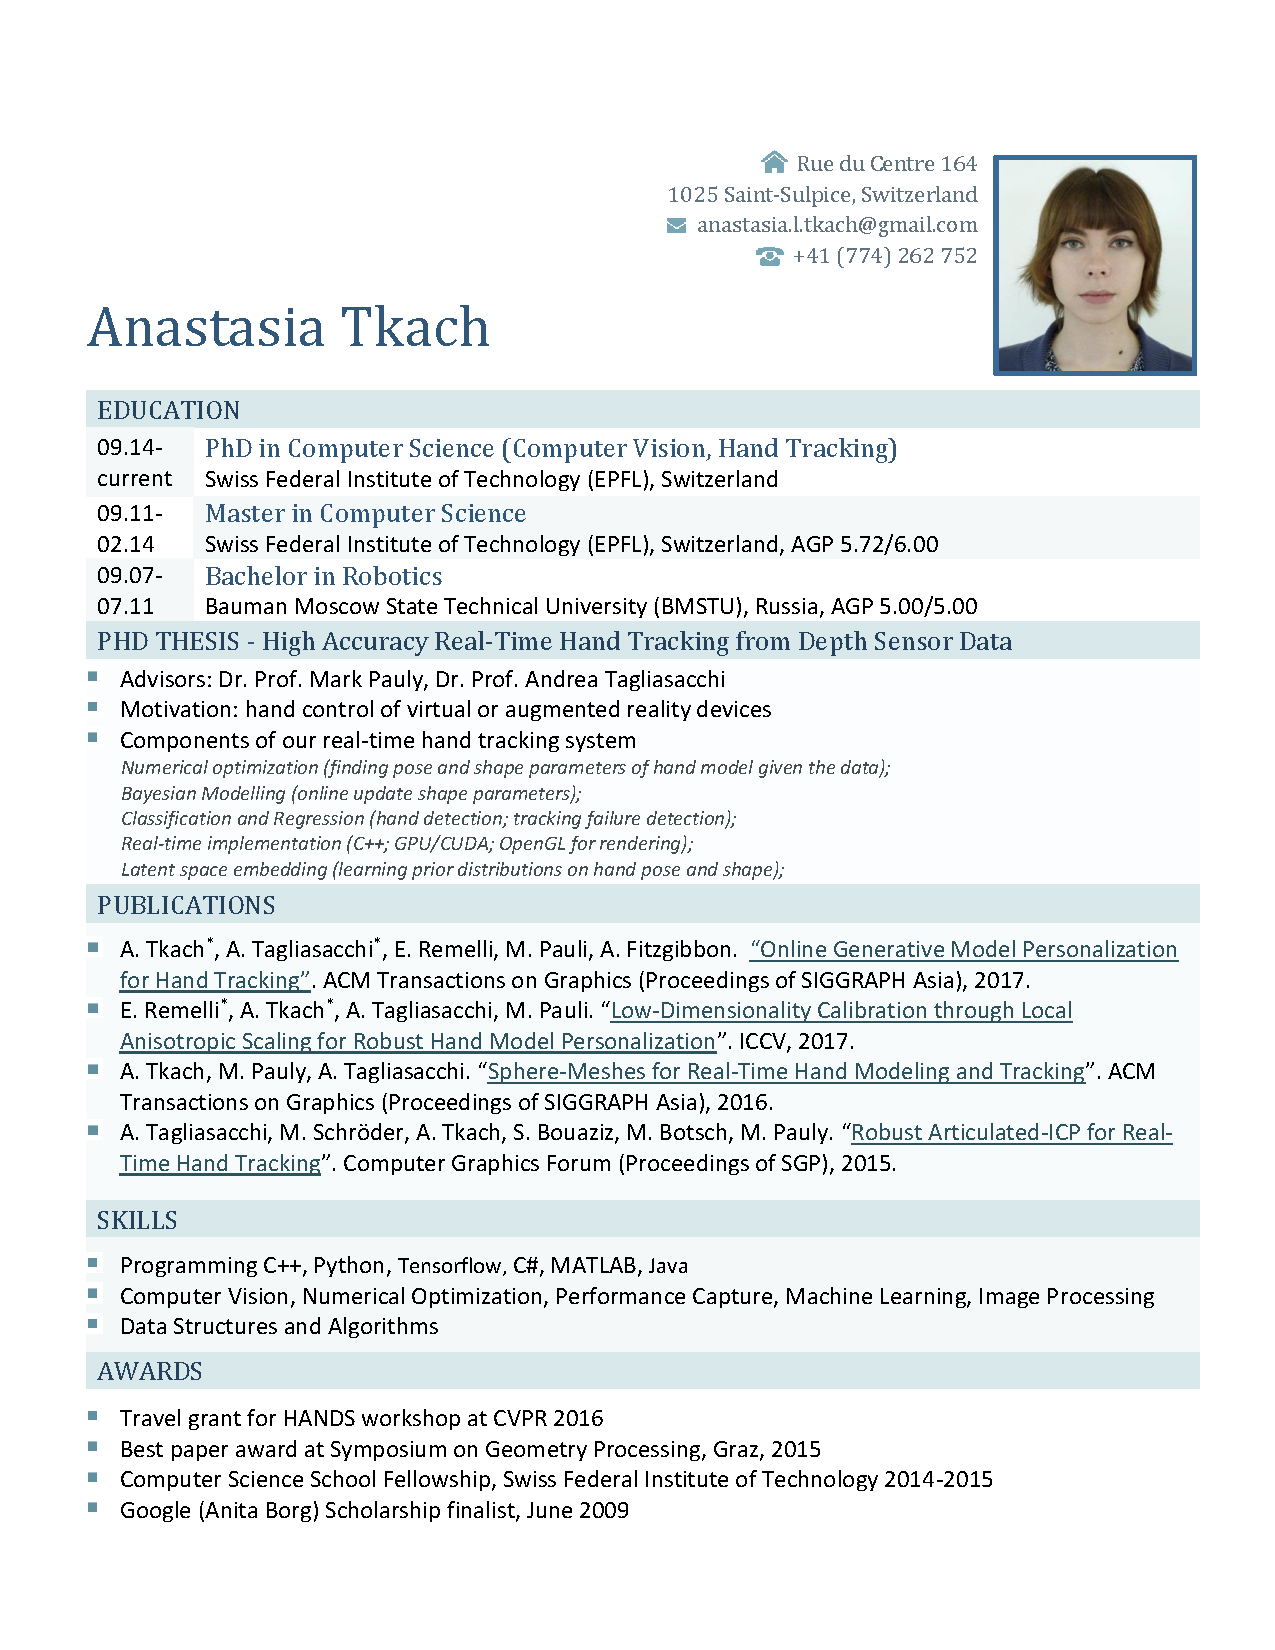
\includepdf[pagecommand=\thispagestyle{addpagenumbersforpdfimports},pages=-]{tail/cv.pdf}

\end{document}
